% ============================================================================
%  main.tex --- "Energy-Value Supervision for De Novo Molecular Flows:
%                Local Density Ordering Without Partition Functions"
%
%  Structure (after the 2026-08-19 compression pass):
%    Sec. 1  Introduction                       sections/01_intro.tex
%    Sec. 2  Energy-value supervision (2.1-2.4)  sections/02_method.tex
%    Sec. 3  From local ordering to connected supervision  sections/03_theory.tex
%    Sec. 4  Experiments (setting, protocol, results)  sections/04_experiments.tex
%    Sec. 5  Conclusion (limitations folded in) sections/05_conclusion.tex
%    App. A  Theory: assumptions, estimator, proofs   sections/A1_proofs.tex
%    App. B  Implementation and experimental details sections/A2_details.tex
%    App. C  Extended setting and related work        sections/A3_related.tex
%
%  Floats in the main text: exactly four figures, no table.
%    Figure 1  figures/fig1_objective_float.tex   (TikZ, Sec. 1)
%    Figure 2  figures/fig3_grid.tex              (matched grid, Sec. 4.1)
%    Figure 3  figures/fig2_ordering.tex          (ordering/retrieval, Sec. 4.2)
%    Figure 4  figures/fig4_calibration.tex       (calibration, Sec. 4.3)
%  The old Table 1 (tab:primary) now lives in App. B.7, caption intact.
%  No \resizebox anywhere.  Do not add a float without removing one.
%
%  Page budget: \label{endofmaintext} must land on page 9 or earlier.
%  Check with:  bash build.sh   (it prints MAIN TEXT PAGES from main.aux).
% ============================================================================

\documentclass{article} % ICLR uses plain article + the conference .sty

% --- REQUIRED: the conference style + Times. Do NOT add options.
%     iclr2027_conference.{sty,bst,bib}, math_commands.tex, natbib.sty and
%     fancyhdr.sty are the OFFICIAL ICLR 2027 author kit, taken unmodified from
%     media.iclr.cc/Conferences/ICLR2027/iclr-2027-style-files.zip on 2026-08-30.
%     Do not edit them.
\usepackage{iclr2027_conference,times}
% NOTE: the .sty already does \RequirePackage{natbib} and \setcitestyle{...}.
% Never write \usepackage[...]{natbib} yourself -> "Option clash for natbib".

% --- Math. amsmath must be loaded before math_commands.tex is \input.
\usepackage{amsmath,amssymb,amsthm}
\let\amseqref\eqref            % save amsmath's \eqref -> "(3)"
\input{math_commands.tex}      % \va \mA \E \R \Ls \Var \KL ...
\let\eqref\amseqref            % math_commands clobbers \eqref; undo.

\usepackage{graphicx}
\usepackage{booktabs}
\usepackage{array}
\usepackage{xcolor}
\usepackage{subcaption}        % unused directly, but it pulls in caption,
                               % which sets caption typography document-wide.
\usepackage{microtype}
\usepackage{tikz}              % required by figures/fig1_objective.tex

% --- Float typography.  Margins, body font and leading are untouched; only the
%     caption size and the space around floats are set, which is normal
%     practice and is what makes five floats fit inside the page budget.
\captionsetup{font=footnotesize,skip=3pt}
\setlength{\textfloatsep}{6pt plus 2pt minus 2pt}
\setlength{\floatsep}{5pt plus 2pt minus 2pt}
\setlength{\intextsep}{5pt plus 2pt minus 2pt}
\setlength{\abovedisplayskip}{5pt plus 2pt minus 2pt}
\setlength{\belowdisplayskip}{5pt plus 2pt minus 2pt}
\setlength{\abovedisplayshortskip}{3pt plus 2pt}
\setlength{\belowdisplayshortskip}{4pt plus 2pt}

% --- hyperref late; colorlinks is what real ICLR papers use.
\usepackage[colorlinks=true,linkcolor=blue!55!black,citecolor=green!45!black,
            urlcolor=blue!70!black]{hyperref}
\usepackage{url}
\usepackage{cleveref}          % must come after hyperref.

% --- Theorem environments (independent counters, running in document order).
%       MAIN TEXT (sections/03_theory.tex): prop:ident only.
%       APPENDIX A (statement and proof in sections/A1_proofs.tex):
%         lem:score, thm:certificate, cor:gauge, def:overlap, thm:l2g,
%         cor:basins, cor:empirical, prop:trap, prop:conflict,
%         prop:surrogate
%       (the force-gauge aside lem:forcegauge / thm:gauge was deleted in the
%        2026-08-29 appendix-compression pass; do not re-add it.)
%     Cite these through \Cref{<label>}, never by number.
\theoremstyle{plain}
\newtheorem{theorem}{Theorem}
\newtheorem{lemma}{Lemma}
\newtheorem{proposition}{Proposition}
\newtheorem{corollary}{Corollary}
\theoremstyle{definition}
\newtheorem{assumption}{Assumption}
\newtheorem{definition}{Definition}
\theoremstyle{remark}
\newtheorem{remark}{Remark}

% --- Title.  Alternatives recorded in REVISION_LOG.md; switching is a
%     single edit here and requires no change to the body text.
\title{Energy-Value Regularisation in Molecular Flows:\\
       Local Ordering and Estimator Sensitivity}

% ANONYMITY: leave \author untouched for submission.  With \iclrfinalcopy
% commented out the .sty prints "Anonymous authors / Paper under double-blind
% review" and ignores \author.  No names, institutions, repository URLs,
% cluster names or funders anywhere in the body or in a title footnote.
\author{Anonymous}

%\iclrfinalcopy   % UNCOMMENT ONLY for the camera-ready version.

\begin{document}
\maketitle   % also installs the "Under review ... at ICLR 2027" running head.

% --- Abstract, Sec. 1 Introduction, Figure 1.
% ============================================================================
%  01_intro.tex --- Abstract, Sec. 1 Introduction (+ Figure 1).
%
%  2026-08-30 REFRAME.  This is a POSITIVE METHOD paper: energy-value
%  supervision is an effective way to inject local physical ordering into a
%  bond-free de novo molecular flow.  Calibration and cross-basin mass are
%  SEPARATE targets, characterised precisely, never the dominant message.
%
%  Paragraph order: (P1) the application and the missing capability;
%  (P2) the method as a minimal, off-policy intervention; (P3) the evidence,
%  in the order held-out ordering -> retrieval -> matched controls ->
%  fixed-RMSD -> scope; (P4) three POSITIVE contribution bullets.
%
%  STATISTICAL REPORTING POLICY.  No t value, no p value, no "significant" /
%  "n.s." anywhere in the main text or in any figure.  Descriptive standard
%  only: arm mean +/- SEM over independent seeds, every seed point drawn,
%  absolute effect size, seed counts, launched/completed/diverged.
%
%  NO RESOLUTION SWEEP ANYWHERE.  The step-count sensitivity analysis was
%  deleted from the whole document, main text and appendix.  Do not add a
%  step count to the narrative here or anywhere else.
%
%  ATTRIBUTION.  The cession (the log-variance divergence, its cancellation of
%  Z(c) and off-policy estimation of it are prior work) is made ONCE, in the
%  related-work subsection Sec. 2.1.  Do not restate it here; bullet 1 points
%  at Sec. 2 instead.
% ============================================================================

\begin{abstract}
De novo 3D molecular generation methods learn distributions over composition and geometry, while
energy-targeted samplers assume a fixed system or a supplied molecular graph. We introduce
\emph{energy-value supervision} for the tractable positional density of a bond-free de novo flow:
flow matching plus one group-wise objective, penalising the variance of
$\log q_\theta(x \mid c) + E(c,x)/kT$ over local perturbations of a parent geometry, where
$q_\theta$ is read out by reversing the positional ODE with the discrete labels clamped. The
partition function cancels within each group, and the same divergence can be estimated off-policy
under an arbitrary reference measure, so the energy labels come from a transferable universal
potential and are pre-computed once, with no bond labels and no model rollouts. On a conservative held-out evaluation of $93$ disjoint parents scored by an
independent GFN2-xTB potential, the method raises the mean within-parent density--energy correlation
from $0.200$ to $0.369$, top-1 retrieval of the lowest-energy geometry from $20.2\%$ to $29.6\%$ and
top-3 from $49.5\%$ to $62.4\%$. Across completed runs, a matched six-cell study shows the gain
requires the correct geometry--energy correspondence: zero-energy and scrambled-energy controls do
not improve over flow matching. The gain persists on fixed-RMSD shells, ruling out
radial-distance variation as the sole explanation. An identifiability analysis characterises the objective's scope and identifies
connected supervision as the missing ingredient for controlling relative basin mass, and raw
calibration does not improve, indicating that ranking, calibration and global allocation ask for
distinct interventions.
\end{abstract}

\section{Introduction}
\label{sec:intro}

% --- P1: the application and the missing capability.
De novo 3D molecular generators create composition and geometry at once
\citep{edm,geoldm,semlaflow,symphony,flowmol3,zatom1}: they propose which atoms a molecule contains
and where those atoms sit, which a conformer generator handed a graph does not do. What they lack is
a way to make the geometries they prefer the geometries a physical potential prefers, and that
ingredient now exists. Universal machine-learned potentials return an energy $E(c,x)$ of near-DFT
quality for arbitrary compositions at negligible cost \citep{omol25,esen}, transferring across
chemical space rather than being fitted per system. Energy-targeted samplers already train tractable
densities against $e^{-E/kT}$ \citep{noe2019boltzmann,tbg,sbg,arbg,adjointsampling,idem,ewfm}, but
they assume a fixed system, or a supplied composition or graph, so their machinery does not reach a
generator that is still choosing what molecule to make. The opportunity is to use energy
\emph{values} to shape the density a de novo flow already defines; \Cref{sec:related} places both
literatures against that question, and \Cref{app:related} extends the discussion.

% --- P2: the method as a minimal, off-policy intervention.
We do this with a single additional term. A continuous normalising flow assigns a tractable
log-density to any geometry by reversing its own positional ODE and accumulating the divergence
\citep{ffjord}; we call this the \emph{clamped positional density} $\log q_\theta(x \mid c)$, the
discrete channels being held at their endpoint labels while the positions evolve. Over $K$ displaced
geometries of one parent, all sharing a composition $c$, we penalise
$\Var_k[\log q_\theta(x_k \mid c) + E(c,x_k)/kT]$, which is zero exactly when the density is
proportional to $e^{-E/kT}$ on that group (\Cref{sec:method}, \Cref{fig:objective}). Centring inside
a group deletes the unknown normaliser $Z(c)$. Separately, the same divergence can be estimated
under an arbitrary reference measure, and that is what makes the supervision \emph{off-policy}:
the objective is an expectation under whatever measure produced the displaced geometries, not under
the model, so every energy label is computed once, ahead of training, and read from disk like data:
one extra loss, pre-computed labels, no bond supervision, no rollouts, no reference sampler.

% --- P3: the evidence.
The intervention works, and we show what in it works. On $93$ held-out parents that the supervision
pool never contained, with every geometry re-scored by a GFN2-xTB potential that enters no training
loss, the mean per-parent correlation between $\log q_\theta$ and $-E/kT$ rises from
$0.200 \pm 0.018$ over five flow-matching seeds to $0.369 \pm 0.023$ over four completed value
seeds, a gain of $+0.169$ in which all four value seeds exceed all five control seeds. It converts
into a decision: ranking a parent's displaced geometries by $\log q_\theta$ retrieves the
lowest-energy one $29.6\%$ of the time against $20.2\%$, with $12.5\%$ at chance. A matched six-cell
grid then localises the effect, since zeroed energies and energies scrambled within a parent leave
ordering where flow matching leaves it, so what helps is the correct geometry-to-energy
correspondence and not the presence of an auxiliary penalty; a control holding displacement
magnitude fixed keeps the gain, ruling out radial-distance variation as the sole explanation. Finally an
identifiability analysis says how far the term reaches: it fixes the density--energy relation inside
a group up to one additive constant per connected component of the group-overlap graph, making group
connectivity a design variable and relative basin mass something a further objective must supply
(\Cref{sec:theory}).

% =====================================================================
%  fig1_objective_float.tex --- the float wrapper for Figure 1.
%
%  Figure 1 is pure TikZ, so this wrapper \input's the picture directly
%  rather than \includegraphics-ing a PDF (the same mechanism the old
%  fig1_method.tex used).  main.tex already loads tikz and amsmath.
%
%  Include from sections/01_intro.tex with:
%      % =====================================================================
%  fig1_objective_float.tex --- the float wrapper for Figure 1.
%
%  Figure 1 is pure TikZ, so this wrapper \input's the picture directly
%  rather than \includegraphics-ing a PDF (the same mechanism the old
%  fig1_method.tex used).  main.tex already loads tikz and amsmath.
%
%  Include from sections/01_intro.tex with:
%      \input{figures/fig1_objective_float}
%
%  The picture is drawn at 13.90cm = 5.47in, i.e. full ICLR single-column
%  width at scale 1.0.  Do NOT wrap it in \resizebox and do NOT scale it:
%  the in-figure type is \small / \footnotesize / \scriptsize of the 10pt
%  body font and scaling would desynchronise it from the caption.
%
%  PROVENANCE.  Conceptual figure, no data.  Built per the Figure 1 brief:
%  four panels (generator / teacher values / the value term / scope), and
%  the gradient-supervision branch of the superseded fig1_method.tex is
%  removed entirely rather than demoted.  No panel asserts a result.
%
%  REVISION C13 (figure-editor pass).  The framing moves to the method: panel
%  (c) is titled "Proposed energy-value supervision" and states inside the box
%  that the partition function cancels; panel (d)'s heading is "Local
%  supervision and the path to global control" and its closing line names the
%  extension (connecting groups so they share one offset) alongside the
%  unchanged qualification that b_B - b_A and the relative mass are not
%  identified.  No mathematical content was removed.
%
%  REVISION C8.  The caption is rewritten only where panels (c) and (d)
%  changed.  (c) now names the complete objective, so the caption states
%  it.  (d) now shows two disconnected groups of ONE composition, so the
%  caption no longer says the offset is free "between compositions"; the
%  freedom is already there inside a single conditional density.  The
%  verb "pins" is gone: the term CONSTRAINS THE LOCAL RELATION between
%  log-density and energy within a group.  The disconnection claim is
%  empirical and audited -- distinct parents sharing a composition supply
%  distinct perturbation clouds that share no sampled geometry (31% of
%  training parents sit on a repeated composition and are still
%  disconnected), so the overlap graph is a set of isolated vertices.
% =====================================================================
\begin{figure}[t]
  \centering
  \providecommand{\figOneScale}{1.0}\renewcommand{\figOneScale}{1.000}%
% SCALE = 1.000, THE FIGURE's NATURAL SIZE.  Do not lower it to buy page space.
% TikZ's `scale' multiplies COORDINATES but not type: every label in this
% picture is set at an absolute size (\small / \footnotesize / \scriptsize of
% the 10pt body), so any scale < 1 shrinks the panel frames out from under
% text that keeps its size, and the text runs out of the panels.
% MEASURED 2026-08-30 (600 dpi render of the standalone picture; panel frames
% located from the rendered strokes, so the calibration is self-checking at
% 236.22 px/cm on both axes):
%     scale 0.86 -> 4085 ink pixels outside the four panel frames, in 6
%                   regions.  Panel (b)'s body line runs to x = 14.59 cm,
%                   i.e. 0.71 cm past its own frame and 0.69 cm past the
%                   picture's 13.90 cm bounding box; panel (a)'s last two lines
%                   cross into panel (b)'s frame; panel (c)'s closing identity
%                   line crosses the left frame at x = -0.17 cm.
%     scale 1.000 -> 0 ink pixels outside the panels, at every ink threshold
%                   tested (lum < 128 and lum < 200, with 5 px of stroke
%                   tolerance).  All four panels are clean.
% PAGE COST: none that changes the budget.  With 1.000 the main text ends on
% page 9 and a probe \vspace inserted before \label{endofmaintext} shows a
% further +108pt fits before it spills to page 10 (+114pt spills); at 0.86 the
% same probe breaks between +108pt and +120pt.  The fix costs at most about
% one body line of final-page headroom.
  \input{figures/fig1_objective}
  \caption{\textbf{Energy-value supervision without a partition function.}
    Ideal-objective schematic; no measured quantity appears here. The archived implementation does not realise this density construction (\Cref{sec:method:impl}).
    \textbf{(a)}~With the endpoint discrete labels clamped, reversing the
    positional ODE defines the \emph{clamped positional-flow density}
    $\log q_\theta(x \mid c)$, which need not equal the joint generator's
    conditional density. \textbf{(b)}~A universal neural potential values each
    of $K$ displaced geometries of one parent. \textbf{(c)}~The proposed
    objective is flow matching plus the within-group variance of
    $\log q_\theta(x_k \mid c) + E_k/kT$, which vanishes exactly when
    $\log q_\theta = -E_k/kT + b$ inside the group: the partition function
    cancels and the offset $b$ is free. \textbf{(d)}~Two disconnected groups of
    the \emph{same} density keep independent offsets, so the term constrains
    the local density--energy relation inside each group and leaves their
    relative mass unidentified; connecting groups so they share one offset is
    the extension toward global control. Panel detail in \Cref{app:figdetail}.}
  \label{fig:objective}
\end{figure}

%
%  The picture is drawn at 13.90cm = 5.47in, i.e. full ICLR single-column
%  width at scale 1.0.  Do NOT wrap it in \resizebox and do NOT scale it:
%  the in-figure type is \small / \footnotesize / \scriptsize of the 10pt
%  body font and scaling would desynchronise it from the caption.
%
%  PROVENANCE.  Conceptual figure, no data.  Built per the Figure 1 brief:
%  four panels (generator / teacher values / the value term / scope), and
%  the gradient-supervision branch of the superseded fig1_method.tex is
%  removed entirely rather than demoted.  No panel asserts a result.
%
%  REVISION C13 (figure-editor pass).  The framing moves to the method: panel
%  (c) is titled "Proposed energy-value supervision" and states inside the box
%  that the partition function cancels; panel (d)'s heading is "Local
%  supervision and the path to global control" and its closing line names the
%  extension (connecting groups so they share one offset) alongside the
%  unchanged qualification that b_B - b_A and the relative mass are not
%  identified.  No mathematical content was removed.
%
%  REVISION C8.  The caption is rewritten only where panels (c) and (d)
%  changed.  (c) now names the complete objective, so the caption states
%  it.  (d) now shows two disconnected groups of ONE composition, so the
%  caption no longer says the offset is free "between compositions"; the
%  freedom is already there inside a single conditional density.  The
%  verb "pins" is gone: the term CONSTRAINS THE LOCAL RELATION between
%  log-density and energy within a group.  The disconnection claim is
%  empirical and audited -- distinct parents sharing a composition supply
%  distinct perturbation clouds that share no sampled geometry (31% of
%  training parents sit on a repeated composition and are still
%  disconnected), so the overlap graph is a set of isolated vertices.
% =====================================================================
\begin{figure}[t]
  \centering
  \providecommand{\figOneScale}{1.0}\renewcommand{\figOneScale}{1.000}%
% SCALE = 1.000, THE FIGURE's NATURAL SIZE.  Do not lower it to buy page space.
% TikZ's `scale' multiplies COORDINATES but not type: every label in this
% picture is set at an absolute size (\small / \footnotesize / \scriptsize of
% the 10pt body), so any scale < 1 shrinks the panel frames out from under
% text that keeps its size, and the text runs out of the panels.
% MEASURED 2026-08-30 (600 dpi render of the standalone picture; panel frames
% located from the rendered strokes, so the calibration is self-checking at
% 236.22 px/cm on both axes):
%     scale 0.86 -> 4085 ink pixels outside the four panel frames, in 6
%                   regions.  Panel (b)'s body line runs to x = 14.59 cm,
%                   i.e. 0.71 cm past its own frame and 0.69 cm past the
%                   picture's 13.90 cm bounding box; panel (a)'s last two lines
%                   cross into panel (b)'s frame; panel (c)'s closing identity
%                   line crosses the left frame at x = -0.17 cm.
%     scale 1.000 -> 0 ink pixels outside the panels, at every ink threshold
%                   tested (lum < 128 and lum < 200, with 5 px of stroke
%                   tolerance).  All four panels are clean.
% PAGE COST: none that changes the budget.  With 1.000 the main text ends on
% page 9 and a probe \vspace inserted before \label{endofmaintext} shows a
% further +108pt fits before it spills to page 10 (+114pt spills); at 0.86 the
% same probe breaks between +108pt and +120pt.  The fix costs at most about
% one body line of final-page headroom.
  % =====================================================================
%  fig1_objective.tex --- Figure 1: the objective and its scope
%
%  CONCEPTUAL FIGURE.  NO DATA.  No number in this figure is measured;
%  every glyph is a schematic.  Nothing here asserts a result.
%
%  Replaces the old five-band figures/fig1_method.tex, which was too
%  dense for a first-page explanatory figure and whose bands (b)/(c)
%  gave the gradient-supervision path equal visual status.  Per the
%  build brief the force branch is REMOVED from this figure entirely;
%  gradient supervision appears only later, as an experimental
%  comparator, and is not drawn here.
%
%  Pure TikZ.  No external images, no pgfplots, no \includegraphics,
%  no arrows.meta, no pgfmathrandom (byte-reproducible across compiles).
%  Okabe--Ito colour-blind-safe palette, semantics shared with
%  make_experiment_figures.py::PALETTE:
%     blue    model / flow / learned quantities
%     green   the value term (energy values, L_value)
%     orange  the teacher (universal neural potential)
%     grey    neutral structure
%  Vermilion (= gradient supervision) and purple (= scrambled control)
%  are deliberately ABSENT: neither concept appears in this figure.
%
%  USAGE
%   (a) standalone (verification / slides):   pdflatex fig1_objective.tex
%   (b) inside the paper -- main.tex already \usepackage{tikz} and
%       \usepackage{amsmath}:
%         \input{figures/fig1_objective_float}
%       or, if the writer prefers to own the float:
%         \begin{figure}[t]\centering
%           \input{figures/fig1_objective}
%           \caption{...}\label{fig:objective}
%         \end{figure}
%
%  SIZE.  Natural size 13.90cm x 8.80cm == 5.47in x 3.46in.
%  ICLR is a SINGLE 5.5in text column, so this is a full-text-width
%  figure at scale 1.0.  DO NOT rescale it and DO NOT wrap it in
%  \resizebox: every glyph inside is \small / \footnotesize /
%  \scriptsize of the 10pt body font, and scaling desynchronises
%  in-figure text from the caption.
%
%  LAYOUT.  A 2x2 grid, read left-to-right, top-to-bottom:
%    (a) the generator      composition AND geometry from one flow
%    (b) the teacher        energy values for K displacements of one parent
%    (c) the objective      L_ours = L_FM + lambda_E L_value, and nothing else
%    (d) the scope          two basins of ONE composition; offset free
%  Panel widths 6.80 / 6.78 cm; no wire crosses a panel boundary, so
%  there is no routing to collide with text.
%
%  REVISION C8 (this pass).  Two changes, both confined to panels (c)/(d):
%   * (c) now displays the complete objective, L_ours = L_FM + lambda_E
%     L_value, so the reader cannot infer a hidden force or anchor branch.
%     Neither branch was ever drawn here and neither is added.
%   * (d) previously drew two groups of two DIFFERENT compositions
%     (c_A, c_B).  That was wrong twice over.  It misstated the failure
%     mode -- the unidentified offset is already present WITHIN a single
%     conditional density -- and it flirted with the claim that one
%     composition contributes exactly one group, which the composition
%     audit refutes: in the training perturbation shard
%     (processed_data/omol25_4m_processed/perturbation_train_n30000_s0.pt)
%     30,000 parent groups carry only
%     22,822 distinct (element multiset, total charge) keys, 2,204 keys
%     are shared by more than one parent (9,382 parents, 31%; max
%     multiplicity 80).  Panel (d) therefore now shows two groups A and B
%     of the SAME composition c: two disconnected supervised regions of
%     one density p_theta(.|c), each with its own free offset b_A, b_B.
%     "ordering fixed" / "pinned" wording is replaced throughout by
%     "the local relation between log-density and energy is constrained".
%  In the EVALUATION population (val_data_processed.pt; the 120 grid
%  parents and the 93 primary parents) every parent has a distinct
%  composition, multiplicity 1 -- that is an audited property of the
%  evaluation set, not of the supervision design, and this figure does
%  not assert it.
% =====================================================================

% ---- standalone bootstrap (skipped when \input into a tikz-enabled doc) ----
\ifx\tikzpicture\undefined
  \documentclass[10pt]{article}
  % 0.05cm of slack past the 13.90cm bounding box so that the panel border
  % stroke width does not report a spurious overfull \hbox in standalone mode.
  \usepackage[paperwidth=14.40cm,paperheight=9.20cm,margin=0.20cm,noheadfoot]{geometry}
  \usepackage{amsmath,amssymb,bm}
  \usepackage{times}
  \usepackage{tikz}
  \setlength{\topskip}{0pt}
  \setlength{\parindent}{0pt}
  \pagestyle{empty}
  \begin{document}%
  \def\figOneFinish{\end{document}}
\fi
\providecommand{\figOneFinish}{\relax}
\providecommand{\figOneScale}{1.0}

\usetikzlibrary{positioning,calc,fit,backgrounds,arrows,shapes.geometric}

% ---------------------------------------------------------------- palette
% Okabe & Ito (2008), CVD-safe qualitative set.
\providecommand{\oiOrangeDefined}{}
\definecolor{oiOrange}{HTML}{E69F00}
\definecolor{oiSky}   {HTML}{56B4E9}
\definecolor{oiGreen} {HTML}{009E73}
\definecolor{oiBlue}  {HTML}{0072B2}
\definecolor{oiPurple}{HTML}{CC79A7}
\definecolor{oiGrey}  {HTML}{7F7F7F}
\definecolor{oiGreyL} {HTML}{C4C4C4}
\definecolor{oiGreyD} {HTML}{4D4D4D}

% ---------------------------------------------------------------- type
% Body 10pt Times => \small 9pt, \footnotesize 8pt, \scriptsize 7pt.
% Titles are 9pt bold; all explanatory text is 8pt; 7pt is used only for
% short qualifiers.  Nothing in this figure is smaller than 7pt.
\tikzset{
  fpanel/.style   ={rounded corners=2.4pt, draw=#1!55!white, line width=0.7pt,
                    fill=#1!4},
  ftitle/.style   ={anchor=north west, font=\small\bfseries, inner sep=0pt,
                    text=oiGreyD},
  fsub/.style     ={anchor=north west, font=\footnotesize, inner sep=0pt,
                    text=oiGrey, align=left},
  fbody/.style    ={anchor=north west, font=\footnotesize, inner sep=0pt,
                    align=left},
  fnote/.style    ={anchor=north west, font=\scriptsize, inner sep=0pt,
                    align=left, text=oiGreyD},
  fctr/.style     ={anchor=north, font=\footnotesize, inner sep=0pt,
                    align=center},
  fctrn/.style    ={anchor=north, font=\scriptsize, inner sep=0pt,
                    align=center, text=oiGreyD},
  flow/.style     ={-stealth', line width=1.0pt, draw=oiBlue},
  teach/.style    ={-stealth', line width=1.0pt, draw=oiOrange!88!black},
  freearr/.style  ={stealth'-stealth', line width=0.8pt, draw=oiGrey,
                    dash pattern=on 2.4pt off 1.8pt},
  eqbox/.style    ={rounded corners=2.4pt, draw=oiGreen!65!white,
                    line width=0.8pt, fill=oiGreen!8},
}

% ------------------------------------------------------- molecule glyphs
% Deterministic coordinates: the figure is identical on every compile.
\newcommand{\fAtom}[3]{\fill[#3] (#1,#2) circle (2.05pt);%
  \draw[oiGreyD!55, line width=0.2pt] (#1,#2) circle (2.05pt);}
\newcommand{\fAtomS}[3]{\fill[#3] (#1,#2) circle (1.35pt);%
  \draw[oiGreyD!45, line width=0.15pt] (#1,#2) circle (1.35pt);}
\newcommand{\fBond}[4]{\draw[oiGrey!80, line width=0.7pt] (#1,#2) -- (#3,#4);}

% t = 0 : unstructured cloud, no bonds, no identities
\newcommand{\fMolNoise}{%
  \fAtomS{-0.36}{ 0.32}{oiGreyL}\fAtomS{ 0.12}{ 0.38}{oiGreyL}%
  \fAtomS{ 0.38}{ 0.06}{oiGreyL}\fAtomS{-0.10}{-0.02}{oiGreyL}%
  \fAtomS{-0.42}{-0.28}{oiGreyL}\fAtomS{ 0.06}{-0.36}{oiGreyL}%
  \fAtomS{ 0.42}{-0.34}{oiGreyL}\fAtomS{ 0.26}{ 0.24}{oiGreyL}%
  \fAtomS{-0.18}{ 0.12}{oiGreyL}}

% t = 1 : a structure with distinguishable element identities.  Element
% colours are neutral (grey / blue / sky / purple) so they cannot be read
% as the semantic green (value) or orange (teacher).
\newcommand{\fMolFinal}{%
  \fBond{ 0.000}{ 0.30}{-0.285}{ 0.09}\fBond{-0.285}{ 0.09}{-0.176}{-0.25}%
  \fBond{-0.176}{-0.25}{ 0.176}{-0.25}\fBond{ 0.176}{-0.25}{ 0.285}{ 0.09}%
  \fBond{ 0.285}{ 0.09}{ 0.000}{ 0.30}%
  \fBond{ 0.285}{ 0.09}{ 0.600}{ 0.27}%
  \fBond{-0.285}{ 0.09}{-0.560}{ 0.32}%
  \fBond{-0.176}{-0.25}{-0.385}{-0.47}%
  \fAtom{ 0.000}{ 0.30}{oiGreyD!75}\fAtom{-0.285}{ 0.09}{oiGreyD!75}%
  \fAtom{-0.176}{-0.25}{oiGreyD!75}\fAtom{ 0.176}{-0.25}{oiGreyD!75}%
  \fAtom{ 0.285}{ 0.09}{oiBlue}%
  \fAtom{ 0.600}{ 0.27}{oiPurple}%
  \fAtomS{-0.560}{ 0.32}{oiSky}%
  \fAtomS{-0.385}{-0.47}{white}}

% the same structure, small, for the displacement cloud in panel (b)
\newcommand{\fMolSmall}[1]{%
  \draw[#1, line width=0.55pt]
    ( 0.000, 0.24) -- (-0.228, 0.07) -- (-0.141,-0.20) --
    ( 0.141,-0.20) -- ( 0.228, 0.07) -- cycle;
  \draw[#1, line width=0.55pt] ( 0.228, 0.07) -- ( 0.470, 0.22);
  \draw[#1, line width=0.55pt] (-0.228, 0.07) -- (-0.440, 0.25);
  \foreach \px/\py in {0/0.24, -0.228/0.07, -0.141/-0.20, 0.141/-0.20,
                       0.228/0.07, 0.470/0.22, -0.440/0.25}
    {\fill[#1] (\px,\py) circle (1.15pt);}}

% =====================================================================
\begin{tikzpicture}[x=1cm, y=1cm, scale=\figOneScale, >=stealth']
% stable bounding box
\path (0,0) rectangle (13.90,8.80);

% ---- panel frames ----------------------------------------------------
\draw[fpanel=oiBlue]   (0.02,4.85) rectangle (6.82,8.75);
\draw[fpanel=oiOrange] (7.10,4.85) rectangle (13.88,8.75);
\draw[fpanel=oiGreen]  (0.02,0.05) rectangle (6.82,4.55);
\draw[fpanel=oiGrey]   (7.10,0.05) rectangle (13.88,4.55);

% =====================================================================
% (a) THE GENERATOR
% =====================================================================
\node[ftitle] at (0.22,8.66) {(a) A de novo flow};
\node[fsub, text width=6.30cm] at (0.22,8.30)
     {composition \emph{and} geometry from one model};

% prior
\begin{scope}[shift={(1.15,7.34)}]\fMolNoise\end{scope}
\node[fctr, text width=2.60cm] at (1.32,6.66)
     {$x_0\sim\mathcal{N}(0,\sigma^{2}I)$};
\node[fctrn, text width=2.40cm] at (1.32,6.28) {random types};

% flow arrow
\draw[flow] (2.20,7.34) -- (3.90,7.34);
\node[anchor=south, font=\footnotesize, text=oiBlue!80!black] at (3.05,7.46)
     {$v_\theta(x_t,t)$};
\node[anchor=north, font=\scriptsize, text=oiGreyD] at (3.05,7.20)
     {flow matching};

% sample
\begin{scope}[shift={(5.15,7.34)}]\fMolFinal\end{scope}
\node[fctr, text width=2.60cm] at (5.15,6.66) {$(c,\,x)$};
\node[fctrn, text width=3.10cm] at (5.15,6.30)
     {atom types $c$, coordinates $x$};

\node[fbody, text width=6.46cm] at (0.22,5.94)
     {No bond labels anywhere. With the discrete labels
      clamped, reversing the positional ODE gives
      $\log q_\theta(x\mid c)$.};

% =====================================================================
% (b) THE TEACHER
% =====================================================================
\node[ftitle] at (7.30,8.66) {(b) Teacher energy values};
\node[fsub, text width=6.30cm] at (7.30,8.30)
     {$K$ displaced geometries of \emph{one} parent};

% displacement cloud: two faint copies + one dark reference structure
\draw[oiGrey!45, line width=0.5pt, dash pattern=on 1.8pt off 1.6pt]
      (8.35,7.24) circle (0.72);
\begin{scope}[shift={(8.19,7.40)}]\fMolSmall{oiGreyL}\end{scope}
\begin{scope}[shift={(8.54,7.10)}]\fMolSmall{oiGreyL}\end{scope}
\begin{scope}[shift={(8.33,7.22)}]\fMolSmall{oiGreyD!80}\end{scope}
\node[fctr, text width=2.40cm] at (8.35,6.36) {$x_1,\dots,x_K$};
\node[fctrn, text width=2.60cm] at (8.35,6.04) {same composition $c$};

% teacher arrow
\draw[teach] (9.28,7.24) -- (10.22,7.24);
\node[anchor=south, font=\footnotesize, text=oiOrange!55!black] at (9.75,7.36)
     {$E(c,\cdot)$};

% energy ladder
\draw[-stealth', line width=0.7pt, draw=oiGreyD] (10.72,6.42) -- (10.72,7.94);
\node[anchor=east, font=\footnotesize, text=oiGreyD] at (10.62,7.84) {$E$};
\foreach \yy in {6.58, 6.86, 7.12, 7.44, 7.74}
  {\draw[oiGrey!70, line width=0.5pt] (10.72,\yy) -- (11.06,\yy);
   \fill[oiOrange!85!black] (11.06,\yy) circle (1.6pt);}
\node[anchor=west, font=\footnotesize] at (11.24,7.62)
     {$E_k=E(c,x_k)$};
\node[anchor=north west, font=\scriptsize, text width=2.50cm, text=oiGreyD]
      at (11.24,7.30) {one value per geometry};

\node[fbody, text width=6.34cm] at (7.30,5.62)
     {A universal neural potential over $83$ elements supplies every
      value. Only the values are used.};

% =====================================================================
% (c) THE OBJECTIVE
% =====================================================================
\node[ftitle] at (0.22,4.46) {(c) Proposed energy-value supervision};

\draw[eqbox] (0.16,2.86) rectangle (6.68,4.06);
\node[anchor=center, font=\small] at (3.42,3.86)
     {$\mathcal{L}_{\mathrm{ours}}
       =\mathcal{L}_{\mathrm{FM}}+\lambda_E\,\mathcal{L}_{\mathrm{value}}$};
\node[anchor=center, font=\small] at (3.42,3.48)
     {$\mathcal{L}_{\mathrm{value}}
       =\mathrm{Var}_{k}\big[\,\log q_\theta(x_k\mid c)+E_k/kT\,\big]$};
% The cancellation is the selling point of the objective, so it is drawn in
% the value colour rather than in neutral grey.  It is a statement about the
% objective, not a measured claim.
\node[anchor=north, font=\scriptsize, inner sep=0pt, align=center,
      text=oiGreen!45!black, text width=6.20cm] at (3.42,3.22)
     {one added term; the partition function cancels};

% schematic alignment plot
\draw[oiGreyD, line width=0.7pt] (1.36,2.52) -- (1.36,1.02) -- (3.98,1.02);
\node[rotate=90, anchor=south, font=\footnotesize, text=oiGreyD]
      at (1.20,1.77) {$\log q_\theta$};
\node[anchor=north, font=\footnotesize, text=oiGreyD] at (2.70,0.94)
     {$-E_k/kT$};
% the line the value term asks for: slope one, offset free
\draw[oiGreen!70!black, line width=0.9pt, dash pattern=on 2.6pt off 1.8pt]
      (1.52,1.16) -- (3.82,2.40);
% unconstrained (grey) and aligned (green) geometries
\foreach \px/\py in {1.68/2.12, 2.02/1.24, 2.36/2.32, 2.72/1.42,
                     3.08/1.98, 3.46/1.30, 3.72/2.20}
   {\fill[oiGrey!75] (\px,\py) circle (1.7pt);}
\foreach \px/\py in {1.68/1.22, 2.02/1.42, 2.36/1.50, 2.72/1.76,
                     3.08/1.92, 3.46/2.14, 3.72/2.36}
   {\fill[oiGreen] (\px,\py) circle (1.7pt);}
% legend
\fill[oiGrey!75] (4.42,2.32) circle (1.7pt);
\node[anchor=west, font=\footnotesize, text width=2.00cm] at (4.58,2.32)
     {$\mathcal{L}_{\mathrm{value}}$ large};
\fill[oiGreen] (4.42,1.86) circle (1.7pt);
\node[anchor=west, font=\footnotesize, text width=2.00cm] at (4.58,1.86)
     {$\mathcal{L}_{\mathrm{value}}=0$};
\node[fnote, text width=2.30cm] at (4.30,1.50)
     {one variance per group};

\node[anchor=north, font=\scriptsize, text=oiGreyD] at (3.42,0.56)
     {$\mathcal{L}_{\mathrm{value}}=0$ within a group
      $\iff \log q_\theta=-E_k/kT+b$};

% =====================================================================
% (d) THE SCOPE
% =====================================================================
% Two lines of \small\bfseries; the composition fact that used to sit in a
% separate subtitle is folded into the region label below, which is where the
% single conditional density is named anyway.
\node[ftitle, text width=6.50cm, align=left] at (7.30,4.46)
     {(d) Local supervision and the\\path to global control};

% the enclosing region: ONE conditional density, several supervised groups
\draw[rounded corners=2.8pt, draw=oiGrey!50, line width=0.6pt,
      dash pattern=on 2.2pt off 1.8pt] (7.42,1.02) rectangle (13.56,3.54);
\node[anchor=center, font=\scriptsize, text=oiGreyD, inner sep=1.6pt,
      fill=oiGrey!4] at (10.49,3.54)
     {one density $q_\theta(\cdot\mid c)$ --- same composition $c$};

\foreach \cx/\lbl in {8.86/A, 12.12/B}
{%
  \node[anchor=north, font=\footnotesize] at (\cx,3.36)
       {group $\lbl$ (basin $\lbl$)};
  \draw[oiGreen!60!white, line width=0.8pt, fill=oiGreen!7]
        (\cx,2.38) ellipse (1.28 and 0.56);
  \draw[oiGreen!45!black, line width=0.6pt]
        (\cx-0.88,2.26) -- (\cx-0.44,2.52) -- (\cx,2.36)
        -- (\cx+0.44,2.69) -- (\cx+0.84,2.50);
  \foreach \dx/\yy in {-0.88/2.26, -0.44/2.52, 0.00/2.36,
                        0.44/2.69, 0.84/2.50}
    {\fill[oiGreen] (\cx+\dx,\yy) circle (1.7pt);}
  \node[anchor=north, font=\scriptsize, text=oiGreyD] at (\cx,1.74)
       {local relation constrained};
  \node[anchor=north, font=\footnotesize] at (\cx,1.46)
       {offset $b_{\lbl}$ free};
}

\draw[freearr] (10.16,2.38) -- (10.82,2.38);
\node[anchor=south, font=\footnotesize, text=oiGrey] at (10.49,2.46) {?};

% Same mathematical content as before -- b_B - b_A and the relative mass are
% not identified -- with the constructive half of the statement added: what
% would have to be built to identify them.  No claim is weakened.
% WIDTH BUDGET.  The float sets \figOneScale = 1.000 and the picture is measured
% at that scale (see the measurement note in fig1_objective_float.tex: at 1.000 a
% 600 dpi render has zero ink outside the four panel frames; at 0.86 it has 4085
% such pixels, because tikz's `scale' shrinks COORDINATES but not type).  Panel
% (d) is 6.78cm wide at scale 1.000 and every font size here is absolute.  Two lines of at most ~42 \footnotesize characters is the whole
% budget; anything longer runs out of the panel and into panel (c).  Both qualifications survive the compression: the offset
% DIFFERENCE and the relative mass are the two unidentified quantities, and the
% second line names the extension that would identify them.
\node[anchor=north, font=\footnotesize, align=center]
      at (10.49,0.92)
     {$b_B-b_A$, relative mass: not identified.\\
      Connecting groups would share one offset.};

\end{tikzpicture}

\figOneFinish

  \caption{\textbf{Energy-value supervision without a partition function.}
    Ideal-objective schematic; no measured quantity appears here. The archived implementation does not realise this density construction (\Cref{sec:method:impl}).
    \textbf{(a)}~With the endpoint discrete labels clamped, reversing the
    positional ODE defines the \emph{clamped positional-flow density}
    $\log q_\theta(x \mid c)$, which need not equal the joint generator's
    conditional density. \textbf{(b)}~A universal neural potential values each
    of $K$ displaced geometries of one parent. \textbf{(c)}~The proposed
    objective is flow matching plus the within-group variance of
    $\log q_\theta(x_k \mid c) + E_k/kT$, which vanishes exactly when
    $\log q_\theta = -E_k/kT + b$ inside the group: the partition function
    cancels and the offset $b$ is free. \textbf{(d)}~Two disconnected groups of
    the \emph{same} density keep independent offsets, so the term constrains
    the local density--energy relation inside each group and leaves their
    relative mass unidentified; connecting groups so they share one offset is
    the extension toward global control. Panel detail in \Cref{app:figdetail}.}
  \label{fig:objective}
\end{figure}


\begin{itemize}\itemsep0pt\parskip0pt\topsep2pt\leftmargin1.2em
\item \textbf{Method.} Energy-value supervision for de novo molecular flows: a group-wise variance
  objective, whose divergence form is standard and is credited in \Cref{sec:method}, applied to the
  clamped positional density of a bond-free generator over an 83-element corpus, with pre-computed
  values from a transferable potential, no bond labels, no rollouts and no partition function.

\item \textbf{Controlled evidence.} A matched six-cell study and a conservative held-out endpoint
  under an independent scorer, showing improved local ordering and retrieval and attributing both to
  the correct geometry--energy pairing rather than to regularisation, the energy multiset alone, or
  displacement magnitude.

\item \textbf{Characterisation and design guidance.} A result identifying what group-wise value
  supervision determines --- the local density--energy relation up to one offset per connected
  component of the overlap graph --- turning the objective's scope into a design criterion: local
  groups suffice for local ordering, and connected groups or a global term are what basin mass
  requires (\Cref{sec:theory}).
\end{itemize}


% --- Sec. 2 Energy-value supervision for de novo molecular flows.
% ============================================================================
%  02_method.tex --- Sec. 2, Energy-Value Supervision.  No floats.
%
%  2026-08-30 REFRAME.  Sec. 2 is the METHOD section of a method paper.
%  2026-08-30 RELATED-WORK PASS.  A compact related-work subsection was
%  PROMOTED from Appendix C (sections/A3_related.tex) and is now 2.1, so the
%  positioning is in the main text where a reviewer will find it.  Sec. 2 now
%  has five subsections:
%    2.1  related work: three groups + the intersection sentence   <-- promoted
%    2.2  the bond-free flow and its clamped positional density
%    2.3  the group-wise value objective          <-- BOXED, visually dominant
%    2.4  why the partition function cancels      <-- and why grouping is forced
%    2.5  a gradient-supervision baseline         <-- comparator, NOT a component
%
%  The proposed objective is the only boxed display in the paper.  The force
%  baseline in 2.5 must never be boxed or otherwise made to compete with it.
%
%  ATTRIBUTION IS MADE IN 2.1 AND NOWHERE ELSE.  The log-variance divergence,
%  the cancellation of Z(c) and off-policy estimation are prior work; 2.4
%  states the technical consequence and cross-references 2.1 for the credit.
%  Do NOT restore the citation list in 2.4 -- that would double-credit.
%
%  NOTATION.  lambda_E and L_value throughout; the historical code field is
%  named once, in 2.2.  kT_eff, never T_eff.  log q_theta, never log p_theta.
%
%  2026-08-19.  The eps = 1/(2n) SMOOTHED-MARGINAL READING IS WRONG AND HAS
%  BEEN DELETED (paper/ESTIMATOR_SEMANTICS.md).  Do not reinstate it.
% ============================================================================

\section{Energy-Value Supervision for De Novo Molecular Flows}
\label{sec:method}

\subsection{Related work: two literatures, and the question between them}
\label{sec:related}

\paragraph{De novo 3D molecular generation.} Equivariant diffusion and flow-matching models
generate positions and types jointly, from EDM and GeoLDM \citep{edm,geoldm} through
graph-and-geometry hybrids \citep{midi,symphony,semlaflow} to FlowMol3 \citep{flowmol3}, the
backbone used here, and Zatom-1 \citep{zatom1}, the one published generator trained on the same
corpus; EBMol \citep{ebmol} learns a scalar energy from data rather than from a physical potential.
These models are judged on validity, on sample quality, or on an energy the model itself learns, and
they define the state of the art at the task they set out to do. What such evaluations generally do
not ask is whether the tractable density the model defines responds to an \emph{external} physical
energy. That is a different question rather than a shortfall --- it is not the question these papers
pose --- and we claim superiority over none of them.

\paragraph{Conditional conformer and ensemble models.} Torsional diffusion \citep{torsionaldiff},
the GEOM conformer literature \citep{geom} and DECAF \citep{decaf} take the molecular graph, or the
molecular identity, as input and return conformers for it. The composition is supplied rather than
generated, so the density they define is conditional on a fixed chemical graph. That input is what
makes theirs a different problem from a de novo generator's, and why their protocols do not transfer
to one unchanged.

\paragraph{Energy-targeted samplers, and where our objective comes from.} Samplers that target
$e^{-E/kT}$ directly \citep{noe2019boltzmann,tbg,sbg,arbg,adjointsampling,idem,ewfm} obtain
equilibrium densities; mass-covering correction by annealed importance sampling \citep{fab}
addresses the cross-group failure that \Cref{cor:basins} formalises, potential-score matching
\citep{psm} supervises with the potential's gradient instead of its value, and \citet{idflow} drive
a predictor--refiner with an \emph{internal, learned} energy instead of an external one. Each takes
the system, the alphabet or the molecular graph as given: Adjoint Sampling \citep{adjointsampling},
the closest use of a universal potential as a training signal, trains against an eSEN energy but
samples conformers of a \emph{given} molecular graph. They therefore solve a stronger sampling
problem --- equilibrium, not ordering --- on a state space that is narrower and fixed in advance.
Our value term is inherited from this literature and is not claimed as new:
$\Var[\log q_\theta + E/kT]$ is the \emph{log-variance divergence} named by \citet{vargrad}, placed
in a path-space family by \citet{nusken2021pathspace}, given an optimal-control reading by
\citet{berner2024optimalcontrol} and established for diffusion samplers by
\citet{richter2024improvedsampling}; that a variance annihilates the normalising constant, and that
the divergence may be estimated off-policy under an arbitrary reference measure
\citep{sendera2024offpolicy}, are structural properties of that family, and we claim neither.

\paragraph{The intersection.} Existing de novo generators decide what molecule and what geometry to
produce, but do not test the tractable density they define against a transferable physical energy;
energy-targeted samplers test or optimise exactly that relation, but assume the molecular system or
the graph. This paper works at the intersection, asking what group-wise energy \emph{values} from a
universal potential do to the density of a generator that is still choosing its molecule. To our
knowledge the combination studied here --- an external universal potential supervising the
tractable density of a bond-free de novo flow --- has not been evaluated in this form.
\Cref{app:related} gives the formal setting and the fuller discussion.

\subsection{The bond-free flow and its clamped positional density}
\label{sec:method:flow}

A molecular state is a pair $(c,x)$: a composition $c$, the element multiset together with the total
charge, and a centre-of-mass-free conformation $x \in \R^{3N}$. The backbone is FlowMol3
\citep{flowmol3}, an SE(3)-equivariant conditional flow-matching model
\citep{lipman2023flowmatching,liu2023rectifiedflow,albergo2023interpolants} with
$x_t = (1-t)x_0 + t x_1$, $x_0 \sim \mathcal{N}(0,\sigma^2 I)$ at $\sigma = 1$, and
$\Ls_{\mathrm{FM}}$ the velocity-regression loss; types and charges ride a continuous-time Markov
chain. \emph{De novo} describes that backbone and its task; every energy measurement here is instead
conditional on a fixed endpoint composition, types and charges held at their data values whenever
the teacher is queried. The teacher is the universal neural potential trained on OMol25
\citep{omol25,esen}: 83 elements, DFT energies and forces, no bond labels, making the generator
bond-free by necessity, bonds recovered post hoc where an evaluation needs them \citep{xyz2mol}. It
supplies $E(c,x)$ in eV and $F = -\nabla_x E$, so
$\pi(x \mid c) = e^{-E(c,x)/kT}/Z(c)$; neither $Z(c)$ nor $\sum_c Z(c)$ is ever formed, and
$kT = 1.0$~eV is a \emph{numerical} target that keeps $E/kT$ tame, not a physical temperature.
Queries pass charge only and default to a singlet, so every evaluation below is on main-group
organic parents (\Cref{ass:charge}).

Because the generator is a continuous normalising flow, its log-density follows from the
instantaneous change of variables \citep{ffjord}: integrating the field backwards from $x_1$ and
accumulating the divergence gives
\begin{equation}
  \log q_\theta(x_1 \mid c) \;=\; \log p_0(x_0) - \int_0^1 \nabla \!\cdot\, v_\theta(x_t,t)\,\mathrm{d}t ,
  \label{eq:ffjord}
\end{equation}
with the trace estimated by Rademacher--Hutchinson probes \citep{hutchinson}. Throughout,
$q_\theta(x \mid c)$ is the \emph{clamped positional density}: \eqref{eq:ffjord} integrated with the
discrete channels, atom types, formal charges and the empty bond tensor, held at their endpoint
labels for the whole reverse trajectory, only the positions evolving. It costs one reverse solve per
geometry, is normalised on the centre-of-mass-free subspace by construction, and is the object this
paper supervises and evaluates. \textbf{It need not equal the joint generator's
conditional density $p_\theta(x \mid c)$}: the two coincide only if the discrete trajectory is
determined by its endpoint, and we have not quantified the difference (\Cref{ass:A2}).

\subsection{The group-wise value objective}
\label{sec:method:obj}

The intervention constrains the \emph{value} of that log-density rather than its gradient. The
Boltzmann residual $w(x) = \log q_\theta(x \mid c) + E(c,x)/kT$ is constant exactly where
$q_\theta(\cdot \mid c) \propto e^{-E(c,\cdot)/kT}$, so asking only that $w$ be \emph{flat} across a
set of geometries asks for the physics and nothing else. We pre-compute shards of $K$ perturbations
per parent, each carrying its teacher energy; every step draws $M$ parents and penalises the
variance of the residual inside each group:
\begin{equation}
  \boxed{\;
  \begin{aligned}
    \Ls_{\mathrm{ours}} \;&=\; \Ls_{\mathrm{FM}} \;+\; \lambda_E \,\Ls_{\mathrm{value}} ,
    \qquad
    \Ls_{\mathrm{value}} \;=\; \frac{1}{M}\sum_{m=1}^{M} \Var_k\bigl( w_{m,k} \bigr) ,
    \\[1pt]
    w_{m,k} \;&=\; \log q_\theta(x_{m,k} \mid c_m) \;+\; E_{m,k}/kT .
  \end{aligned}
  \;}
  \label{eq:lvalue}
\end{equation}
where $w_{m,k}$ is the residual at the $k$-th geometry of parent $m$, evaluated with that parent's
own composition $c_m$ and pre-computed teacher energy $E_{m,k}$. We use
$\lambda_E = 3\times10^{-5}$ (code field: \texttt{lambda\_2}), zero over a flow-matching warm-up and
then ramped, applied every few steps because each evaluation is a reverse-time solve carrying second
derivatives (\Cref{app:hyper}). Nothing else changes: same backbone, optimiser and data, no bond
labels, and the model we report as ours sets $\lambda_1 = 0$ and the anchor weight
$\lambda_3 = 0$.

\subsection{Why the partition function cancels, and why grouping is mandatory}
\label{sec:method:cancel}

Three properties of \eqref{eq:lvalue} do the work. First, $\log Z(c)$ enters $w$ as an additive
constant and a variance annihilates additive constants, so the normaliser cancels within a group and
is never formed --- the reason values from a transferable potential are usable at all, since $Z(c)$
changes with every composition. Second, grouping is mandatory rather than convenient, precisely
because that constant differs across molecules: its spread is set by size and composition rather
than by deviation from the Boltzmann law, so a variance over a batch of \emph{different} molecules
would measure the spread of $\log Z$ instead (\Cref{rem:crossbatch}).
Third, and separately from the cancellation, \eqref{eq:lvalue} is a group-wise estimate, against the
unnormalised Gibbs weight, of the \emph{log-variance divergence}, which may be estimated under an
\emph{arbitrary} reference measure. That, and not the cancellation, is what makes the supervision
off-policy and pre-computed shards valid: no sample need come from the model. The divergence, the
cancellation of $Z(c)$ inside it, and its off-policy estimation are prior work, credited in
\Cref{sec:related}. Ours is the deployment: a group-conditioned use of that estimator inside a mixed
discrete--continuous, bond-free de novo generator, at the price of one free constant per group
(\Cref{sec:theory}).

\paragraph{Practicalities.}
\label{sec:method:impl}
\emph{(i)} $\lambda_E$ was fixed once from a smoke run before any Boltzmann evaluation and never
tuned against a reported metric; the weight is small, its \emph{contribution} is not.
\emph{(ii)} \eqref{eq:ffjord} is integrated in $n$ explicit Euler steps over the whole of $[0,1]$,
the divergence integral by the midpoint rule on the same interval; the interval is not truncated, so
$n$ controls discretisation error rather than which density is meant (\Cref{app:estimator}).
Training uses $n = 4$ and every reported evaluation $n = 12$. \emph{(iii)} The reverse-time solve back-propagates second derivatives through a stochastic
trace, and runs carrying it reach non-finite weights at a rate that runs without it do not ($6$ of
$20$ against $0$ of $10$ in the matched grid of \Cref{sec:ablation}); a guard aborts on the first
non-finite parameter, and because divergence is not independent of the objective, \textbf{every
value-cell mean we report is conditional on completion}, with launched, completed and diverged
counts beside it. \emph{(iv)} The gradient through $\Ls_{\mathrm{value}}$ is a
\emph{truncated-adjoint surrogate}: the reverse trajectory is advanced without gradient tracking,
each state detached from the previous, so gradient flows only through the divergence evaluations; we
do not differentiate through the solve and do not claim exact likelihood training
(\Cref{app:asimplemented}).

\subsection{A gradient-supervision baseline}
\label{sec:forcebaseline}

The obvious alternative to values is the potential's gradient, measured separately under the same
backbone and budget. Flow matching gives the score of its time-$t$ marginal in closed form
(\Cref{lem:score}), $s_\theta(x_t,t) = [\,t\, v_\theta(x_t,t) - x_t\,]/[(1-t)\,\sigma^2]$, which at
the Boltzmann optimum equals $F/kT$, so a natural comparator regresses one on the other,
\begin{equation}
  \Ls_{\mathrm{force}}
  = \E_{t^{*},(c,x_1)}\Bigl[\, N(c)^{-1} \textstyle\sum_{i}
  \ell\bigl( s_\theta(x_{t^{*}}, t^{*})_i - \tfrac{F(c,x_1)_i}{kT} \bigr) \Bigr] .
  \label{eq:score}
\end{equation}%
The read-out has a pole at $t = 1$, so we probe only at $t^{*} \in \{0.85, 0.92, 0.97\}$ and average
a per-atom Huberised, norm-capped error $\ell$ (\Cref{app:constants}). The force target is read at
the data endpoint $x_1$ while the score is read on the conditional path, so this is a naive
off-policy endpoint form of force matching, a comparator and not a component of \eqref{eq:lvalue}: the model we report as ours has
$\lambda_1 = 0$, and results from $\lambda_1 > 0$ are labelled as such (\Cref{sec:ablation}).


% --- Sec. 3 From local ordering to connected supervision.
\section{From Local Ordering to Connected Supervision}
\label{sec:theory}

\eqref{eq:lvalue} sums \emph{within-group} variances, so the question worth asking is what a model
that drove it to zero would have been shown; the answer is precise enough to use as a design rule.
It concerns $q_\theta$ rather than $p_\theta(x \mid c)$, and the zero set of the ideal residual
condition rather than the implemented update's trajectory. Write
$w(x) = \log q_\theta(x \mid c) + E(c,x)/kT$, let $\rho_j$ be the reference measure of group $j$ with
support $U_j$, and join two groups by an edge of the \emph{overlap graph} $\mathcal{G}_c$ when
$\rho_j$ and $\rho_{j'}$ are not mutually singular, a property of the measures for which
$U_j \cap U_{j'} \neq \emptyset$ is necessary but far from sufficient (\Cref{def:overlap}).

\begin{proposition}[What zero group-wise variance fixes]
\label{prop:ident}
For strictly positive group weights $\pi_j$ and finite second moments, let the population objective $\sum_j \pi_j \Var_{\rho_j}[w]$ vanish. Then \emph{(i)} $w \equiv b_j$
$\rho_j$-almost surely on $U_j$ for a scalar $b_j$: the residual is fixed to one constant per group,
and no normaliser is needed, since $Z(c)$ enters $w$ only through that constant.
\emph{(ii)} $b_j = b_{j'}$ along every edge of $\mathcal{G}_c$, so the constants agree within each
connected component; connectivity is sufficient; in the unrestricted measurable residual class a disconnected graph permits different constants. Continuity or model-class restrictions can impose further relations. \emph{(iii)} If the $\rho_j$
have positive Lebesgue densities and $\mathcal{G}_c$ has $C \ge 2$ components $U^{(1)},\dots,U^{(C)}$
with finite positive restricted partition integrals and carrying all the model's mass, the zero-loss densities form a $(C-1)$-parameter family
$q_\theta = a_i e^{-E/kT}$ on $U^{(i)}$ with $\sum_i a_i Z^{(i)} = 1$, in which every vector of
component occupancies in the open simplex is attained: the \emph{relative} mass of separated
components is not identified.
\end{proposition}

\Cref{thm:l2g} states this in full, with the connected case and its two further hypotheses, and
\Cref{app:l2g} proves it. Our runs sit in the empirical reading (\Cref{cor:empirical}): $\rho_j$ is
the empirical measure on a group's $K$ sampled geometries, zero loss is $K-1$ scalar equations at
those points and nothing about unsampled ones, and parts (ii) and (iii) survive only as an
identifiability statement.

\paragraph{What our design supervises.} Each parent contributes exactly one group, and distinct
parents draw displacements independently from continuous distributions, so with probability one no
two groups share a sampled point: $\mathcal{G}_c$ is a set of isolated vertices and only part~(i)
applies (\Cref{cor:basins}). Part~(i) describes an ideal zero residual, which the experiments do not achieve --- the archived readout is not a validated $\log q_\theta$ --- and its complement is equally exact, the cloud's offset being free and the
relative probability of distinct basins untouched. Disconnection rests on mutual singularity rather
than on one group per composition, which our pool does not satisfy: $31\%$ of its parents sit on a
repeated composition, and those clouds are still disconnected (\Cref{app:l2g,app:data}). Nothing
above predicts the \emph{magnitude} of a correlation or the calibration of $\log q_\theta$
(\Cref{app:scope}), which are separate quantities measured separately in \Cref{sec:scale}.

\paragraph{The design criterion.} The analysis therefore turns an ambiguity into a design choice.
Connectivity is a property of the supervision graph, not of the model or the potential: local groups
suffice for local ordering, which is what we build and measure, while controlling relative basin
mass requires either a connected supervision graph --- groups tiled along a path between basins, so
part~(ii) propagates one constant across them --- or an additional global objective. This paper
measures local ordering; \Cref{app:nonequilibrium} specifies a global path-weight correction
as a separate development branch, without claiming established molecular benefit.


% --- Sec. 4 Experiments: setting, protocol, metrics, then the three result
%     subsections.  Figures 2-4.  (The former Sec. 4/Sec. 5 split was merged on
%     2026-08-30; do not re-split it.)
% ============================================================================
%  04_experiments.tex --- Sec. 4, the single Experiments section.
%
%  2026-08-30 MERGE PASS.  The former Sec. 4 "Experimental Design" and Sec. 5
%  "Results" are ONE section now: a setting-and-protocol block (shared setting,
%  the two tracks, metrics, reporting) runs straight into the three result
%  subsections, whose titles are unchanged.  Do not re-split them.  The labels
%  sec:setup / sec:protocol / sec:metrics / sec:experiments all now point at
%  this one section.  VERIFIED 2026-08-30: only sec:setup is actually cited
%  (A1_proofs.tex:704, 863); the other three are kept as spare anchors so an
%  appendix cross-reference written against any of the four still resolves.
%
%  Floats: Figure 2 (fig:grid, matched grid, Sec. 4.1), Figure 3 (fig:ordering,
%  ordering + retrieval + fixed-RMSD, Sec. 4.2), Figure 4 (fig:calibration).
%
%  2026-08-30 REFRAME + STATISTICAL REPORTING POLICY.
%    * ZERO t values, ZERO p values, ZERO "significant"/"n.s." in this file.
%      Descriptive standard only: arm mean +/- SEM over independently trained
%      seeds, absolute effect size Delta r, seed counts, and
%      launched/completed/diverged wherever completion differs by arm.
%      Applied in BOTH directions: the favourable statistics went too.
%    * There is NO resolution / step-count sensitivity analysis anywhere in
%      the paper: it was deleted from main text AND appendix.  Do not
%      re-introduce a step count into the narrative; the estimator is named
%      as an ODE integration of the clamped positional flow with Hutchinson
%      divergence estimation, and its settings live in the app:constants row.
%    * The adverse seed imputations are NOT printed here; app:eval carries
%      them and is the actual location of those numbers.
%
%  DESIGN IS ORGANISED BY EVIDENCE TRACK, NOT BY CHRONOLOGY.
%    Track A  matched mechanism grid, 120 parents, six cells.
%    Track B  the conservative held-out endpoint, 93 parents.
%
%  RELOCATED, NOT DELETED: Table 1 -> app:scalediag; the earlier checkpoint
%  family's provenance and the defective scrambled shard -> app:cells,
%  app:data; the adverse seed imputations -> app:eval; the launch timelines
%  and the later cell-D block -> app:p0cells, app:stability;
%  the generation-quality table -> app:generation;
%  the normal-mode family -> app:perturb.
%
%  Every number below is from the verified list.  Matched-grid means never
%  absorb the later relaunch seeds.
% ============================================================================

\section{Experiments}
\label{sec:setup}
\label{sec:protocol}
\label{sec:metrics}
\label{sec:experiments}

Evidence comes from two tracks. \textbf{Track A}, a matched mechanism grid, asks what inside the
value term carries the gain; \textbf{Track B}, a conservative held-out endpoint, asks whether that
gain survives a corrected evaluation and extends to retrieval. Track A is the cleaner design for
causal comparison, its cells differing only in the physics block and the seed; the family behind
Track B has known configuration provenance (\Cref{app:cells}) and is not presented as a matched
trial.

\paragraph{Shared setting.} Every arm trains the bond-free FlowMol3 backbone \citep{flowmol3} on
OMol25 \citep{omol25} against the OMol25/eSEN teacher \citep{esen} under the settings of
\Cref{sec:method}, for $30\,000$ optimiser steps at effective batch $16$, approximately $0.12$ data
epochs. The read-out protocol is fixed and operational: $\log q_\theta$ comes from an ODE integration
of the clamped positional flow with Hutchinson divergence estimation
\citep{ffjord,hutchinson}, and every evaluation energy is a GFN2-xTB single point \citep{gfn2xtb}
from an evaluator that enters no training loss and shares no parameters or functional form with the
teacher. Each held-out parent contributes one group of $K = 9$ geometries, its data geometry plus
$8$ isotropic displacements at $\sigma = 0.15$~\AA{} per coordinate: a local stress test rather than
a thermal conformer ensemble, measuring no mode occupancy.

\paragraph{Track A: the matched mechanism grid.} Six cells at five seeds each, warm-started from a
common checkpoint and matched in \emph{every} non-physics setting: optimiser, budget, batch,
estimator, and shards drawn from the training split alone. The cells are \textbf{A},
flow matching only; \textbf{B}, the same penalty on shards whose energies are \emph{identically
zero}, so \eqref{eq:lvalue} degenerates to $\Var_k[\log q_\theta]$ and no energy label enters the
loss; \textbf{C}, energies scrambled within each parent, a $y$-randomisation
\citep{ruecker2007yrandom} carrying the treatment's own energy multiset and spread; \textbf{D}, true
energies; \textbf{E}, the gradient baseline of \Cref{sec:forcebaseline} alone; \textbf{F}, both, all
scored on 120 held-out parents with the data geometry dropped.

\paragraph{Track B: the conservative held-out endpoint.} Two features of the earlier evaluation
population inflate the contrast, and this endpoint removes both: the data geometry is systematically
its group's lowest-energy member and hence high-leverage, and one perturbation shard read by every
value-supervised arm in that family was built from the split the evaluation parents come from while
the control reads none (\Cref{app:data}). Every geometry was therefore re-scored from one source,
and each per-group
statistic is computed on the \textbf{8 displaced geometries alone} over the \textbf{93 parents
outside the shard pool}; both corrections apply uniformly and both \emph{reduce} the contrast. Five
flow-matching seeds and four completed value seeds enter.

\paragraph{Metrics.} Every statistic is computed inside a parent group and aggregated afterwards,
for the reason the objective is grouped: the per-molecule constant $-\log Z(c)$ would otherwise
dominate a pooled statistic (\Cref{app:eval}). For parent $m$,
\begin{equation}
  r_m = \mathrm{corr}_k\!\left(\log q_\theta(\vx_{m,k}),\, -\tfrac{E_{m,k}}{kT}\right),
  \qquad
  \mathrm{NRV}_m = \frac{\Var_k[\log q_\theta(\vx_{m,k}) + E_{m,k}/kT]}
       {\Var_k[E_{m,k}/kT]} .
  \label{eq:rm}
\end{equation}\vspace{-6pt}%
Pearson $r_m$ is invariant under positive affine maps of either variable (\Cref{rem:affine}), so it
scores the \emph{shape} of $\log q_\theta$ against energy and is blind to calibration.
$\mathrm{NRV}_m$ is invariant to the per-group constant \Cref{prop:ident} leaves free and is
anchored at both ends: a within-group Boltzmann density scores $0$, a \emph{constant} log-density
exactly $1$. The identity $\mathrm{NRV}_{\min} = 1 - r_m^2$ is the best any single rescaling could
reach, and $kT_{\mathrm{eff}}$ is the implied temperature, ideally $1.0$~eV (\Cref{app:scalediag}).
\emph{Retrieval} asks how often ranking a parent's geometries by $\log q_\theta$ puts the
lowest-energy one first, or in the top three.

\paragraph{Reporting.} We report effect sizes, means and standard errors over independently trained
seeds, together with every seed-level result. Because several cells contain only two to five
completed seeds and completion is objective-dependent, we use these descriptive quantities rather
than treating asymptotic null-hypothesis tests as the primary evidence. A training run is the unit
of replication, every figure draws every seed point, every value-cell mean carries its launched /
completed / diverged counts, and per-seed records are in \Cref{app:p0cells,app:eval,app:stability}.

Two quantities run through the results below: a correlation, which scores the \emph{direction} of the
density's response to energy, and a normalised residual variance, which also scores its
\emph{magnitude}. Value supervision moves the first and not the second. Relative basin mass, the
third property of \Cref{sec:theory}, is measured nowhere.

\subsection{Correct Energy Pairings Drive the Gain}
\label{sec:ablation}
\label{sec:negative}

\Cref{fig:grid} answers three questions with one matched design. \emph{Does the value term improve
ordering?} Cell D reaches $0.421 \pm 0.016$ against cell A's $0.217 \pm 0.008$, $\Delta r = +0.204$,
and every completed D seed lies above the observed range of every control cell. \emph{Is the gain
merely density regularisation?} Cell B, whose shard energies are identically zero so no energy label
enters the loss, reaches $0.187 \pm 0.030$, $0.030$ \emph{below} A, and D exceeds it by $+0.234$.
\emph{Does it require the correct correspondence?} Cell C, carrying real energies whose pairing to
geometries is destroyed, sits at $0.185 \pm 0.020$, again below no physics, and D exceeds it by
$+0.236$. The three controls lie within $0.032$ of one another, an order of magnitude below the
treatment effect: the geometry-to-energy correspondence moves ordering, an auxiliary penalty on the
log-density or the energy multiset alone does not.

% figures/fig3_grid.tex -- float wrapper for FIGURE 3, the matched six-cell grid.
%
% Image produced by figures/fig3_grid.py (PDF at figures/out/fig3_grid.pdf,
% audit record at figures/out/fig3_grid_data.json).  Drawn at final size
% (5.5in single column); include with width=\linewidth only, never \resizebox.
%
% PROVENANCE.  Every number in the image is recomputed at build time from
% runs/eval_ours/clean_p0_<CELL>_s<N>/boltz_independent_records.csv by the
% recipe "drop pert_id == 0, keep xtb_ok, per-parent Pearson r(log q_theta, -E/kT),
% mean over the 120 parents"; the launched/completed/diverged triples are a
% checkpoint census over runs/p0/p0_<CELL>_s<N>.  The generator refuses to draw
% unless all 24 per-seed values, all six cell means/sems, all six triples and
% all six contrasts reproduce the independently verified values.  The Welch t
% values stay inside that gate and inside the audit JSON; none is rendered.
%
% RULINGS SATISFIED.  (i) This float replaces the per-seed grid table in the
% main text: the numeric table is not the communication device, the seed points
% are.  (ii) The verified force cell is clean_p0_E_force_*, not E2; the post-hoc
% relaunches D_energy_s6/s7/s9 and F_both_s6..s10 are excluded, because no
% diverged seed is ever replaced.  (iii) The reference-included
% mean_pearson_r in boltz_independent.json is never read.  (iv) NO inferential
% statistic is rendered anywhere in this float.  Panel (b) is an EFFECT-SIZE
% panel: six differences of cell means with the propagated standard error of
% the difference as a descriptive whisker.  No Welch t, no p-value, and no
% "significant" / "n.s." label appears in the image or in the caption.
%
% C11 (this pass).  Panel (a)'s title now conditions on completion explicitly
% ("Among completed runs, ..."), and the caption no longer offers survivorship
% as an alternative reading of cell D.  The claim it makes instead is checkable:
% the three completed D seeds (0.452, 0.398, 0.412) lie above every control
% seed (A max 0.234, B max 0.243, C max 0.232), and the direction agrees with
% the corrected earlier checkpoint family, whose 93-parent primary endpoint is
% 0.369 (value) vs 0.200 (FM only) in figures/out/scale_primary.json
% -> dropref/{a3_energy,a1_fm_only}/per_seed/*/primary_93/pearson_r.  What the
% caption does NOT claim is an unconditional magnitude for D or F.
% C12 (figure-editor pass, reviewer item 8).  The PDF is placed at
% width=\linewidth again, as this header always specified, and the generator
% draws its canvas at exactly 5.50 x 2.35 in with an explicit (non-tight)
% bounding box.  Placed size therefore equals drawn size, every in-figure point
% size is a page point size, and nothing renders below 7 pt.  The canvas height
% is the height the float already occupied (3.05 in x 0.76 = 2.318 in), so the
% vertical footprint is unchanged; the enlargement comes entirely from the 24%
% of the column that the fractional placement used to waste as margin.  The
% in-panel line repeating "120 held-out parents / reference geometry dropped /
% independent GFN2-xTB evaluator" is deleted: the caption below states all three
% and the line was the least legible object on the page.
\begin{figure}[t]
\begin{center}
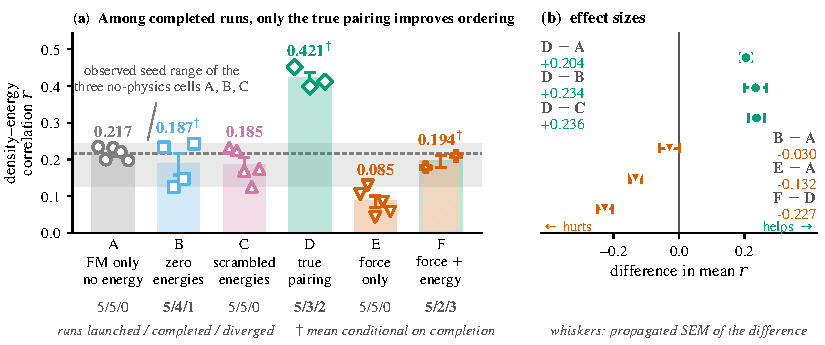
\includegraphics[width=\linewidth]{figures/out/fig3_grid.pdf}
\end{center}
\caption{Archived readout results; likelihood labels in the plots refer to $\widehat\ell_\theta$, not a validated generator density. \textbf{A matched six-cell grid isolates what the energy term
contributes.} Population: 120 held-out parents, reference geometry dropped, 8
displaced geometries each, scored by an independent GFN2-xTB evaluator, not the
eSEN training teacher. Metric: the per-parent density--energy correlation $r$,
per cell as the mean over completed training seeds (whisker: standard error
over seeds) with every completed seed drawn, and in (b) as effect sizes:
differences of cell means, whiskers the propagated descriptive SEM of the
difference rather than a confidence interval. Cells A--F are defined in
\Cref{sec:ablation}; runs launched / completed / diverged are printed under each
cell, because completion is objective-dependent. Only the true geometry--energy
pairing separates: every completed D seed lies above the shaded band, the
observed seed range of A, B and C; the zero-energy and scrambled cells do not,
and the gradient baseline falls below. \textbf{Cells B, D and F lost seeds to divergence}
($\dagger$), so their means are conditional on completion and the D and F
unconditional magnitudes are not identified. Panel detail in
\Cref{app:figdetail}.}
\label{fig:grid}
\end{figure}


\textbf{The gradient comparator.} Cell E carries the score-matched force term alone, completed $5/5$
at $0.085 \pm 0.016$, below the physics-free baseline by $-0.132$; added to the value term it
subtracts again, F scoring $0.194 \pm 0.016$ against D's $0.421$, a difference of $-0.227$. Cell E2,
identical to E at $\lambda_1 = 0.01$, completed $5/5$ at $0.080 \pm 0.013$, so the result does not
rest on one badly chosen weight (\Cref{app:p0cells}). The claim stays narrow. Under this implementation's endpoint
parameterisation these cells match a score equal to $(1-t)$ times \eqref{eq:score}
(\Cref{app:forcemech}); what is measured is that comparator --- naive, off-policy, endpoint --- on
this non-equilibrium corpus, and not \eqref{eq:score} at the scale it defines. It is not a claim that force supervision is unhelpful for
energy-grounded generation, which can be made to work \citep{psm,driftingboltzmann}; \Cref{prop:trap,prop:conflict}
name candidate mechanisms. Two forward-only diagnostics on the shared warm-start checkpoint locate
the difficulty: the endpoint force is a poor target at the interpolant, where the force actually
acting is nearly orthogonal to it (per-atom cosine $0.16$ at $t^{*} = 0.85$) because the
interpolant sits off the data manifold, and the force term's parameter gradient points
systematically against the flow-matching gradient while the value term's is close to orthogonal to
it. We read these as a measured mechanism for the observed difference rather than a proof
(\Cref{app:forcemech}).

\textbf{Completion by cell.} The launch record is A $5/5/0$, B $5/4/1$, C $5/5/0$, D $5/3/2$, E
$5/5/0$, F $5/2/3$ launched / completed / diverged: none of the ten runs without the value term
failed, against six of the twenty carrying it, cell B included, which implicates the reverse-time
log-density objective and its gradient rather than the teacher's energies; D and F are means over
survivors. Two records bound that risk. A later, byte-identically configured block of four cell-D
seeds completed in full at $0.353$, $0.374$, $0.452$ and $0.471$, and across all seven scored D runs
the mean is $0.416 \pm 0.017$; that block is reported separately and never merged into the grid
means. The F campaign launched $10$, completed $3$ and diverged $7$, its three completed runs
agreeing at $0.197 \pm 0.009$ (\Cref{app:p0cells,app:stability}).

\subsection{The Gain Generalises to Held-out Molecules and Retrieval}
\label{sec:mainresult}
\label{sec:main}
\label{sec:reference}

\textbf{Ordering improves well beyond seed spread.} On the conservative held-out endpoint ---
$93$ parents disjoint from the supervision pool, data geometry dropped, every geometry scored by the
independent evaluator --- the value term raises the mean per-parent correlation between
$\log q_\theta$ and $-E/kT$ from $0.200 \pm 0.018$ over five flow-matching seeds to
$0.369 \pm 0.023$ over four completed value seeds, an effect size of $\Delta r = +0.169$
(\Cref{fig:ordering}a). All four value seeds exceed all five control seeds, so the observed seed
ranges of the two arms do not overlap. The launch record is $5/5/0$ for flow matching and $5/4/1$
for the value arm, so the value mean is conditional on four of five completed launches, and
\Cref{app:imputation} reports conservative imputations for that run. The shift is spread across
the population rather than carried by a few parents, value supervision scoring higher on $67$ of the
$93$ (\Cref{fig:ordering}b).

\textbf{Retrieval improves, and the gain persists at fixed RMSD.} Ranking a parent's eight
displaced geometries by $\log q_\theta$ identifies the lowest-energy one $29.6\%$ of
the time under value supervision against $20.2\%$ for the control, with $12.5\%$ at chance, and
top-3 rises from $49.5\%$ to $62.4\%$ against $37.5\%$ (\Cref{fig:ordering}c). Retrieval is
invariant to the per-group constant and to calibration. The gain also persists at fixed RMSD: on a family
holding the within-group displacement magnitude constant to numerical precision, value supervision
reaches $0.305$ against $0.182$, a gap of $+0.124$ with four seeds per arm (\Cref{fig:ordering}d),
which rules out radial-distance variation as the sole explanation. A normal-mode family also has a
positive mean gap ($+0.185$ over five seeds per arm), but its observed seed ranges overlap, so we
treat it as supporting context only (\Cref{app:perturb}).

% figures/fig2_ordering.tex -- float wrapper for the held-out ordering figure
% (FIGURE 3 in the rendered PDF; cited as \Cref{fig:ordering} from Sec. 5.2).
% Image produced by figures/fig2_ordering.py, which also writes
% figures/out/fig2_ordering_data.json recording every plotted number and the
% file it came from.
%
% NOTATION.  Every drawn label reads \log q_\theta, the clamped positional-flow
% density (endpoint discrete labels held fixed, positional ODE reversed).  It is
% not the joint generator's conditional density and the caption says which
% quantity it is.  The stored record files keep the column name log_p_theta;
% that is a data-file field name and is never drawn.
%
% PROVENANCE
%   panel (a)  figures/out/scale_primary.json, ["dropref"][arm]["per_seed"]
%              [seed]["primary_93"]["pearson_r"], cross-checked at build time
%              against runs/eval_ours/wide_*/boltz_records.csv (both routes
%              agree to 4 decimals; the generator asserts it).
%   panel (b)  runs/eval_ours/wide_*/boltz_records.csv, pert_id 0 dropped,
%              restricted to the 93 ids in figures/out/primary_endpoint.json.
%   panel (c)  figures/out/retrieval_utility.json, ["primary_93"] blocks.  The
%              file's ["oracle"] key is renamed on load: the quantity is the
%              independent evaluator scoring the eSEN TRAINING TEACHER, i.e. an
%              ensemble-specific teacher-evaluator agreement reference, and that is what
%              the legend says.  Its numeral is not printed in the figure.
%   panel (d)  Gaussian side: the same records as (a).  Fixed-RMSD side: the
%              verified pair (value 0.305, flow matching 0.182, gap +0.124,
%              four seeds per arm) carried as constants in the generator.
%              See the ruling below.
%
% RULINGS HONOURED
%   * PANEL (d) IS DRAWN, AND ITS LIMIT IS DRAWN WITH IT.  No artefact under
%     runs/eval_p3 reproduces the verified fixed-RMSD aggregation -- the __cpu
%     round (40 parents, 4 seeds/arm) gives 0.3028 / 0.1885 and the __gpu60
%     round (120 parents, 4 seeds/arm) 0.3505 / 0.2482 -- so the panel plots the
%     verified ARM MEANS ONLY, prints the seed count, draws no per-seed cloud on
%     that side, and says in the panel that the two families are separate rounds
%     on different parent sets and that the comparison is between the gaps.
%     Splicing another round's per-seed cloud under the verified means would be
%     a cross-round comparison and is not done.
%   * The standardised geometry-level scatter that used to be panel (c) is
%     REMOVED.  Its fitted coefficient was algebraically the panel-(a) arm mean,
%     so it restated a number two other panels already carried, and the
%     fixed-RMSD control answers a claim-threatening confound that no other
%     panel addresses.
%   * The scrambled-energy arm is REMOVED from panel (a): only one of its two
%     shards was scrambled, so it is defective, and cell C of \Cref{fig:grid}
%     supersedes it.  No number that the verified register does not carry is
%     drawn anywhere in this figure.
%   * Every arm with three to five seeds shows its raw seed points -- panels
%     (a), (c) and the Gaussian half of (d).
%   * Every "ceiling" and "oracle" label is gone.  The orange marker in panel
%     (c) is the teacher-evaluator agreement reference, labelled ensemble-specific.
%   * NO INFERENTIAL STATISTIC IS DRAWN.  The reporting standard is descriptive:
%     arm means over independently trained seeds, the standard error over those
%     seeds, every raw seed point, the absolute gain Delta r, the seed counts,
%     and the launched/completed/diverged record.  The Welch t and the exact
%     permutation p are still computed as pipeline guards and are written to
%     figures/out/fig2_ordering_data.json, but no t value, no p-value and no
%     significance label reaches the image or the caption.
%   * Palette semantics are the fixed ones: grey = FM-only baseline,
%     green = value/energy.  Vermilion (force) does not appear -- the
%     gradient-supervision baseline is argued in Sec. 5.3.
%   * WIDTH.  This float places the PDF at \linewidth = 5.50 in and the
%     generator DRAWS at 5.50 in (FULL_W = PLACED_FRACTION * TEXTWIDTH_IN with
%     PLACED_FRACTION = 1.00), so the scale on the page is 1.000 and every
%     in-figure point size is a true page point size, none below 7 pt.  An
%     earlier 0.76 placement of a 5.5 in canvas shrank every size to 76% of
%     what the generator asked for; do not go back to it.  Do not \resizebox
%     this float, and if the placement here ever changes, change
%     PLACED_FRACTION in the generator to match.
\begin{figure}[t]
\begin{center}
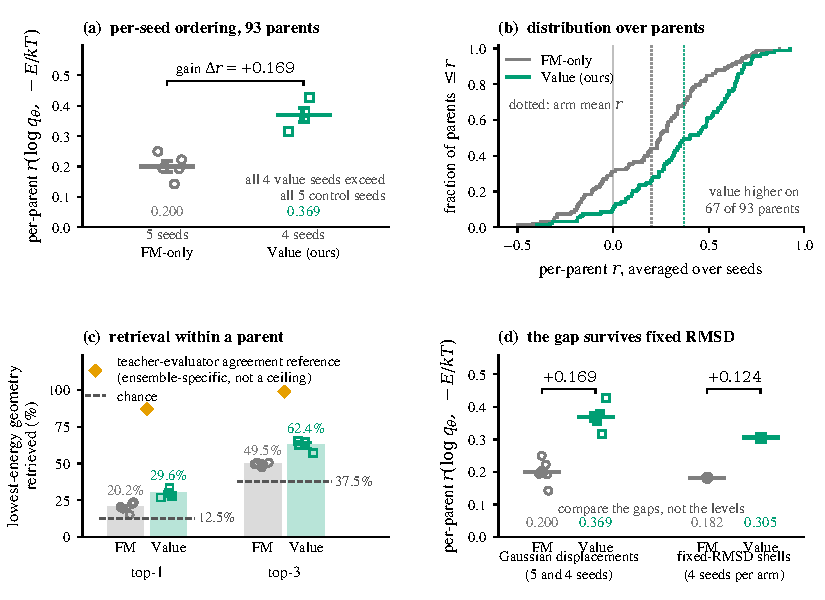
\includegraphics[width=\linewidth]{figures/out/fig2_ordering.pdf}
\end{center}
\caption{Archived readout results; likelihood labels in the plots refer to $\widehat\ell_\theta$, not a validated generator density. \textbf{Energy-value supervision improves local density--energy ordering.}
Population for \textbf{(a)}--\textbf{(c)}: the 93 held-out parents disjoint from the value term's
shard pool, data geometry dropped, up to eight displaced geometries each, scored by GFN2-xTB, an
evaluator independent of the eSEN potential that supplied the training energies. The metric is the
per-parent correlation between the clamped positional-flow density $\log q_\theta$ and $-E/kT$.
\textbf{(a)} Every seed of both arms; rules are arm means, bars their standard error over seeds,
and the gain is $\Delta r = +0.169$ with all four value seeds above all five control seeds. The
value arm is $5/4/1$ launched / completed / diverged, so its mean is conditional on completion.
\textbf{(b)} The shift is spread across the population rather than carried by a few parents.
\textbf{(c)} Ranking a parent's geometries by $\log q_\theta$ retrieves the lowest-energy one more
often; the orange marker is the teacher-evaluator agreement reference (not a ceiling): that
evaluator scoring the training teacher, ensemble-specific and re-measured for any other ensemble.
\textbf{(d)} Holding the within-group displacement magnitude constant to numerical precision leaves
the gap in place, so distance variation is not sufficient to explain the gain; that family is a
separate evaluation round on its own parents with four seeds per arm, and only its arm means are
plotted, so the comparison to make is between the two gaps, not between the two levels. Panel detail in \Cref{app:figdetail}.}
\label{fig:ordering}
\end{figure}


\textbf{Where the level sits.} Teacher and evaluator are different theories of chemistry, so a model
reproducing its teacher exactly would not score $1$: pushing the \emph{teacher's own} energies
through the identical pipeline gives $r = 0.927$ on the same 93 parents, an ensemble-specific
reference, not a ceiling (\Cref{app:scalediag}). Budget and locality remain open explanations of the
rest.

\subsection{Value Supervision Improves Ordering Before Calibration}
\label{sec:scale}

\textbf{Direction improves; the raw scale does not.} Ordering and calibration are different requests
of the same density, and the objective clearly answers the first. On the same models, seeds and
parents, the normalised residual variance rises from $1.402$ to $2.144$, where a \emph{constant}
log-density scores exactly $1$ (\Cref{fig:calibration}a): the arm that ranks geometries better sits
further from the Boltzmann scale, which is why we report the two quantities separately rather than
as one claim of physical grounding.

\textbf{The usable signal nonetheless increases.} No rescaling can bring a parent's
$\mathrm{NRV}_m$ below $1 - r_m^2$, and that optimally rescaled bound falls from $0.825$ to $0.747$
(\Cref{fig:calibration}b), so the density carries more energy-aligned information than before. The implied temperature moves the same way, from
$kT_{\mathrm{eff}} = 8.02$~eV to $2.34$~eV against the $1.0$~eV target (\Cref{fig:calibration}c),
and so does the slope, from $0.130$ to $0.448$: a response that was far too flat moves to the right
order of magnitude, overshooting rather than approaching. The same separation
appears against the eSEN training teacher, where $r$ rises from $0.202$ to $0.399$ while raw NRV
rises from $1.676$ to $2.821$ (\Cref{app:scalediag}).

\textbf{What is left is an optimisation gap, not a missing term.} Raw NRV additionally charges for
the part of the residual that is not energy-aligned, and that part grows enough to push NRV up even
as the rescaled bound falls; the free constant per group is not the cause, since $\mathrm{NRV}$ is
invariant to it. Both parts are already what \eqref{eq:lvalue} asks for. Writing
$\log q_\theta = a\,(-E/kT) + b + \varepsilon$ within a group, with $\varepsilon$ uncorrelated with
$E$ by construction, gives
\begin{equation}
  \Var_k\bigl(\log q_\theta + E/kT\bigr) \;=\; (a-1)^2\,\Var_k\bigl(E/kT\bigr) \;+\; \Var_k(\varepsilon),
  \label{eq:scaledecomp}
\end{equation}
whose two terms are exactly the magnitude of the response and its energy-unaligned component, and
which is minimised uniquely at $a = 1$ with $\Var_k(\varepsilon) = 0$. The variance form annihilates
the free constant $b$ but not the slope $a$: \eqref{eq:lvalue} already demands a calibrated
response, not merely a correctly ordered one. What we report is therefore not a term missing from
the objective but a gap between what it asks for and what this training run reached, and the
slope moving from $0.130$ to $0.448$ is movement along that axis rather than orthogonal to it. How far the slope can be driven by weighting the value term
more heavily, or by spending more of the budget on it, is a question these experiments leave open.\label{sec:generation}\ On generation itself we detect \emph{no
degradation in validity, PoseBusters pass rate \citep{posebusters} or uniqueness} at the evaluated
sample size (\Cref{app:generation}).

% figures/fig4_calibration.tex -- float wrapper for Figure 4 (Sec. 5.4).
% Image produced by figures/fig4_calibration.py, which also writes
% figures/out/fig4_calibration_data.json recording every plotted number and the
% file it came from.
%
% REVISION C6 (correctness fix, applied 2026-08-14)
%   The previous version overlaid the continuous curve NRV = 1 - r^2 on a plane
%   whose points are (mean-over-parents r, median-over-parents NRV).  That curve
%   is not a valid boundary for such an aggregate: the identity is per parent,
%   NRV_min(m) = 1 - r_m^2, and mean_m[1 - r_m^2] != 1 - (mean_m r_m)^2.  The
%   curve has been REMOVED.  The optimally rescaled bound is now reported the
%   only way it can be reported honestly, as its own per-seed aggregate, in the
%   new panel (b).  The generator asserts the per-parent identity at build time.
%   The teacher point is now labelled the TEACHER-EVALUATOR AGREEMENT REFERENCE
%   (the independent evaluator scoring the training teacher), never a ceiling.
%
% PROVENANCE (every number machine-read; nothing transcribed from prose or PDF)
%   all panels  figures/out/scale_primary.json, ["dropref"][arm]["per_seed"]
%               [seed]["primary_93"].  Panel (a) uses "pearson_r" (MEAN over the
%               93 parents) and "nrv" (MEDIAN over parents); panel (b) uses
%               "nrv" and "nrv_min" (MEAN over parents); panel (c) uses
%               "T_eff_eV" (kT divided by the median per-parent slope).
%               All four are cross-checked at build time against the per-parent
%               blocks of runs/eval_ours/calibration/calibration_dropref.json
%               restricted to the 93 ids in figures/out/primary_endpoint.json;
%               the two routes agree to 4 decimals and the generator asserts it.
%   reference   runs/eval_ours/ceiling_full_dropref/ceiling_per_group.csv,
%               restricted to the same 93 ids.  Its r = 0.9271 is the verified
%               number; its NRV = 0.082, NRV_min = 0.095 and kT_eff = 1.25 eV
%               were DERIVED for this figure from that file under the same
%               aggregation conventions as the model arms, and the caption says
%               so.
%
% RULINGS HONOURED
%   * No 1 - r^2 curve (revision C6).
%   * The three properties stay separated: this figure measures local ordering
%     and local calibration only.  Global mass allocation is not measured
%     anywhere in the paper and no panel here implies otherwise.
%   * Every arm shows its raw seed points: 4 open markers per arm in all three
%     panels (five for the flow-matching control), with the filled marker or rule
%     the arm mean over seeds and the
%     bar its standard error over seeds.
%   * The orange point is a reference, not a ceiling.  The figure labels it
%     "teacher-evaluator agreement" and prints its two numbers; what it is and is not is
%     stated in the caption, where it can be read at caption size.
%   * No p-value is printed here; the primary contrast statistics live with
%     Figure 2 and Table 1.
%   * Palette semantics are the fixed ones: grey = FM-only baseline,
%     green = value supervision, orange = teacher-evaluator agreement.
%     Vermilion (force) does not appear; the gradient-supervision baseline is
%     argued in Sec. 5.3.
%   * Drawn at final size (5.5 x 2.10 in) with an explicit, non-tight bounding
%     box; included with width=\linewidth, never rescaled.  Placed size equals
%     drawn size, so every in-figure point size is a page point size and nothing
%     renders below 7 pt.
%
% C12 (figure-editor pass, reviewer item 8).  The float placed this PDF at
% 0.76\linewidth while the canvas was drawn at 5.5 in, so in-figure type
% rendered at 76% of its stated size.  The placement is back to \linewidth and
% the canvas height is the height the float already occupied (2.72 x 0.76 =
% 2.067 in), so the vertical footprint is unchanged and the panels grow into the
% column width the fractional placement was wasting; panel (c) goes from 0.61 to
% 0.98 in wide.  The teacher-evaluator agreement annotation is cut to the two
% numbers, with what the point is and is not moved into the caption.  Every
% temperature label reads kT_eff, which is what the quantity is: an energy in
% eV, kT divided by the fitted slope, against a numerical kT = 1.0 eV target.
\begin{figure}[t]
\begin{center}
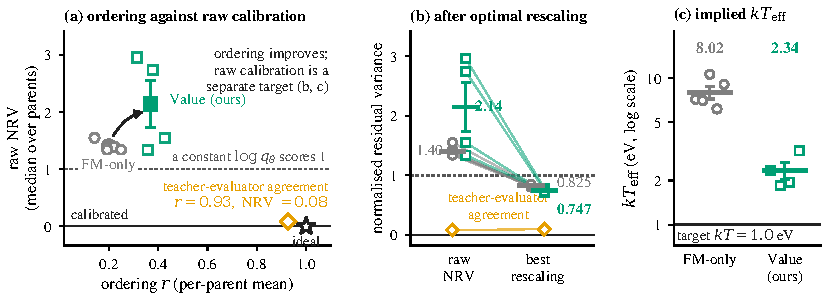
\includegraphics[width=\linewidth]{figures/out/fig4_calibration.pdf}
\end{center}
\caption{Archived readout results; likelihood labels in the plots refer to $\widehat\ell_\theta$, not a validated generator density. \textbf{Value supervision improves ordering before calibration.}
Same 93 held-out parents as \Cref{fig:ordering}, reference geometry dropped, GFN2-xTB evaluator;
five seeds for the flow-matching control, four for the value arm (open markers; filled marker or
rule the arm mean, bar its standard error over seeds). Metrics: ordering $r$ against raw
calibration $\mathrm{NRV} = \mathrm{Var}(\log q_\theta + E/kT)/\mathrm{Var}(E/kT)$ \textbf{(a)},
the optimally rescaled residual $\mathrm{NRV}_{\min}$ \textbf{(b)}, and the implied
$kT_{\mathrm{eff}}$ \textbf{(c)}. Three diagnostics move toward the Boltzmann-consistent regime:
$r$ rises from $0.200$ to $0.369$, $\mathrm{NRV}_{\min}$ falls from $0.825$ to $0.747$, and
$kT_{\mathrm{eff}}$ moves from $8.02$ to $2.34$~eV toward the $kT = 1.0$~eV target. Raw residual
variance --- the diagnostic most directly aligned with the objective as displayed --- remains a
separate unmet target: NRV rises from $1.402$ to $2.144$, past the $1$ that a constant
log-density scores, showing that errors in response magnitude and energy-unaligned variation
remain even as ordering improves. The value arm ($5/4/1$ launched / completed / diverged) is
conditional on completion. The orange marker is the teacher-evaluator agreement reference (not a
ceiling); panel detail and its derivation are in \Cref{app:figdetail}.}
\label{fig:calibration}
\end{figure}



% --- Sec. 5 Conclusion, with the compressed limitations folded in.
\section{Conclusion and Remaining Requirements}
\label{sec:limitations}
\label{sec:conclusion}
Group-wise energy values improve a legacy scalar ordering diagnostic in the archived molecular
experiments. They have not yet been shown to improve the generator's density or its samples.
The readout's endpoint/velocity mismatch, incomplete likelihood gradient, solver sensitivity and
uncalibrated energy response prevent a Boltzmann-sampling claim. The generation-strain experiment
adds no positive evidence, and many optimisations do not converge.

The corrected clamped-flow implementation supplies a testable next experiment. It still requires
matched training across seeds, exact/probe-repeat and resolution checks, an untouched test set, a
properly specified force baseline, and generation outcomes reported with all failures. Group-overlap
theory constrains an ideal residual on the supervised support; it neither repairs an invalid
likelihood nor predicts performance of the implemented update. These distinctions must be resolved
before presenting this intervention as a reliable molecular sampling method.


% --- Optional, unnumbered.  Keep commented until camera-ready: funding
%     acknowledgements go here and nowhere else.
%\subsubsection*{Author Contributions}
%\subsubsection*{Acknowledgments}

% --- main text ends here.  The three statements below sit after it and are
%     off the 9-page budget, so the label that build.sh measures precedes them.
\label{endofmaintext}

% ===========================================================================
%  FRONT-MATTER STATEMENTS.  These sit after the main text and are off the
%  9-page budget.  Unnumbered \subsubsection* blocks, per the template.
% ===========================================================================

\subsubsection*{Statement on the use of large language models}

Generative AI tools were used throughout the preparation of this work. They assisted
with software implementation and debugging, plotting, construction of the
result inventory, literature organisation, manuscript structuring and language
editing, and they provided feedback on experimental design and interpretation and help
in drafting the mathematical exposition. The authors selected the research questions
and the final methodology, executed or supervised every experiment, inspected the
per-run records, are responsible for verifying the final reported numbers, mathematical statements,
citations and AI-assisted text. This working revision includes an implementation audit;
it does not assert that all historical claims have been independently certified. The authors take responsibility for the complete manuscript and for the
accompanying artifacts.

\subsubsection*{Reproducibility statement}

\emph{What the paper specifies.} The objective is stated in full in \Cref{sec:method}
(\eqref{eq:ffjord}, \eqref{eq:lvalue}), and the gradient actually taken through it --- a
frozen-trajectory surrogate rather than differentiation through the solve --- is written out in
\Cref{app:asimplemented}. The standing assumptions and the complete proofs behind
\Cref{prop:ident}, in particular \Cref{thm:l2g} and \Cref{cor:basins}, are in \Cref{app:proofs}.
The backbone, optimiser, schedule, objective weights, warm-up and ramp, clipping thresholds, probe
times and estimator settings are tabulated in \Cref{app:hyper,app:constants}; the training scale and
hardware are in \Cref{app:hardware}; data preprocessing and the construction of the perturbation
shards, including which shards each arm reads, are in \Cref{app:data}. The evaluation protocol, the
independent scorer, the primary-endpoint construction and the aggregation rules are in
\Cref{app:eval,app:scalediag}, which also state the reporting policy --- effect sizes, arm means with
standard errors over independently trained seeds, and every seed-level result --- and which give the
adverse imputation for the one unreported run. The inferential statistics computed
during the analysis are collected once, for completeness and in one place, in
\Cref{app:inferential}. The complete launch record, including every run that diverged, every run that
completed without being scored, and the later seeds launched outside the matched design, is in
\Cref{app:p0cells,app:cells,app:stability}, and \Cref{app:allevals} inventories every evaluation we
ran, scored or not. \Cref{app:figdetail} states how each main-text figure panel was constructed from
those records.

\emph{What the displayed commands do and do not reproduce.} \Cref{app:repro} gives the two
environments, why they are separate, and the ordered command sequence. That sequence is exact for
one of the paper's two families of numbers and not for the other, and we state the difference
plainly. The matched six-cell grid of \Cref{sec:ablation} --- and hence \Cref{fig:grid} and the
per-seed tables of \Cref{app:p0cells} --- follows from the commands as displayed: perturbation
shards drawn from the training split alone, $M = 8$ parents per value step, value-loss cap $1500$.
The primary held-out endpoint of \Cref{sec:mainresult,sec:scale} does \emph{not}: those checkpoints
come from an earlier family trained under the archived configurations described in
\Cref{app:cells}, whose shard list also contains a validation-split shard, with $M = 4$ parents per
value step and a value-loss cap of $3000$, evaluated on $120$ parents and then restricted by the
disjoint-parent filter to the $93$ reported. Reproducing that endpoint therefore means training from
those archived configurations rather than from the matched-grid ones; running the displayed training
commands and applying the endpoint analysis would reproduce the protocol but not the checkpoints.
\Cref{app:cells} records that family's configuration defects and states which of its contrasts
survive the corrections and which are superseded by the matched grid.

\emph{Two caveats a re-runner should expect.} Diverged runs are recorded rather than re-rolled, and
because divergence is objective-dependent, every value-cell mean is reported conditional on
completion with its launched, completed and diverged counts beside it (\Cref{app:stability});
a re-run at a different seed set should expect a different completion pattern. The archived main-text comparisons use the legacy scalar readout, which the audit finds is not a
validated likelihood: it integrates an endpoint head as a velocity and freezes the numerical
trajectory in its gradient. The corrected $q_T$ coordinate flow is a separately defined sampler,
trained and diagnosed only in the development experiments of \Cref{app:newdevelopment}.
Numbers from these implementations must not be pooled or described as one likelihood protocol.

\subsubsection*{Ethics statement}

This work trains a generative model of small molecules against a
publicly released quantum-chemistry corpus and a publicly released neural
potential, and evaluates it with an open-source semi-empirical method; no human
subjects, personal data or human annotation are involved. De novo molecular
generators carry a dual-use risk in common with the rest of this literature, in
that a method for proposing molecules with desired properties could in
principle be directed at harmful ones. The models reported here are trained for
approximately $0.12$ epochs, are not conditioned on any biological or
toxicological objective, and generate chemically valid structures at a rate
well below what a practical design pipeline would require, so we judge the
incremental risk of this particular study to be low. The scientific claims are
deliberately bounded: we report a local ordering result, report calibration and
global mass allocation as separate and unmet targets, and \Cref{sec:limitations}
states what the paper does not establish.

\bibliography{refs}
\bibliographystyle{iclr2027_conference}

% ===========================================================================
\appendix
% Restart the float counters in the appendix and prefix them with the section
% letter, so appendix floats print as "Table A1", "Figure A1", ...
\setcounter{table}{0}
\setcounter{figure}{0}
\renewcommand{\thetable}{A\arabic{table}}
\renewcommand{\thefigure}{A\arabic{figure}}
% ============================================================================
%  sections/A1_proofs.tex --- Appendix A: theory.
%
%  Organisation.  One subsection per object:
%    A.1  setup, notation, standing assumptions
%    A.2  the log-density estimator: change of variables, Hutchinson trace,
%         and the integration scheme (explicit Euler in the state, midpoint
%         quadrature for the divergence integral).  It targets log q at t=1
%         at EVERY step count; the step count controls accuracy, not target.
%    A.3  the flow-matching score read-out          (lem:score)
%    A.4  why the gradient condition is a trapped surrogate (prop:trap/conflict)
%    A.5  the value condition                       (thm:certificate, cor:gauge)
%    A.6  local-to-global identifiability           (thm:l2g, cor:basins)
%    A.7  the training objective as a surrogate for the metric (prop:surrogate)
%    A.8  scope of the theory
%
%  The force-gauge aside (lem:forcegauge / thm:gauge) was DELETED in the
%  2026-08-29 appendix-compression pass: no experiment exercised it, it was not
%  the explanation of the force result, and it was not a contribution.  Do not
%  re-add it.
%
%  Conventions that must not be reverted:
%    (1) free energy is A(c) = -kT log Z(c); F is ALWAYS the force.
%    (2) coordinates are x, never r.
%    (3) no ESS claim: we never measured ESS.
%    (4) the rigid-motion assumption is COM-removal only -- the code does NOT
%        quotient rotations.
%    (5) charge is threaded to the teacher, spin is not (singlet default).
%    (6) the L_value gradient is a frozen-trajectory / truncated-adjoint one,
%        so the theory is scoped to the zero set and identifiability of the
%        ideal residual condition and NOT to convergence of that update.
%    (7) the reported density is the CLAMPED POSITIONAL-FLOW density q_theta;
%        p_theta is reserved for the joint generator's conditional density and
%        appears only in ass:A2's contrast clause.
%
%  REPEATED CAVEATS ARE CONSOLIDATED.  Each of the following is stated once in
%  the main text and once here, at the anchor named, and is cross-referenced
%  rather than restated: q_theta is not the joint conditional (ass:A2); the
%  divergence is prior work (rem:logvar); the implemented gradient is a
%  truncated-adjoint surrogate (rem:idealresidual); the objective is local and
%  does not identify basin mass (cor:basins); kT = 1 eV is numerical
%  (app:hyper); the likelihood estimate is resolution-dependent (ass:A-disc,
%  app:estimator); value-arm means are conditional on completion (app:p0cells).
%
%  Theorem environments are declared in main.tex and the counters continue from
%  the main text, so appendix-only results start after Theorem 1 / Lemma 1 /
%  Corollary 1.  Proofs of main-text results use
%  \begin{proof}[Proof of \Cref{...}] and introduce no second numbering.
% ============================================================================

\section{Theory: Assumptions, Estimator, and Proofs}
\label{app:proofs}

This appendix collects everything the main text states without proof, in the order
the argument uses it: the standing assumptions (\Cref{app:setup}); what the
reported log-density actually is, derived from the flow (\Cref{app:density}); the
score read-out the gradient baseline relies on and the two reasons it is a poor
target (\Cref{app:score,app:trap}); the certificate behind the value objective and
exactly what it identifies (\Cref{app:certificate,app:l2g}); the identity linking
the training objective to the reported metric (\Cref{app:surrogate}); and a closing
inventory of which statements this paper exercises and which it only states
(\Cref{app:scope}).

\subsection{Setup, notation and standing assumptions}
\label{app:setup}

A molecular state is a pair $(c,\vx)$. Operationally the composition $c \in \mathcal{C}$ is the
element multiset with the atom count $N(c)$ it determines and the total charge
$q$, which is what the pipeline threads to the teacher, and $\mathcal{C}$ is
countable. Spin multiplicity $s$ is a standing restriction rather than a
component of $c$: it is never passed and the teacher defaults to a singlet
(\Cref{ass:charge}), so every statement below is at that default and the
composition audit used for identifiability keys on (element multiset, charge)
accordingly. The conformation
$\vx \in \R^{3N(c)}$ is the nuclear coordinate vector with the centre of mass
removed, so the effective dimension is $d = 3(N-1)$. The teacher is a universal
neural potential $E : (c,\vx) \mapsto \R$ \citep{omol25,esen},
smooth in $\vx$, with conservative forces $F(c,\vx) = -\nabla_{\vx} E(c,\vx)$,
and $kT>0$ is a fixed temperature scale in eV. Throughout, $F$ denotes the
\emph{force} and never a free energy.

The target is the joint Boltzmann law and its two factors,
\begin{equation}
  \pi(c,\vx) = \frac{e^{-E(c,\vx)/kT}}{\mathcal{Z}},
  \qquad
  Z(c) = \int e^{-E(c,\vx)/kT}\,\mathrm{d}\vx,
  \qquad
  A(c) = -kT \log Z(c),
  \label{eq:app-targets}
\end{equation}
so that $\mathcal{Z} = \sum_{c} Z(c) = \sum_c e^{-A(c)/kT}$,
$\pi(c) = e^{-A(c)/kT}/\mathcal{Z}$ and
$\pi(\vx \mid c) = e^{-E(c,\vx)/kT}/Z(c)$. Neither $Z(c)$ nor $\mathcal{Z}$ is
ever formed. The generative model is a flow $\mathrm{d}\vx_t/\mathrm{d}t =
v_\theta(\vx_t,t)$ transporting $p_0 = \mathcal{N}(0,\sigma^2 I)$ on the
centre-of-mass-free subspace at $t=0$ to $q_\theta := q_1^\theta$ at $t=1$ with
the discrete channels clamped at their endpoint labels (\Cref{ass:A2}),
trained on the linear interpolant
$\vx_t = (1-t)\vx_0 + t\vx_1$ \citep{lipman2023flowmatching,liu2023rectifiedflow,%
albergo2023interpolants}.

\begin{assumption}[Teacher regularity]
\label{ass:A1}
$E(c,\cdot)$ is the teacher potential at fixed $(N,q,s)$ and is $C^1$ in $\vx$ on
a connected domain.
\end{assumption}

\begin{assumption}[Which density is reported: the clamped positional-flow density]
\label{ass:A2}
The quantity every theorem below is stated for, and every experiment reports as
$\log q_\theta(\cdot \mid c)$, is the log-density of the \emph{clamped
positional flow}: the flow obtained by holding the discrete channels --- atom
types, formal charges and the empty bond tensor --- at their endpoint labels
$(a_1, c_1, e_1)$ for the whole reverse trajectory, while only $\vx$ evolves.
That object is positive on the sampled support and normalised on the
centre-of-mass-free subspace by construction, being an exact change of variables
applied to a normalised Gaussian prior \citep{ffjord}, up to the discretisation of
\Cref{ass:A-disc}. It coincides with the generator's own joint conditional density
$p_\theta(\cdot \mid c)$ only if the discrete trajectory is determined by its
endpoint; the generator evolves types and charges through a continuous-time Markov
chain, so in general the two differ, we have not quantified the difference, and
this is recorded as a limitation (\Cref{app:limitations}). The symbol $q_\theta$ is
used nowhere else in this appendix.
\end{assumption}

\begin{assumption}[Translation-invariant velocity field]
\label{ass:A3}
$v_\theta$ is invariant to global translation, so the ambient $3N$-dimensional
trace of its Jacobian equals the intrinsic $3(N-1)$-dimensional one
(\Cref{app:density}). The centre-of-mass-removed equivariant field of the backbone
satisfies this. \textbf{Rotations are not quotiented}: the prior log-density uses
effective dimension $3(N-1)$, i.e.\ centre-of-mass removal only. We do not claim a
rotation-quotiented density.
\end{assumption}

\begin{assumption}[Discretised likelihood]
\label{ass:A-disc}
The reported $\log q_\theta$ is a discretised continuous-flow likelihood ---
explicit Euler in the state, midpoint-rule quadrature for the divergence integral,
with a stochastic trace estimator --- so it is a biased and noisy estimate of the
exact clamped positional-flow log-density. The step count controls that bias; it
does not change which density is estimated. Step counts and probe counts are in
\Cref{app:hyper}; the consequences are worked through in
\Cref{app:density,app:estimator}.
\end{assumption}

\begin{remark}[What the theory is scoped to, given the implemented gradient]
\label{rem:idealresidual}
The gradient actually back-propagated through $\Ls_{\mathrm{value}}$ is a
truncated-adjoint surrogate: the reverse trajectory is advanced without gradient
tracking, each state is detached before its divergence is taken, and the prior term
is computed from a detached endpoint, so the parameter gradient flows only through
the divergence evaluations (\Cref{app:asimplemented}). We do not differentiate
through the ODE solve, and the implemented update is therefore not exact
likelihood-gradient descent. Every statement in this appendix is accordingly scoped
to the \emph{zero set and identifiability} of the ideal residual condition
$w \equiv \mathrm{const}$ --- what a model that had driven the population objective
to zero would have been shown, and what that leaves free --- and to nothing about
whether, or to what, the implemented update converges.
\end{remark}

\begin{assumption}[Rigid-motion and symmetry factors]
\label{ass:rigid}
$Z(c)$ in \eqref{eq:app-targets} is an integral over $\R^{3N}$ and therefore
carries translational and rotational volume factors and a symmetry-number
correction. We take $Z(c)$ to be the configurational integral in the
centre-of-mass-removed space that the density estimator actually models; as noted
in \Cref{ass:A3}, rotations are \emph{not} quotiented by the implementation.
Within a parent group this is benign: all $K$ perturbations are small
displacements of one data geometry in one frame, so any rotational volume
factor is approximately constant within the group and cancels from the per-group
correlation, and is exactly annihilated by the within-parent variance loss. It is
\emph{not} benign for any comparison across groups or across separated basins,
which is one more reason we make none (\Cref{thm:l2g}).
\end{assumption}

\begin{assumption}[Well-posed conditional energy]
\label{ass:charge}
$E(c,\cdot)$ is the potential at fixed $(N,q,s)$, so the teacher must be queried
with the correct charge and spin. Our implementation decodes the total charge from
the frozen charge channel and passes it to the teacher; the spin multiplicity is
\emph{not} passed and the teacher defaults to a singlet. For radicals and
open-shell complexes this is the wrong electronic state. Every reported evaluation
is on main-group organic parents drawn from the held-out split, where the singlet
default is the standard assignment for closed-shell species; we have not verified
the multiplicity of every evaluated parent. The restriction is recorded as a
limitation (\Cref{app:limitations}) and is the reason no radical, open-shell or
transition-metal result is reported.
\end{assumption}

\subsection{The reported log-density: change of variables, trace estimation, and the integration scheme}
\label{app:density}

Everything the value objective constrains, and everything the calibration
diagnostics measure, is the number this subsection defines. It is derived in three
steps --- an exact identity, an unbiased estimator of the one expensive term in it,
and an integration scheme --- and the third step is the one that decides how
\emph{accurately} the density is reported, not which density it is.

\paragraph{Step 1: the instantaneous change of variables.} Let $\vx_t$ solve
$\mathrm{d}\vx_t/\mathrm{d}t = v_\theta(\vx_t,t)$ and let $p_t$ be the law of
$\vx_t$. Mass conservation is the continuity equation
$\partial_t p_t + \nabla\!\cdot(p_t v_\theta) = 0$. Expanding the divergence,
$\nabla\!\cdot(p_t v_\theta) = \nabla p_t \cdot v_\theta + p_t \nabla\!\cdot v_\theta$,
and dividing by $p_t > 0$,
\begin{equation}
  \partial_t \log p_t + v_\theta \cdot \nabla \log p_t
  \;=\; -\,\nabla\!\cdot v_\theta .
\end{equation}
The left-hand side is the material derivative of $\log p_t$ along a trajectory, so
\begin{equation}
  \frac{\mathrm{d}}{\mathrm{d}t}\,\log p_t(\vx_t)
  \;=\; -\,\nabla\!\cdot v_\theta(\vx_t,t) ,
  \label{eq:app-icv}
\end{equation}
the instantaneous change of variables underlying continuous normalising flows
\citep{ffjord}. Integrating \eqref{eq:app-icv} from $t=0$ to $t=1$ along the
trajectory that ends at $\vx_1$ and using $p_0 = \mathcal{N}(0,\sigma^2 I)$ gives
\eqref{eq:ffjord} of the main text,
\begin{equation}
  \log q_\theta(\vx_1 \mid c)
  \;=\; \log p_0(\vx_0) - \int_0^1 \nabla\!\cdot v_\theta(\vx_t,t)\,\mathrm{d}t ,
  \qquad
  \vx_0 = \vx_1 - \int_0^1 v_\theta(\vx_t,t)\,\mathrm{d}t .
  \label{eq:app-ffjord}
\end{equation}
In practice the trajectory is generated \emph{backwards} from the data point
$\vx_1$, so one reverse solve returns both $\vx_0$ and the accumulated divergence.
\Cref{eq:app-ffjord} is exact in continuous time and requires no invertibility
argument beyond uniqueness of the ODE solution; every approximation in the reported
number enters in steps 2 and 3.

\paragraph{Step 2: the trace, and why a stochastic estimator is used.} The
divergence is the trace of the Jacobian, $\nabla\!\cdot v_\theta = \operatorname{tr} J$
with $J_{ij} = \partial (v_\theta)_i/\partial x_j$. Computing $\operatorname{tr} J$ exactly
costs $3N$ backward passes, one per coordinate, at every integration step. The
Hutchinson estimator \citep{hutchinson} replaces it by
\begin{equation}
  \operatorname{tr} J \;=\; \E_{\epsilon}\bigl[\epsilon^{\!\top} J \epsilon\bigr],
  \qquad \E[\epsilon] = 0,\quad \E[\epsilon\epsilon^{\!\top}] = I ,
  \label{eq:app-hutch}
\end{equation}
which is exact in expectation for any such $\epsilon$, and each sample costs one
vector--Jacobian product --- a single backward pass --- followed by an inner product
with $\epsilon$. We use $n_{\mathrm{p}} = 2$ Rademacher probes per step, i.e.\ two
backward passes in place of $3N$.

Two properties of \eqref{eq:app-hutch} matter for how the resulting numbers may be
read. First, with independent entries the estimator's variance is
\begin{equation}
  \Var\bigl[\epsilon^{\!\top} J \epsilon\bigr]
  \;=\; \sum_{i<j} \bigl(J_{ij}+J_{ji}\bigr)^{2}
  \;\;\xrightarrow{\;J = J^{\!\top}\;}\;\;
  2\Bigl(\lVert J\rVert_F^{2} - \textstyle\sum_i J_{ii}^{2}\Bigr) ,
  \label{eq:app-hutchvar}
\end{equation}
because $\epsilon^{\!\top} J\epsilon = \sum_i J_{ii} + \sum_{i<j}(J_{ij}+J_{ji})\epsilon_i\epsilon_j$
and the products $\epsilon_i\epsilon_j$ over distinct pairs are uncorrelated with unit
variance. Rademacher probes are the standard choice because the diagonal of $J$
contributes no variance at all, whereas Gaussian probes pay $2\lVert J\rVert_F^2$;
averaging $n_{\mathrm{p}}$ probes divides \eqref{eq:app-hutchvar} by
$n_{\mathrm{p}}$. Second, the divergence enters \eqref{eq:app-ffjord}
\emph{linearly}, so trace noise adds variance to the reported $\log q_\theta$ but
no bias: an unbiased trace at every step gives an unbiased estimate of the
discretised integral. The bias in the reported number comes from the quadrature,
not from the probes. We have not measured the repeat-to-repeat spread of
$\log q_\theta$ on the reported population, and say so as a limitation
(\Cref{app:limitations}).

Finally, \Cref{ass:A3} is what lets the probes be drawn in the ambient $3N$
coordinates without correcting the dimension. If $v_\theta$ is invariant to a
global translation then $J u = 0$ for each of the three uniform-translation
directions $u$, so those directions contribute zero eigenvalues and the ambient
trace equals the trace of $J$ restricted to the centre-of-mass-free subspace.
Rotations enjoy no such identity and are not quotiented anywhere in the
implementation.

\paragraph{Step 3: the integration scheme, and what the step count does and does not
control.} The reverse-time solve of \eqref{eq:app-ffjord} uses \emph{explicit Euler
in the state with midpoint-rule quadrature for the divergence integral}. With $n$
steps the implementation sets $\Delta t = 1/n$ and evaluates the field and its
divergence at
\begin{equation}
  t_k \;=\; 1 - \Bigl(k + \tfrac{1}{2}\Bigr)\Delta t ,
  \qquad k = 0,1,\dots,n-1 ,
  \label{eq:app-grid}
\end{equation}
accumulating $-\Delta t\,\nabla\!\cdot v_\theta(\vx_{t_k},t_k)$, advancing the state
by $\vx \leftarrow \vx - \Delta t\, v_\theta(\vx,t_k)$, and adding the prior
log-density at the end.

Two schemes are in play and they must not be conflated. The \emph{state} update is
explicit Euler with $n$ steps of size $1/n$, which traverses the whole of $[0,1]$
and carries $O(\Delta t)$ error. The \emph{divergence} integral is approximated by
the midpoint rule on $[0,1]$: all $n$ nodes are interior to the interval, the
interval itself is not truncated, and the rule carries $O(\Delta t^{2})$ error and
is exact for integrands linear in $t$. The half-step offset therefore avoids
evaluating the field at $t = 1$ without moving the endpoint the scheme targets. For
every $n$, what the estimator targets is $\log q_\theta$ at $t = 1$; there is no
family of smoothed marginals indexed by the step count, and refining $n$ estimates
the \emph{same} quantity more accurately rather than a different one. Analytic
checks on the implementation confirm this: on a field of constant divergence, and on
a time-varying one, the accumulated integral equals the full-interval value at every
$n$ rather than a truncated $1 - 1/(2n)$ value, and on a linear continuous
normalising flow the estimate converges to the closed-form endpoint log-density as
$n$ grows.

Step-count dependence in the reported numbers is accordingly \emph{numerical
discretisation error}, dominated by the $O(\Delta t)$ Euler state integration rather
than by the $O(\Delta t^{2})$ quadrature, together with whatever endpoint stiffness
the learned field carries. \Cref{app:estimator} tabulates the step counts, reports
what the absence of a plateau looks like on real molecules, and measures how much of
the reported effect size depends on the choice.

Two uses of the symbol $\epsilon$ must be kept apart, and neither is a smoothing
scale of the reported density: the $\epsilon$ of \eqref{eq:app-eps} below is the
Gaussian width $(1-t)\sigma/t$ attached to the flow-matching score read-out at a
probe time $t$ and not to the likelihood estimator, and it is unrelated to the
mass-relaxation $\varepsilon$ of \Cref{rem:epsilon}, which is written with a
different glyph throughout.

\subsection{The flow-matching score read-out}
\label{app:score}

The gradient-supervision baseline of \Cref{sec:method} needs the score of the
model's own time-$t$ marginal. Flow matching supplies it in closed form, which is
convenient and, as \Cref{app:trap} shows, also the source of the baseline's
trouble.

\begin{lemma}[Flow-matching score read-out]
\label{lem:score}
Let $x_t = (1-t)x_0 + t x_1$ with $x_0 \sim \mathcal{N}(0,\sigma^2 I)$ independent of
$x_1 \sim p_{\mathrm{data}}$ and $v^{*}(x,t) = \E[x_1 - x_0 \mid x_t = x]$. Then for every
$t \in [0,1)$, $\nabla_x \log p_t(x) = \bigl(t\,v^{*}(x,t) - x\bigr)/\bigl((1-t)\sigma^2\bigr)$.
\end{lemma}

\begin{proof}[Proof of \Cref{lem:score}]
Conditionally on the data endpoint, $\vx_t \mid \vx_1 \sim
\mathcal{N}(t\vx_1, (1-t)^2\sigma^2 I)$, so the time-$t$ marginal
$p_t(\vx) = \int \mathcal{N}(\vx; t\vx_1, (1-t)^2\sigma^2 I)\,p_{\mathrm{data}}(\vx_1)
\,\mathrm{d}\vx_1$ is a Gaussian mixture with covariance independent of the
mixing variable. Differentiating under the integral sign and using
$\nabla_{\vx}\mathcal{N}(\vx;\mu,\Sigma) = -\Sigma^{-1}(\vx-\mu)\mathcal{N}$ gives
the posterior-mean form
\begin{equation}
  \nabla_{\vx}\log p_t(\vx)
  = \frac{t\,\E[\vx_1 \mid \vx_t = \vx] - \vx}{(1-t)^2\sigma^2}.
  \label{eq:app-mixture-score}
\end{equation}
The flow-matching regression target is $\vx_1 - \vx_0$, and
$\vx_0 = (\vx_t - t\vx_1)/(1-t)$ gives $\vx_1 - \vx_0 = (\vx_1 - \vx_t)/(1-t)$.
Taking conditional expectations, the marginal velocity is
$v^\ast(\vx,t) = (\E[\vx_1\mid \vx_t=\vx] - \vx)/(1-t)$, i.e.
$\E[\vx_1 \mid \vx_t = \vx] = \vx + (1-t)v^\ast(\vx,t)$. Substituting into
\eqref{eq:app-mixture-score}, one factor of $(1-t)$ cancels and
\begin{equation}
  s^\ast(\vx_t,t) \;=\; \frac{t\,v^\ast(\vx_t,t) - \vx_t}{(1-t)\sigma^2}.
  \label{eq:app-score}
\end{equation}
Replacing $v^\ast$ by the learned $v_\theta$ defines $s_\theta$. Finally, the map
$v \mapsto s$ in \eqref{eq:app-score} is affine with linear part
$t/((1-t)\sigma^2)$, so a velocity perturbation $\delta v$ moves the implied
score by $t\|\delta v\|/((1-t)\sigma^2)$.
\end{proof}

\begin{remark}[Sign]
\label{rem:sign}
Matching $s_\theta \to +F/kT$ is Boltzmann-attracting because
$\nabla_{\vx}\log \pi = -\nabla_{\vx}E/kT = +F/kT$. The sign in
\eqref{eq:app-score} is not a convention that may be flipped.
\end{remark}

\begin{remark}[Amplification at the probe times used]
\label{rem:app-amplification}
With $\sigma = 1$, the factor $t/((1-t)\sigma^2)$ equals $5.7$, $11.5$ and $32.3$
at the three training probe times $t \in \{0.85, 0.92, 0.97\}$. The pole at
$t = 1$ is not a removable artefact: $s_\theta$ is the score of the
\emph{smoothed} marginal $p_t$, and the smoothing vanishes exactly as the
read-off amplification diverges.
\end{remark}

\subsection{Why the gradient condition is a trapped surrogate}
\label{app:trap}

Two mechanisms, both specific to matching \eqref{eq:app-score} \emph{off-policy at
data endpoints}, are compatible with the gradient baseline failing to help. Both
turn on one structural fact: the network is a function of the interpolation state
$\vx_t$ while the target is the force read at the data endpoint $\vx_1$. Both are
stated as \emph{diagnostic hypotheses} rather than as explanations of the
measurement in \Cref{sec:ablation}; neither is isolated experimentally, and neither
bears on force supervision in general \citep{psm,driftingboltzmann}.

\begin{proposition}[Bias--variance trap: a diagnostic hypothesis]
\label{prop:trap}
At the population optimum of $\Ls_{\mathrm{FM}}$, and with
$\epsilon = (1-t)\sigma/t$, the read-out is, up to a factor $1/t$, the score of
$p_{\mathrm{data}} * \mathcal{N}(0,\epsilon^2 I)$ evaluated at
$\vx_1 + \epsilon z$, $z \sim \mathcal{N}(0,I)$. Compared with the endpoint target
$F(\vx_1)/kT$ this incurs a scale error and a smoothing error, each $O(1-t)$ or
smaller, together with an evaluation-point displacement of size $\epsilon$, while
by \Cref{rem:app-amplification} the gradient noise injected into the parameters
grows as $(1-t)^{-2}$. No choice of $t$ makes the deterministic terms and the noise
term small together.
\end{proposition}

\begin{proposition}[Objective conflict: a diagnostic hypothesis]
\label{prop:conflict}
The population minimiser of $\Ls_{\mathrm{FM}}$ has implied score
$\nabla \log p^{\mathrm{data}}_t(\vx_t)$. The network input is $\vx_t$ while the
force target is the endpoint quantity $F(c,\vx_1)/kT = \nabla\log\pi(\vx_1)$, so the
population minimiser of the idealised \emph{squared} off-policy force loss is not
$\nabla\log\pi(\vx_1)$ but the conditional expectation
\begin{equation}
  s_\theta(\vx_t,t) \;\longrightarrow\;
  \E\bigl[\nabla\log\pi(\vx_1) \bigm| \vx_t, t, c\bigr]
  \;=\; \E\bigl[F(c,\vx_1)/kT \bigm| \vx_t, t, c\bigr],
  \label{eq:app-condexp}
\end{equation}
a smoothed and shrunk field. The two population targets differ whenever the corpus
is not drawn from the target law, $p_{\mathrm{data}} \neq \pi$, and the joint
minimiser is neither; a fixed $\lambda_1$ moreover weights the conflicting target
by $(1-t)^{-2}$.
\end{proposition}

\begin{proof}[Proof of \Cref{prop:trap} and \Cref{prop:conflict}]
Reparameterise the smoothing. Write $\vx_t = t\,y$ with
\begin{equation}
  y = \vx_1 + \epsilon z, \qquad z \sim \mathcal{N}(0,I), \qquad
  \epsilon = (1-t)\sigma/t ,
  \label{eq:app-eps}
\end{equation}
so that $p_t(\vx) = t^{-d} \tilde p_\epsilon(\vx/t)$ with
$\tilde p_\epsilon = p_{\mathrm{data}} \ast \mathcal{N}(0,\epsilon^2 I)$, and
therefore $s_\theta(\vx_t,t) = t^{-1}\nabla\log\tilde p_\epsilon(\vx_1+\epsilon z)$
at the population optimum. Against the target $\nabla\log\pi(\vx_1)$ this exposes
four mismatches: a $1/t$ prefactor contributing relative error $(1-t)/t = O(1-t)$;
a smoothing error $\nabla\log(p \ast \mathcal{N}_\epsilon) - \nabla\log p =
O(\epsilon^2) = O((1-t)^2)$ by the heat-flow expansion; an evaluation-point
displacement contributing $\epsilon\,\nabla^2\log\pi\,z$ to first order; and, since
by \Cref{lem:score} any velocity error is multiplied by $t/((1-t)\sigma^2)$ and the
loss is quadratic in the score, parameter-gradient noise scaling as $(1-t)^{-2}$.
The first three shrink as $t \to 1$ while the fourth diverges, so the total error is
bounded below by a trade-off of the form $O(1-t) + O((1-t)^{-2}\eta)$ with $\eta$
the velocity-estimation noise level, which is \Cref{prop:trap}; averaging over
probe times, as we do, reduces the constant but not the trade-off.

For \Cref{prop:conflict}, the displacement is not merely noise that averages away.
The loss is minimised over functions of $\vx_t$, and $(\vx_t,\vx_1)$ are dependent
but not mutually determined, so for a squared loss the population minimiser over
measurable functions of the input is the conditional expectation
\eqref{eq:app-condexp}, by the orthogonality property of $L^2$ projection; it equals
$\nabla\log\pi(\vx_1)$ only if $\vx_1$ is $\sigma(\vx_t)$-measurable, which the
interpolation makes false for every $t < 1$. The result is a shrinkage \emph{bias}
in the learned score rather than a variance term, and the two population targets ---
the score of the data interpolation marginal, and the conditional expectation of
endpoint Boltzmann scores --- are distinct whenever $p_{\mathrm{data}} \neq \pi$.

Two caveats bound both propositions. The implemented $\ell$ is Huberised and
per-atom norm-capped \eqref{eq:score}, so its population minimiser is a robustified
location functional of the same conditional law and not \eqref{eq:app-condexp}. And
both arguments concern population objectives at their exact optima, so they name
mechanisms the construction admits rather than ones we have isolated.
\end{proof}

\begin{remark}[The antecedent holds for our data, and on-policy variants are outside what we measure]
\label{rem:antecedent}
The training corpus is a curated union of relaxation trajectories, molecular
dynamics snapshots and conformer sets across many systems, charges and spins
\citep{omol25}. It is not an equilibrium sample from a single-temperature Boltzmann
distribution, and the training $kT = 1.0$~eV is not a physical temperature of the
dataset, so the antecedent $p_{\mathrm{data}} \neq \pi$ of \Cref{prop:conflict}
holds by construction. Querying forces at model samples rather than at data points
would partially repair the evaluation-point displacement and the objective conflict,
because the two targets would then refer to one distribution; it would not repair
the $(1-t)^{-1}$ amplification. No such variant is measured here: the
gradient-supervision cells of the matched grid (\Cref{app:p0cells}) carry the
off-policy endpoint term alone, whereas the earlier round's force cells also carried
an on-policy distillation term, which is why that round's \emph{force} comparisons
are confounded and are superseded by cell E (\Cref{app:cells}).
\end{remark}

\subsection{The value condition: a partition-function-free certificate}
\label{app:certificate}

The certificate below is the standard zero-of-the-log-variance-divergence
statement written in our conditional notation. Its structural property --- that an
additive constant in $\log\tilde\pi$, hence the partition function, cancels --- is
due to the authors cited in \Cref{rem:logvar} and is not claimed here. We reproduce
the proof because \Cref{cor:gauge} and \Cref{thm:l2g} both refer to its internals.

\begin{theorem}[Zero-variance certificate on a region]
\label{thm:certificate}
Under the regularity assumptions of \Cref{app:setup} (smooth $E$, positive normalised
$q_\theta$ on the COM-removed subspace, translation-invariant velocity field), fix a composition
$c$, a region $U$ and a reference measure $\rho$ with $\mathrm{supp}\,\rho = U$, and let
$w(x) = \log q_\theta(x \mid c) + E(c,x)/kT$. Then \emph{(i)} $\Var_{x\sim\rho}[w] = 0$ if and
only if $w$ is $\rho$-a.s.\ constant on $U$; if $\rho$ has a positive Lebesgue density on $U$ this
says $q_\theta(\cdot \mid c)$ restricted to $U$ is proportional to $e^{-E(c,\cdot)/kT}$, and if
$\rho$ is atomic on $K$ sampled points it says $\log q_\theta$ and $-E/kT$ differ by one common
constant at those $K$ points, i.e.\ $K-1$ scalar equations, with no statement about points outside
the sample; \emph{(ii)} if $\rho$ has a positive Lebesgue density on $U$ then the multiplier is
fixed \emph{relative to $U$}, $a = q_\theta(U \mid c)/Z_U(c)$ with
$Z_U(c) = \int_U e^{-E(c,x)/kT}\,\mathrm{d}x$ the integral over $U$ and not the global $Z(c)$, so
that $q_\theta(\cdot \mid c, U) = \pi(\cdot \mid c, U)$ exactly; if in addition
$q_\theta(U \mid c) = 1$ then $a = 1/Z_U(c)$, and $q_\theta(\cdot \mid c) = \pi(\cdot \mid c)$
globally only when $U$ also carries all of the target's mass, $Z_U(c) = Z(c)$;
\emph{(iii)} $\Var_{x\sim\rho}[w]$ is
invariant to $E \mapsto E + g(c)$ and needs no evaluation of $Z(c)$ or $\mathcal{Z}$.
\end{theorem}

\begin{corollary}[What the empirical loss identifies]
\label{cor:gauge}
The empirical objective \eqref{eq:lvalue} has null space exactly the functions that are
constant within each parent group. It therefore determines $\log q_\theta(\cdot \mid c)$ up to
one free additive constant \emph{per group}, and no further.
\end{corollary}

\begin{remark}[Attribution]
\label{rem:logvar}
$\Var_\rho[w]$ with $w = \log q_\theta - \log\tilde\pi$ and
$\tilde\pi = e^{-E/kT}$ is the log-variance divergence \citep{vargrad,
nusken2021pathspace,richter2024improvedsampling}. Part (iii) --- invariance to
an additive constant in $\log\tilde\pi$, hence no partition function --- is the
defining structural property of that divergence and is due to those authors, not
to this paper. Estimating it under a reference measure that is not the model's own
(off-policy) is likewise standard \citep{nusken2021pathspace,sendera2024offpolicy}.
\end{remark}

\begin{remark}[The certificate is about the exact clamped density; what is formed is its discretisation]
\label{rem:epscert}
\Cref{thm:certificate} is stated for the exact normalised $q_\theta$, whereas what
the objective and the metric both form is its Euler/midpoint estimate at a finite
step count (\Cref{app:density}). The residual the objective can enforce therefore
carries discretisation bias, which does not vanish at the step counts we can afford
(\Cref{app:estimator}); the target quantity is the same at every step count, and the
accuracy is not.
\end{remark}

\begin{proof}[Proof of \Cref{thm:certificate}]
Fix $c$, a region $U$ and $\rho$ with $\mathrm{supp}\,\rho = U$; let
$w(\vx) = \log q_\theta(\vx\mid c) + E(c,\vx)/kT$.

(i) A random variable has zero variance if and only if it is a.s.\ constant, so
$\Var_{\vx\sim\rho}[w] = 0$ iff $w \equiv \kappa$ $\rho$-a.s.\ on $U$, and then
$q_\theta(\vx\mid c) = a\,e^{-E(c,\vx)/kT}$ with the positive multiplier
$a = e^{\kappa}$, for $\rho$-almost every $\vx \in U$. Note the sign: the residual
constant enters the density through $e^{+\kappa}$, and the same holds component by
component in \Cref{thm:l2g}. The strength of that conclusion depends on $\rho$. If $\rho$ has a
positive Lebesgue density on $U$, the identity holds Lebesgue-almost everywhere on
$U$ and $q_\theta$ restricted to $U$ is proportional to the Gibbs weight. If
$\rho$ is the empirical measure on $K$ sampled points, the identity holds at those
$K$ points and nowhere else is constrained: the certificate is $K-1$ scalar
equations, not a density statement, and asserting proportionality on a region from
finitely many pointwise equations would be a strictly stronger claim than the
variance supplies. Conversely if $q_\theta(\cdot\mid c) \propto e^{-E(c,\cdot)/kT}$
$\rho$-a.e.\ on $U$ then $w$ is constant there. Note that (i) alone is a statement
\emph{about $U$}: nothing outside $U$ is constrained.

(ii) Let $\rho$ have a positive Lebesgue density on $U$, so that (i) gives the
identity Lebesgue-a.e.\ on $U$ with a positive multiplier $a = e^{\kappa}$. Since
$q_\theta(\cdot\mid c)$ is a normalised density (\Cref{ass:A2}), integrating
$a\,e^{-E/kT}$ over $U$ gives $q_\theta(U \mid c) = a\,Z_U(c)$, where
$Z_U(c) = \int_U e^{-E(c,\vx)/kT}\,\mathrm{d}\vx$ is the integral over $U$ and
\emph{not} the global $Z(c)$. Hence $a = q_\theta(U\mid c)/Z_U(c)$, and dividing,
the conditional law is pinned exactly:
$q_\theta(\vx \mid c, U) = e^{-E(c,\vx)/kT}/Z_U(c) = \pi(\vx \mid c, U)$. Suppose in
addition $q_\theta(U\mid c) = 1$, so that $a = 1/Z_U(c)$: this determines the
multiplier but identifies $q_\theta(\cdot\mid c)$ with $\pi(\cdot\mid c)$
\emph{globally} only when the target also puts all of its mass on $U$, that is when
$Z_U(c) = Z(c)$. Otherwise the model is the Gibbs law truncated to $U$ and
renormalised, differing from $\pi(\cdot\mid c)$ by the factor $Z(c)/Z_U(c)$ on $U$
and by all of $\pi(U^{\mathrm{c}}\mid c)$ outside it. It is exactly the proviso
$q_\theta(U\mid c) = 1$ that our per-parent perturbation groups violate, which is
what \Cref{thm:l2g} quantifies, and even where it holds the step to a global
statement needs the target's mass to sit on $U$ as well. For an atomic $\rho$ no
hypothesis of this form is available at all: a finite point set is Lebesgue-null,
so $q_\theta(U \mid c) = 0$ for any continuous model density and part (ii) is
inapplicable rather than merely unattainable. The $\varepsilon$-relaxation of
\Cref{rem:epsilon} repairs mass leaking outside a bounded region but not a
Lebesgue-null reference measure, and we make no part-(ii) claim in the empirical
reading at any $\varepsilon$.

(iii) $\Var_{\vx\sim\rho}[w]$ is unchanged by $E \mapsto E + g(c)$ for any
function $g$ of composition alone, because such a shift adds a constant to $w$
within the group; and it involves neither $Z(c)$ nor $\mathcal{Z}$, because the
within-group centring subtracts whatever constant those would contribute
(\Cref{rem:logvar}).
\end{proof}

\begin{proof}[Proof of \Cref{cor:gauge}]
The empirical objective is
$\Ls_{\mathrm{value}} = M^{-1}\sum_{m}\Var_k(w_{m,k})$ with
$w_{m,k} = \log q_\theta(\vx_{m,k}) + E_{m,k}/kT$, where $m$ indexes parent
groups and $k$ indexes the $K$ perturbations of parent $m$. A within-group
variance is annihilated exactly by functions that are constant within each group
and by nothing else, so the null space of $\Ls_{\mathrm{value}}$ is the set of
per-\emph{group} additive constants --- one scalar $b_m$ per group, not one per
composition. The objective therefore determines the \emph{shape} of
$\log q_\theta$ inside each group's support and no more. Fixing those constants
requires absolute energies, which is the role of an anchor term; the anchor was
inactive in every run reported in this paper (\Cref{app:asimplemented}). One
granularity caveat belongs with that statement: the anchor as implemented predicts
its constant from element counts, atom count and total charge, so it is keyed on
the \emph{composition} and can fix at most one constant per composition, not the
one constant per group this corollary identifies. Those coincide only when a
composition supplies a single group, which our training pool does not satisfy for
$31\%$ of its parents (\Cref{app:data}).
\end{proof}

\subsection{Local-to-global identifiability}
\label{app:l2g}

\Cref{thm:l2g} characterises the null space of the group-wise objective under
stated support and normalisation assumptions; connectivity of the overlap graph is
what removes the per-component offsets from that null space. It does not decide
whether a trained model is Boltzmann, and no reported run has a connected overlap
graph. Because the statement is sensitive to the choice of reference measure, we
name ours first and then separate the continuous and the empirical readings.


% ---------------------------------------------------------------------------
%  RELOCATED FROM THE MAIN TEXT BY THE 2026-08-19 COMPRESSION PASS.
%  Sec. 4 of the main text now carries a single short proposition
%  (prop:ident); the full statements live here, immediately before their
%  proofs.  Text is verbatim from the pre-compression main text.
% ---------------------------------------------------------------------------

\begin{definition}[Overlap graph]
\label{def:overlap}
Fix a composition $c$ with groups $j = 1,\dots,J$ and reference measures $\rho_j$ with supports
$U_j$, all dominated by a common $\sigma$-finite measure $\mu$, and write
$f_j = \mathrm{d}\rho_j/\mathrm{d}\mu$. The \emph{overlap graph} $\mathcal{G}_c$ has vertices
$\{1,\dots,J\}$ and an edge $\{j,j'\}$ if and only if
\begin{equation}
  \int \min\bigl(f_j, f_{j'}\bigr)\,\mathrm{d}\mu \;>\; 0 ,
  \label{eq:overlap}
\end{equation}
equivalently if and only if $\rho_j$ and $\rho_{j'}$ are \emph{not mutually singular}. The
criterion does not depend on the choice of $\mu$. An edge supplies the measure
$\mathrm{d}\nu = \min(f_j,f_{j'})\,\mathrm{d}\mu$, which is nonzero and absolutely continuous
with respect to both $\rho_j$ and $\rho_{j'}$; that is what forces the two constancy statements to
agree, and it is what a set merely charged by both measures does not supply. Overlap here is a
property of the measures and not of the topological supports: $U_j \cap U_{j'} \neq \emptyset$ is
necessary for an edge but far from sufficient.
\end{definition}

\begin{theorem}[Local-to-global identifiability]
\label{thm:l2g}
Let the population objective $\sum_j \pi_j \Var_{\rho_j}[w]$ vanish, so $w \equiv b_j$
$\rho_j$-a.s.\ on $U_j$ for each $j$, and let $U_c = \bigcup_j U_j$. Then \emph{(i)}
$b_j = b_{j'}$ for every edge of $\mathcal{G}_c$, so the constants agree within each connected
component. Suppose in addition that each $\rho_j$ has a positive Lebesgue density on $U_j$. Then
\emph{(ii)} if $\mathcal{G}_c$ is connected, $w$ is a single constant on $U_c$ and the model law
\emph{conditioned on} $U_c$ is the Gibbs law conditioned on $U_c$,
$q_\theta(x \mid c, U_c) = e^{-E(c,x)/kT}/Z_{U_c}(c)$ with
$Z_{U_c}(c) = \int_{U_c} e^{-E(c,x)/kT}\,\mathrm{d}x$; the global statement
$q_\theta(\cdot \mid c) = \pi(\cdot \mid c)$ follows only in the further case that $U_c$ carries
all of the mass of \emph{both} laws, $q_\theta(U_c \mid c) = 1$ and $Z_{U_c}(c) = Z(c)$;
\emph{(iii)} if $\mathcal{G}_c$ has $C \ge 2$ components with regions $U^{(1)},\dots,U^{(C)}$ and
$q_\theta(U_c \mid c) = 1$, the zero-loss densities supported on $U_c$ form the
$(C-1)$-parameter family carried by positive multipliers $a_i > 0$,
\begin{equation}
  q_\theta(x \mid c) = a_i\,e^{-E(c,x)/kT} \ \ (x \in U^{(i)}),
  \qquad \textstyle\sum_{i=1}^{C} a_i Z^{(i)} = 1, \quad
  Z^{(i)} = \int_{U^{(i)}} e^{-E(c,x)/kT}\,\mathrm{d}x ,
  \label{eq:l2g}
\end{equation}
in which every vector of occupancies
$\bigl(q_\theta(U^{(1)} \mid c),\dots,q_\theta(U^{(C)} \mid c)\bigr)
 = (a_1 Z^{(1)},\dots,a_C Z^{(C)})$
in the open simplex is attained: the \emph{relative} mass of separated basins is not identified.
\end{theorem}

Part (i) needs no density assumption and is proved below in two lines of measure
theory. Parts (ii) and (iii) are the continuous corollary, where a density and a
normalisation hypothesis are available; the empirical corollary
(\Cref{cor:empirical}) is the one our runs are in, and there parts (ii) and (iii)
have no counterpart, so what remains is an identifiability statement. Connectivity
is sufficient and, in that sense, necessary: a disconnected graph can still admit a
particular zero-loss solution whose constants happen to coincide, but only
connectivity forces a single constant for \emph{every} zero-loss solution.

\begin{corollary}[What our design identifies]
\label{cor:basins}
In every run reported here each parent contributes exactly one group, and $\rho_j$ is the empirical
measure on that group's sampled geometries: one data geometry together with its $K-1$
displacements. Distinct parents draw their geometries independently and continuously, so with
probability one no two groups share a sampled point, no edge is formed, and $\mathcal{G}_c$ is a
set of isolated vertices whatever $J$ is. Only part~(i) applies. The objective constrains the local
relation between $\log q_\theta$ and energy inside each cloud, is blind to that cloud's additive
offset, and constrains the density outside it, in particular the relative probability of
distinct basins, not at all.
\end{corollary}

The corollary rests on mutual singularity of the group measures and not on a
one-group-per-composition design, which our training pool does not have: $31\%$ of
its parents sit on a composition shared with another parent (\Cref{app:data}), and
those repeated clouds are still disconnected, which sharpens the point rather than
weakening it. Connectivity is therefore a property of the supervision design;
groups tiled along a path between basins would make $\mathcal{G}_c$ connected, which
is an experiment this paper does not contain. One further gap belongs here: the
objective and the evaluation metric average over \emph{different} clouds --- different
potentials, parents, displacement scales and estimator step counts
(\Cref{sec:setup}) --- so the corollary bounds what the objective can constrain and
does not identify the two.

\begin{remark}[Which reference measure is the operative one]
\label{rem:refmeasure}
What the objective \eqref{eq:lvalue} and the evaluation metric \eqref{eq:rm} both
average over is the \emph{empirical} measure on the sampled geometries of a
parent, so the empirical corollary below is the operative one throughout. Hence
$U_j$ is a finite point set, the certificate of \Cref{thm:certificate} is $K-1$
scalar equations rather than constancy on a region, and distinct parents have
almost surely mutually singular reference measures. Read instead as the full-support
Gaussian those points are drawn from, no two groups of a composition would be
mutually singular, every pair would therefore carry an edge, and part (ii) of
\Cref{thm:l2g} would apply --- but no run here approaches that population objective,
and reading our experiments through it would credit us with a certificate we do not
have. The empirical reading is the conservative one.
\end{remark}

\begin{corollary}[Empirical corollary: what zero loss certifies at sampled points]
\label{cor:empirical}
Let each $\rho_j$ be the empirical measure on the $K_j$ sampled geometries of group
$j$, and let the objective vanish. Then \emph{(a)} for each $j$, $w$ takes one
common value $b_j$ at the $K_j$ sampled points of group $j$, which is $K_j - 1$
scalar equations and constrains no unsampled point; \emph{(b)} taking $\mu$ to be
counting measure on the union of the sampled points, $f_j$ is group $j$'s atomic
weight function and $\int \min(f_j,f_{j'})\,\mathrm{d}\mu > 0$ holds exactly when
the two groups share at least one sampled geometry; for independently drawn
continuous displacements that has probability zero, so distinct groups are almost
surely mutually singular and $\mathcal{G}_c$ is edgeless; and \emph{(c)} consequently the objective places no constraint relating
the offsets $b_j$ of distinct groups, and the relative mass those groups receive is
unconstrained by the loss. Statement (c) is an identifiability statement and not a
normalisation decomposition: the family \eqref{eq:l2g} is derived only in the
continuous reading, where the $U^{(i)}$ carry positive Lebesgue measure.
\end{corollary}

\begin{proof}[Proof of \Cref{thm:l2g}]
By \Cref{thm:certificate}(i) applied to each group, vanishing of every summand
gives $w \equiv b_j$ $\rho_j$-a.s.\ on $U_j$.

(i) Let $\{j,j'\}$ be an edge of $\mathcal{G}_c$ (\Cref{def:overlap}), so with
$f_j = \mathrm{d}\rho_j/\mathrm{d}\mu$ the measure
$\mathrm{d}\nu = \min(f_j,f_{j'})\,\mathrm{d}\mu$ is nonzero. By construction
$\nu \le \rho_j$ and $\nu \le \rho_{j'}$ as measures, hence $\nu \ll \rho_j$ and
$\nu \ll \rho_{j'}$, so $w = b_j$ holds $\nu$-a.s.\ and $w = b_{j'}$ holds
$\nu$-a.s. The union of the two $\nu$-null exceptional sets is $\nu$-null and
$\nu \neq 0$, so there is a point at which both identities hold and
$b_j = b_{j'}$. This is precisely the step that the weaker ``some set charged by
both measures'' criterion does not license: two measures can each charge a common
set while being mutually singular, and then no single point need carry both
statements. Equality along edges propagates along paths, so $j \mapsto b_j$ is
constant on each connected component.

(ii) If $\mathcal{G}_c$ is connected, all $b_j$ equal a common $b(c)$, hence
$w \equiv b(c)$ on $U_c = \bigcup_j U_j$ and
$q_\theta(\vx\mid c) = a(c)\,e^{-E(c,\vx)/kT}$ there, with $a(c) = e^{b(c)} > 0$.
\Cref{thm:certificate}(ii) applies with $U = U_c$ and fixes the multiplier only
relative to $U_c$: $a(c) = q_\theta(U_c\mid c)/Z_{U_c}(c)$, so the conditional law
$q_\theta(\cdot \mid c, U_c)$ is exactly the Gibbs law conditioned on $U_c$. If in
addition $U_c$ carries all the model's mass, $q_\theta(U_c\mid c) = 1$, then
$a(c) = 1/Z_{U_c}(c)$; and only if $U_c$ also carries all the target's mass, so that
$Z_{U_c}(c) = Z(c)$, does this become $q_\theta(\cdot\mid c) = \pi(\cdot\mid c)$
globally. Neither hypothesis holds in any run reported here
(\Cref{rem:epsilon,cor:empirical}).

(iii) Work in the continuous reading, where by hypothesis each $\rho_j$ has a
positive Lebesgue density on $U_j$. Suppose $\mathcal{G}_c$ has components
$\mathcal{S}_1,\dots,\mathcal{S}_C$ with regions
$U^{(i)} = \bigcup_{j \in \mathcal{S}_i} U_j$. Two distinct
components have Lebesgue-null intersection: take $\mu = \lambda$ Lebesgue measure in
this reading, and suppose $U^{(i)} \cap U^{(i')}$ had positive Lebesgue measure.
Then some pair $j \in \mathcal{S}_i$, $j' \in \mathcal{S}_{i'}$ has
$\lambda(U_j \cap U_{j'}) > 0$, and on that common set $f_j$ and $f_{j'}$ are both
strictly positive by hypothesis, so $\min(f_j,f_{j'}) > 0$ there and
$\int \min(f_j,f_{j'})\,\mathrm{d}\lambda > 0$, which is \eqref{eq:overlap};
\Cref{def:overlap} would then place an edge between them, contradicting that they
lie in different components. Lebesgue-nullity is what the
normalisation decomposition below needs, which is why the positive-density
hypothesis is carried explicitly into parts (ii) and (iii) rather than built into
\Cref{def:overlap}: under the atomic reference measures our runs actually use,
every $U_j$ is Lebesgue-null and this decomposition is unavailable, which is why
\Cref{cor:empirical} states the weaker identifiability conclusion instead. By (i) the
residual is constant on each $U^{(i)}$, say $w \equiv b_i$, so
$q_\theta(\vx\mid c) = a_i\,e^{-E(c,\vx)/kT}$ on $U^{(i)}$ with $a_i = e^{b_i} > 0$;
conversely every such density lies in the zero-loss set of the objective, because
each $\Var_{\rho_j}[w]$ is then a variance of a constant. (This is a statement about
the objective's null set, not an existence claim about the model class: we do not
assert that a flow of the architecture used here realises every member of the
family.) Normalisation over $U_c$ is the single scalar constraint
$\sum_i a_i Z^{(i)} = 1$ on the positive multipliers, leaving $C-1$ free parameters,
which is \eqref{eq:l2g}. Finally $q_\theta(U^{(i)}\mid c) = a_i Z^{(i)}$, and as
$(a_1,\dots,a_C)$ ranges over the constraint set these occupancies range over the
whole open simplex; the Gibbs occupancies \emph{conditioned on $U_c$},
$Z^{(i)}/\sum_{i'}Z^{(i')}$, are one point of it and are singled out by nothing in
the objective. Note that these are conditional on $U_c$: the objective says nothing
about $\pi$'s mass outside $U_c$ either.
\end{proof}

\begin{proof}[Proof of \Cref{cor:basins}]
Each parent contributes exactly one group, and the operative reference measure is
the empirical measure on that group's sampled geometries (\Cref{rem:refmeasure}).
The conclusion follows from mutual singularity rather than from any count of groups
per composition. Two groups are joined in $\mathcal{G}_c$ exactly when their
empirical measures are not mutually singular, which for atomic measures means
exactly when the two clouds share a sampled geometry (\Cref{cor:empirical}(b));
distinct parents draw their displacements independently from continuous
distributions, so that event has probability zero and the two empirical measures
are almost surely mutually singular.
Every vertex is therefore isolated whatever $J$ is, each connected component is a
single group, and \Cref{cor:empirical} applies with one free offset per cloud.
\Cref{thm:certificate}(i) in its atomic form is the strongest part available.

Two remarks keep this honest. First, the argument is deliberately independent of
composition multiplicity, because the training pool does contain repeated
compositions (\Cref{app:data}); those repeated clouds are still edgeless, so the
conclusion is robust to multiplicity in a way that a $J = 1$ argument would not be.
Second, the conclusion concerns the supervision design and not the geometry of
Gaussian tails: were the $\rho_j$ read as full-support Gaussians, $\mathcal{G}_c$
would be complete, but then the population objective would be a variance over all of
$\R^{3N}$, which no run here approaches, and the \emph{measured} certificate would
still be the $K-1$ empirical equations. Even for a connected $\mathcal{G}_c$ the
normalisation hypothesis of \Cref{thm:l2g}(ii) is unattainable for a flow with
full-support prior, so the reachable continuous statement is the
$\varepsilon$-relaxed one of \Cref{rem:epsilon}.
\end{proof}

\begin{remark}[The normalisation hypothesis is an idealisation, and what survives without it]
\label{rem:epsilon}
No continuous normalising flow driven from a full-support Gaussian prior satisfies
$q_\theta(U_c \mid c) = 1$ for a bounded $U_c$, so parts (ii) of
\Cref{thm:certificate,thm:l2g} are limits rather than attainable states, and any upgrade
path through them must be read as approximate. The $\varepsilon$-relaxation is what
actually survives: if $w \equiv b$ on $U_c$ and $q_\theta(U_c \mid c) = 1 - \varepsilon$,
then with the positive multiplier $a = e^{b}$ we have $a\,Z_{U_c}(c) = 1-\varepsilon$, so
$a = (1-\varepsilon)/Z_{U_c}(c)$ and $b = -\log Z_{U_c}(c) + O(\varepsilon)$, and
the law of $q_\theta$ \emph{conditioned} on $U_c$ is exactly the Gibbs law conditioned on
$U_c$. Connectivity therefore buys a composition-level constant relative to the mass
inside $U_c$, not a global normalisation.
\end{remark}

\begin{remark}[What would test the theorem]
\label{rem:l2g-design}
\Cref{thm:l2g} is falsifiable: a model trained with $C > 1$ can have arbitrarily
wrong mode occupancies while achieving zero training loss and a per-group
correlation of $1$. Testing it requires groups that are not mutually singular ---
which, under the empirical reference measures of \Cref{rem:refmeasure}, means groups
that share sampled geometries: perturbation clouds tiled along a transition path so
that consecutive clouds re-use the same geometries, or groups drawn from one
reference ensemble obtained by enhanced sampling. Merely intersecting supports would
not suffice. That must be combined with a measurement of relative basin populations
rather than within-basin ordering. No experiment in this
paper does that (\Cref{sec:limitations}).
\end{remark}

\begin{remark}[Why cross-molecule pooling is broken]
\label{rem:crossbatch}
Across molecules the certificate holds with a \emph{molecule-dependent} constant
$-\log Z(c)$ whose spread is dominated by size and composition. A cross-batch
variance therefore measures $\log Z$ spread rather than Boltzmann deviation. This
is the same Simpson-type trap that forces the evaluation correlation to be computed
per parent molecule (\Cref{sec:setup}): one argument covers both the loss and the
metric, and it is why the within-parent form is the only one used in either.
\end{remark}

\subsection{Algebraic relation between residual variance and ordering}
\label{app:surrogate}

The objective penalises a within-group variance while the endpoint reports a
within-group correlation. They share one residual form, which is why optimising the
first is expected to move the second --- under a stated condition that our own
measurements show is not met.

\begin{proposition}[Residual-variance / correlation identity]
\label{prop:surrogate}
Fix a parent with $K$ evaluation geometries; let $u_k = -E_k/kT$ be the independent
evaluation energy, $L_k = \log q_\theta(x_k)$, $w_k = L_k - u_k$,
$\tau = \mathrm{sd}_k(w)/\mathrm{sd}_k(u)$ and $\rho = \mathrm{corr}_k(w,u)$. Then the
per-group Pearson correlation is $r = (1+\rho\tau)/\sqrt{1+2\rho\tau+\tau^2}$, reducing at
$\rho = 0$ to $r = 1/\sqrt{1+\tau^2}$, and that parent's contribution to \eqref{eq:lvalue}
is exactly $\tau^2\Var_k(u)$.
\end{proposition}

\begin{proof}[Proof of \Cref{prop:surrogate}]
Fix a parent $m$ with $K$ evaluation perturbations. Write $u_k = -E_k/kT$ for the
independent evaluation energy, $L_k = \log q_\theta(\vx_k)$, and
$w_k = L_k - u_k$ for the Boltzmann residual, and set
$\tau = \mathrm{sd}_k(w)/\mathrm{sd}_k(u)$ and $\rho = \mathrm{corr}_k(w,u)$.
From $L = u + w$,
\begin{equation}
  \Cov(L,u) = \Var(u)\,(1+\rho\tau),
  \qquad
  \Var(L) = \Var(u)\,(1 + 2\rho\tau + \tau^2),
\end{equation}
so the per-group Pearson correlation is
\begin{equation}
  r_m = \frac{1+\rho\tau}{\sqrt{1+2\rho\tau+\tau^2}},
  \qquad\text{and, if } \rho = 0, \qquad
  r_m = \frac{1}{\sqrt{1+\tau^2}} .
  \label{eq:app-surrogate}
\end{equation}
At $\rho = 0$ the right-hand side is strictly decreasing in $\tau$, and
$\Ls_{\mathrm{value}}$ for parent $m$ is exactly $\tau^2\Var_k(u)$. Hence at
$\rho = 0$ minimising the training loss minimises the residual that the reported
metric penalises. Away from $\rho = 0$ the two can move in opposite directions,
which is what \Cref{sec:scale} measures: the observed disagreement shows that the
simplifying condition does not hold, without identifying the sign or the
distribution of $\rho$ (\Cref{rem:nrvtau}). This proposition is a purely algebraic
identity, not a guarantee that reducing the loss improves the correlation.
\end{proof}

\begin{remark}[$\tau^2$ \emph{is} the normalised residual variance]
\label{rem:nrvtau}
With $u_k = -E_k/kT$ we have $\Var_k(u) = \Var_k(E/kT)$, so the metric
\eqref{eq:rm} satisfies
\begin{equation}
  \mathrm{NRV}_m \;=\; \frac{\Var_k[w]}{\Var_k[E/kT]} \;=\; \tau_m^{2},
  \label{eq:app-nrvtau}
\end{equation}
and by \Cref{prop:surrogate} parent $m$'s contribution to \eqref{eq:lvalue} is
$\mathrm{NRV}_m\,\Var_k(u)$. Within a single group under a single potential, then,
$\mathrm{NRV}$ is exactly the $\tau^2$ of \Cref{prop:surrogate}, and the metric is
the normalised evaluation analogue of the same Boltzmann-residual form the training
objective uses. The two are not one quantity in different units: they share that
residual structure but are evaluated with different potentials (eSEN against
GFN2-xTB), different populations (training shards against held-out parents) and at
different discretisation accuracies ($n = 4$ against $n = 12$; the same target
quantity, different Euler bias). The identity is also the
bridge between the ordering result and
the calibration result, and it shows that the two cannot both be read through the
$\rho = 0$ idealisation. At $\rho = 0$, $r = 1/\sqrt{1+\tau^2}$ is strictly
decreasing in $\tau$, so the arm with the larger $r$ must have the smaller
$\mathrm{NRV}$. The measurement is the opposite: value supervision has both the
larger $r$ ($0.369$ against $0.200$) and the larger $\mathrm{NRV}$ ($2.144$ against
$1.402$). These two endpoints are aggregated differently --- $r$ is a mean over
parents and $\mathrm{NRV}$ a median over parents (\Cref{app:scalediag}) --- so no
per-parent $\rho$ can be recovered by combining them. What the disagreement does
establish is that the zero-correlation simplification is not an adequate explanation
of the observed arm-level behaviour: under it the arm with the larger $r$ must have
the smaller $\mathrm{NRV}$, and no aggregation convention makes both reported
endpoints consistent with that. The sign and the distribution of the residual
correlation are \emph{not identified} by these aggregates, and we report neither.
\end{remark}

\begin{remark}[The correlation certifies shape, not temperature or calibration]
\label{rem:affine}
Pearson $r$ is invariant under positive affine maps of either variable, so it
cannot distinguish $p \propto e^{-E/kT}$ from $p \propto e^{-E/kT'}$ for any
$T' > 0$, and it is equally blind to the \emph{magnitude} of the log-density's
response. The per-group regression slope, the scale ratio
$\mathrm{sd}_k[\log q_\theta]/\mathrm{sd}_k[E/kT]$, the implied effective
temperature $kT/\mathrm{slope}$ and the normalised residual variance
\eqref{eq:rm} are the read-outs that are \emph{not} affine-invariant, which is why
they are reported alongside every correlation (\Cref{app:scalediag}). Their verdict
differs from the correlation's, and that difference is the paper's main empirical
statement.
\end{remark}

\begin{remark}[Attenuation, and why we do not lean on it]
\label{rem:attenuation}
By \Cref{ass:A-disc} the evaluated $\log q_\theta$ carries discretisation bias and
stochastic trace noise. The classical attenuation model,
$r_{\mathrm{meas}} \approx r_{\mathrm{true}}/\sqrt{1 + \Var(\text{noise})/\Var(\log p)}$,
would make the reported correlation an under-estimate of the true one, and
geometry-dependent discretisation bias would enter $\Var_k(w)$ as an estimator
floor. This is an argument and not a measurement, and we do not lean on it --- the
more so because what we \emph{can} measure points the other way: the step counts we
can afford show no plateau, and the gap shrinks precisely as the estimator becomes
more accurate, which is what a partly artefactual gap at coarse resolution would
also do (\Cref{app:estimator}). What is measured instead is the teacher-evaluator agreement
reference: pushing the teacher's own energies through the identical pipeline gives
$r = 0.927$ on the primary population, so a model reproducing its teacher exactly
would score about that rather than $1$, and our $0.369$ is about $40\%$ of it in
absolute terms (\Cref{app:scalediag}). Whatever accounts for the residual, it is
not teacher--evaluator disagreement.
\end{remark}

\subsection{Scope of the theory}
\label{app:scope}

Four inventories, so that no statement above is credited with more than it does.

\paragraph{Not ours.} \Cref{thm:certificate} and its partition-function-free
property are the log-variance divergence of
\citet{vargrad,nusken2021pathspace,richter2024improvedsampling}, restated in our
conditional notation; off-policy estimation of such a divergence is likewise
established \citep{sendera2024offpolicy}. See \Cref{rem:logvar}.

\paragraph{Exercised empirically.} \Cref{thm:certificate}(i) in its atomic form,
applied to each disjoint sampled cloud --- that is the training objective; and
\Cref{rem:crossbatch}, which dictates the per-group construction of both the loss
and the metric.

\paragraph{Stated as a diagnostic identity, with its hypothesis contradicted.}
\Cref{prop:surrogate} is exact algebra, but its $\rho = 0$ specialisation --- under
which reducing normalised residual variance must improve the correlation --- is
contradicted by the measurement of \Cref{sec:scale}, where the value arm has both
the larger $r$ and the larger $\mathrm{NRV}$ (\Cref{rem:nrvtau}). That failure is
itself one of the paper's findings.

\paragraph{Stated and \emph{not} tested here.} \Cref{thm:certificate}(ii) and
\Cref{thm:l2g}(ii): no reported run has a connected overlap graph, so we never
reach the regime in which the certificate becomes a statement about $q_\theta$ on a
region --- and even there it would pin only the law \emph{conditioned} on that
region (\Cref{rem:epsilon}). \Cref{thm:l2g}(iii) is the regime we \emph{are} in,
and its failure mode --- arbitrary relative basin weights at zero loss --- is
untested in both directions, because no cross-basin measurement exists in this
paper (\Cref{rem:l2g-design}, \Cref{sec:limitations}).
\Cref{prop:trap,prop:conflict} are candidate mechanisms for the negative result of
\Cref{sec:ablation}, consistent with it but not isolated experimentally.

\paragraph{Outside the theory altogether.} Nothing above predicts the
\emph{magnitude} of the correlations we report, and nothing above speaks to the
\emph{calibration} of $\log q_\theta$: \Cref{thm:certificate}(i) fixes the residual
only up to a per-group constant, and by \Cref{rem:affine} the per-group correlation
is invariant to positive affine maps of either variable. The scale-sensitive
read-outs --- normalised residual variance, regression slope, scale ratio and
effective temperature --- are therefore empirical additions with no counterpart
here, and the finding that they fail to improve while the correlation does
(\Cref{sec:scale}) is not something the theory anticipates; the only bridge between
the two is the bookkeeping identity \eqref{eq:app-nrvtau}. Finally, every statement
above concerns population objectives at their exact optimum, whereas
\eqref{eq:lvalue} is estimated from $M$ parents with a discretised, stochastic
$\log q_\theta$, and the update we run is the truncated-adjoint surrogate of
\Cref{rem:idealresidual}. Everything above is therefore a statement about the zero
set of the ideal residual condition and about what that zero set leaves
unidentified; nothing above is a statement about whether, or to what, the
implemented update converges.

% ============================================================================
%  sections/A2_details.tex --- Appendix B: implementation and experimental
%  details.  This file is an EVIDENCE RECORD, not a second paper: it is
%  organised so that a claim can be looked up, not so that it reads as an
%  argument.  Keep it that way.
%
%  Organisation.  One subsection per object, in the order a reader reproducing
%  the work would need them:
%    B.1  the objectives as implemented (clipping, Huberisation, gradient)
%    B.2  hyperparameters and numerical constants
%    B.3  training scale and hardware
%    B.4  data, preprocessing, perturbation shards, and the shard audit
%    B.5  evaluation protocol
%    B.6  estimator resolution   <-- the highest-risk item; keep it prominent
%    B.7  calibration diagnostics, per-seed tables, teacher-evaluator agreement reference
%    B.8  perturbation families
%    B.9  the matched six-cell grid
%    B.10 the earlier, confounded round, and the two recovered evaluations
%    B.11 the 240-parent replication and its contamination
%    B.12 complete record of evaluations run
%    B.13 de novo generation quality
%    B.14 the capability matrix
%    B.15 numerical stability of the value objective
%    B.16 inferential statistics, collected for completeness (the ONLY place in
%         the manuscript where a t or a p appears; see the reporting policy in
%         B.5 -- descriptive statistics everywhere else, in both directions)
%    B.17 limitations, in full
%    B.18 main-text figures: panel construction
%    B.19 reproduction
%
%  REPEATED CAVEATS ARE CONSOLIDATED (2026-08-29 compression pass).  Each of
%  the following is stated once in the main text and once here, at the anchor
%  named, and is cross-referenced rather than restated anywhere else:
%    q_theta is not the joint conditional      -> ass:A2, limitation (vi-d)
%    the log-variance divergence is prior work -> rem:logvar, App. C
%    the gradient is a truncated-adjoint one   -> app:asimplemented,
%                                                 rem:idealresidual
%    value-arm means are completion-conditional-> app:p0cells reporting rules
%    the objective is local, not basin-mass    -> cor:basins, limitation (iii)
%    kT = 1 eV is numerical, not physical      -> app:hyper, limitation (iv)
%    the likelihood is resolution-dependent    -> app:estimator, limitation (vi)
%  Do not re-add a paragraph restating one of these in a third place.
%
%  PROVENANCE OF NUMBERS.  Every value here is either in the verified list that
%  governs this manuscript, or was recomputed for this pass from the named
%  machine-readable artefact and is labelled as such in the surrounding text.
%  No number in this file is taken from an earlier PDF or from prose.
%
%  ANONYMITY.  No cluster names, no absolute paths, no repository URLs.  Scripts
%  are named by basename only; they are named in the archive described in B.19, which is to be released with the paper.
% ============================================================================

\section{Implementation and Experimental Details}
\label{app:details}

This appendix is the reproducibility record. It states the objectives exactly as
implemented rather than as displayed (\Cref{app:asimplemented,app:hyper}), the
training and evaluation protocols (\Cref{app:hardware,app:data,app:eval}), the
properties of the density estimator that bound how every number may be read
(\Cref{app:estimator}), the full per-seed tables behind each reported mean
(\Cref{app:scalediag,app:p0cells}), the two experimental rounds and the defects of
the earlier one (\Cref{app:p0cells,app:cells}), the auxiliary measurements
(\Cref{app:perturb,app:generation,app:capability}), the numerical-stability record
(\Cref{app:stability}), the complete limitations inventory
(\Cref{app:limitations}), and the reproduction path (\Cref{app:repro}).

\subsection{The objectives as implemented}
\label{app:asimplemented}

The implemented objectives deviate from the displayed ones in ways that are
material, and are listed here rather than left to a reader of the code.

\paragraph{Clipping and Huberisation.} The score read-out of \eqref{eq:score} is
norm-capped at $1000$ per atom before the residual against the teacher force is
formed, and the per-atom squared error is Huberised above $10^{4}$; the anchor term
clamps $\log q_\theta$ at $\pm 10^{6}$; and a value of $\Ls_{\mathrm{value}}$ above
the value-loss cap is rejected outright for that step rather than clipped, because
such values are finite and therefore invisible to a non-finiteness test. The
implemented $\Ls_{\mathrm{force}}$ and $\Ls_{\mathrm{value}}$ are accordingly
clipped and Huberised variants of the stated objectives. All thresholds are in
\Cref{tab:constants}; for a converged model they are inactive.

\paragraph{Frozen-trajectory gradient.} The reverse-time trajectory used for the
continuous-flow log-density is advanced without gradient tracking, each state is
detached before its divergence is taken, and the prior term is computed from a
detached endpoint. The gradient actually back-propagated through
$\Ls_{\mathrm{value}}$ is therefore
\begin{equation}
  \nabla_\theta \Ls_{\mathrm{value}}
  \;\approx\; \sum_{\text{steps}} \Delta t \; \nabla_\theta
  \big(\nabla\!\cdot v_\theta(\vx_{\text{step}}, t_{\text{step}})\big)
  \qquad \text{(trajectory held fixed)} ,
\end{equation}
a truncated-adjoint surrogate: the reverse trajectory and the prior endpoint are held
fixed and only the divergence evaluations are differentiated. We do not differentiate
through the ODE solve, and what the optimiser performs is therefore not exact
likelihood-gradient descent --- neither on the continuous-time likelihood nor on its
discretisation --- but descent on this surrogate.

Three scopes are kept apart throughout the paper, and this paragraph is the place they
meet. \emph{Theory}: the identifiability results of \Cref{app:proofs} characterise the
zero set of the displayed ideal residual objective --- what a model that had driven the
population objective to zero would have been shown, and what that leaves free --- and
make no claim about whether the implemented update converges to that zero set
(\Cref{rem:idealresidual}). \emph{Implementation}: what runs is the finite-step density
estimate of \Cref{app:estimator} optimised by the truncated-adjoint gradient displayed
above, together with the clipping, Huberisation and step rejection listed in this
subsection. \emph{Experiment}: every empirical result in this paper is a measurement of
the behaviour of that implemented procedure, and none of it is offered as evidence about
convergence to the ideal zero set. Where a statement belongs to one scope rather than
another we say so at the statement.

\paragraph{Which code path is live, and what the reported model is.} The reported
value term is the \emph{within-parent} variance of the Boltzmann residual. A
cross-batch variance form also exists in the codebase; it is retained only as a
deprecated reference for unit tests and is mathematically inappropriate here
(\Cref{rem:crossbatch}). In every result reported as ours, the model is the
two-term configuration $\lambda_1 = 0$, $\lambda_3 = 0$,
$\lambda_E = 3\times10^{-5}$: flow matching plus the value term. The gradient term
is defined in \Cref{sec:forcebaseline} because \Cref{sec:ablation} measures it, not
because any reported model uses it; wherever a result comes from a configuration
with $\lambda_1 > 0$ we say so at that result.

\paragraph{The inactive anchor code path.} A third term, $\Ls_{\mathrm{anchor}}$,
exists in the implementation and was inactive ($\lambda_3 = 0$) in \emph{every} run
reported here. It appears in no equation of \Cref{sec:method} and has no experimental
result in this paper; the record is kept because the code path ships, and because it
should not be mistaken for an untried repair of \Cref{sec:scale}. It would constrain
the additive group offset that \eqref{eq:lvalue} cannot see (\Cref{cor:gauge}), and
$\mathrm{NRV}$ is invariant to exactly that offset, so no setting of $\lambda_3$ could
move the calibration endpoint. Its implemented form,
$\mathrm{mean}\,[(\log q_\theta + E/kT + \log \hat Z)^2]$, decomposes into the same
within-group variance the value term already targets plus a squared offset penalty and
introduces no read-out sensitive to the \emph{magnitude} of the density response; and
its predictor $\log \hat Z$ reads element counts, atom count and total charge only, so
it can fix at most one constant per composition rather than the one per group
\Cref{cor:gauge} identifies.

\paragraph{The value estimator as implemented.} \Cref{eq:lvalue} displays
$M^{-1}\sum_m \Var_k(w_{m,k})$. The implementation uses the biased
(divide-by-$K$) variance, drops non-finite residuals, excludes any group left with
fewer than two valid members, and averages over the surviving groups rather than
over $M$; separately, a whole step's value loss is rejected when it exceeds the cap
above, so the optimised objective is a conditionally sampled version of the
displayed one. The null-space statements of \Cref{thm:certificate,cor:gauge} are
unaffected by the biased normalisation --- a variance is annihilated by the same
functions either way --- but they are stated for the full-group objective.

\subsection{Hyperparameters and numerical constants}
\label{app:hyper}
\label{app:constants}

% figures/tabA2_constants.tex --- Table A2 (SPINE Sec. 11 register), appendix.
% Numerical constants that are part of the definition of the losses (SPINE C30).
% Values read from configs/sweep/a*.yaml, cfm_mol/bgfm_loss.py,
% cfm_mol/bgfm_density.py and scripts/fasrc/*.slurm. See the EDITOR-QUERY block
% at the top of sections/A2_details.tex for the items not listed in SPINE Sec.7.7.
% Column widths are tuned to the 5.5in ICLR measure; do not widen.
\begin{table}[t]
\caption{Constants that are part of the definition of the implemented objectives
and of the evaluation protocol. The clipping thresholds are inactive for a
converged model but are part of the objective as trained, so they are stated here
rather than left to the code. Where two settings are listed, ``earlier round'' names the
checkpoint family of \Cref{app:cells} and ``matched grid'' the family of
\Cref{app:p0cells}; the names are family labels and carry no claim that either
configuration achieved numerical stability, which \Cref{app:stability} reports it did
not.}
\label{tab:constants}
\begin{center}
\footnotesize
\setlength{\tabcolsep}{4pt}
\begin{tabular}{@{}p{1.15in}p{1.35in}p{0.95in}p{1.60in}@{}}
\toprule
Symbol / name & Value & Where it acts & Role \\
\midrule
\multicolumn{4}{@{}l}{\emph{Objective}}\\
$\lambda_1$          & $0.1$ (gradient cells), $0$ otherwise & $\Ls_{\mathrm{force}}$ & weight of the gradient-matching term \\
$\lambda_E$ \newline (code field: \texttt{lambda\_2}) & $3\times10^{-5}$ (value cells), $0$ otherwise & $\Ls_{\mathrm{value}}$ & weight of the within-parent Boltzmann-residual variance \\
$\lambda_3$          & $0$ in every reported run & $\Ls_{\mathrm{anchor}}$ & gauge-fixing anchor, inactive \\
$kT$                 & $1.0$ eV ($\approx 11\,600$ K) & both physics terms & temperature scale, not physical \\
$\sigma$             & $1.0$ & prior, read-out & prior standard deviation \\
probe times $t$      & $0.85$, $0.92$, $0.97$ & $\Ls_{\mathrm{force}}$ & amplification $5.7/11.5/32.3\times$ \\
warm-up / ramp       & $1\%$ / $5\%$ of training & schedule & FM only, then a linear ramp \\
\midrule
\multicolumn{4}{@{}l}{\emph{Clipping: the objectives as implemented}}\\
score norm cap       & $1000$ per atom & $s_\theta$ & caps the read-out \\
per-atom error cap   & $10^{4}$ & $\Ls_{\mathrm{force}}$ & Huber transition \\
$\log q_\theta$ clamp & $10^{6}$ & $\Ls_{\mathrm{anchor}}$ & inactive ($\lambda_3 = 0$) \\
value loss cap       & $3000$ (earlier round), $1500$ (matched grid) & $\Ls_{\mathrm{value}}$ & rejects finite outliers \\
\midrule
\multicolumn{4}{@{}l}{\emph{Density estimator}}\\
ODE steps            & 4 train / 12 eval & FFJORD & explicit Euler in state, midpoint-rule divergence quadrature \\
Hutchinson probes    & 2 train / 2 eval & divergence & Rademacher \\
parents per step $M$ & $4$ (earlier round), $8$ (matched grid); $1$ diagnosed only & $\Ls_{\mathrm{value}}$ & estimator variance $\propto 1/M$ \\
step interval        & every 4th step & $\Ls_{\mathrm{value}}$ & amortises the FFJORD cost \\
atoms per parent     & $\leq 50$ & $\Ls_{\mathrm{value}}$ & memory bound \\
\midrule
\multicolumn{4}{@{}l}{\emph{Data and evaluation}}\\
max atoms            & $200$ & preprocessing & molecule size cut \\
elements             & $83$ & preprocessing & bond-free, no bond labels \\
group size $K$       & $5$ train (ref.\ $+\,4$) / $9$ eval (ref.\ $+\,8$) & shards, eval & within-parent groups \\
shard $\sigma$       & $0.03$--$0.40$ \AA{} (5 values) & shards & displacement scales \\
eval $\sigma$        & $0.15$ \AA & eval & perturbation scale \\
parents per arm      & $120$ ($30$ early round) & eval & evaluation groups \\
\bottomrule
\end{tabular}
\end{center}
\end{table}


The physics weights are $\lambda_E = 3\times 10^{-5}$ in the value cells and
$\lambda_1 = 0.1$ in the gradient-supervision cells; $\lambda_3 = 0$ everywhere.
$\lambda_E$ was fixed once from a smoke run, before any density--energy evaluation,
and never tuned against the reported metric: on that run
$\Ls_{\mathrm{value}} \approx 6060$ against $\Ls_{\mathrm{FM}} \approx 0.25$, so the
weight makes $\lambda_E\Ls_{\mathrm{value}} \approx 0.18$, the same order as the
flow-matching term, whereas a ten-fold larger weight would have contributed
$\approx 3.0$ and swamped it. The weight is small; the term's \emph{contribution}
is not, and we use ``lightly weighted'' for the former only.

The temperature scale is $kT = 1.0$~eV ($\approx 11\,600$~K) in every reported
run: it is a numerical choice that keeps $E/kT$ and $F/kT$ tame, not a physical
temperature. Because the variance-form objective is scale-covariant rather than
scale-invariant, the choice of $kT$ fixes the \emph{target within-group slope} of
log-density against energy that the objective asks the model to match; it does not
imply that the trained model represents the Boltzmann distribution over configuration
space as a whole. The score is probed at $t \in \{0.85, 0.92, 0.97\}$ during training; the
prior standard deviation is $\sigma = 1.0$. Physics terms are switched on after a
short flow-matching-only warm-up (1\% of training) and ramped linearly to full
weight over the following 5\%. The value term is evaluated every fourth optimiser
step on parents of at most 50 atoms, which is what makes an FFJORD-based objective
affordable at all.

\subsection{Training scale and hardware}
\label{app:hardware}

Every reported run trains a single bond-free SE(3)-equivariant vector field
(256 hidden scalar channels, 32 vector channels, 6 molecule-update blocks, 32-dim
radial basis to 10~\AA, self-conditioning enabled) on one 141~GB data-centre GPU
with 256~GB of host memory and 16 data-loading workers, using AdamW at base
learning rate $2\times 10^{-4}$, weight decay $10^{-12}$, a 2\% linear warm-up,
gradient-norm clipping at $1.0$, mixed \texttt{bf16} precision, batch size 8 with
two gradient-accumulation steps, for $30\,000$ optimiser steps. Jobs run on a
preemptible partition with a three-day wall clock and resume from the latest
checkpoint on signal. Across the matched grid the cells differ only in the physics
block of the configuration and in the random seed, which is what makes
\Cref{app:p0cells} architecture-matched. The earlier checkpoint family is matched in
architecture, data pipeline, optimiser, schedule and step budget, but not in
parents per value step, loss cap or shard list (\Cref{app:cells}).

\subsection{Data, preprocessing, and the perturbation shards}
\label{app:data}

Training data is the OMol25 4M split \citep{omol25}: 3.9M molecules,
205M atoms, 83 elements, with DFT forces and energies and \emph{no} bond labels.
Preprocessing converts the raw records into flow-matching graphs with
positions, atom-type indices stored as \texttt{int8}, per-atom formal charges, and
per-atom force and per-molecule energy labels read through the standard
single-point-calculator interface. Molecules with more than 200 atoms are
excluded. Bond tensors are written empty and the bond loss weight is zero, so no
bond supervision enters training at any point; where bonds are needed for
evaluation only, they are recovered post hoc from the generated geometry with
\texttt{xyz2mol} \citep{xyz2mol}.

The value term consumes pre-computed perturbation shards rather than the main
data loader. Each shard stores, for each parent molecule, $K = 5$ geometries ---
the data geometry plus four displacements at standard deviations
$\{0.03, 0.06, 0.10, 0.20, 0.40\}$~\AA{} --- together with their teacher energies,
in $K$-contiguous blocks with a parent identifier, so that a within-parent
variance can be formed by reading $K$ consecutive entries. Note that a group
contains the data geometry \emph{together with} its $K-1$ displacements; the
primary endpoint drops the data geometry at evaluation only, never in training.

\paragraph{Composition multiplicity, and why \Cref{cor:basins} does not rest on it.}
Reading the composition of each parent as (element multiset, total charge) from the
stored per-atom types and charges, the $30\,000$-parent training shard carries only
$22\,822$ distinct compositions: $2\,204$ compositions are shared by more than one
parent, covering $9\,382$ parents ($31\%$), at multiplicity up to $80$. It would
therefore be false to describe the supervision design as contributing one group per
composition. What is true, and what \Cref{cor:basins} uses, is that each parent
supplies one empirical perturbation cloud and that clouds sharing a composition
almost surely share no sampled geometry, so the empirical overlap graph is edgeless
whatever the multiplicity. In the evaluated population --- the 120 grid parents and
the 93 primary parents --- every parent does carry a distinct composition, but no
step of the argument uses that.

\paragraph{The shard audit.} Two defects in the shard configuration of the earlier
round are the reason the primary endpoint is defined the way it is, and the reason the
matched grid of \Cref{app:p0cells} was built. Both are stated once, here.

\emph{(a) One shard came from the split the evaluation parents are drawn from.} Every
value arm of the earlier round reads two shards: a $30\,000$-parent shard built from
the training split and a $10\,000$-parent shard built from the validation split. The
density evaluation draws its held-out parents from that same validation split, so
roughly a quarter of the evaluation parents were inside the value term's training pool,
with their true teacher energies, while the flow-matching control --- which disables the
physics block and reads no shard --- was unaffected: the overlap is arm-specific and
favours the arm that wins. Matching each evaluation parent's data geometry back to the
validation file by a translation-invariant signature identifies 118 of 120 parents, 25
of them inside the pool; the remaining 93 are the disjoint set on which the primary
endpoint of \Cref{tab:primary} is computed. The correct repair is to rebuild both shards
from the training split and re-run the arms, which is what the matched grid does: every
cell of \Cref{app:p0cells} reads training-split shards only.

\emph{(b) The earlier scrambled control was scrambled in only one of its two shards.}
The $y$-randomisation control \citep{ruecker2007yrandom} is produced from the
training-split shard by permuting the geometry-to-energy assignment \emph{within} each
parent, so that the energy multiset and the within-parent energy standard deviation
($77.6$~kcal/mol) are bit-for-bit unchanged and only the pairing differs. No scrambled
validation shard was ever built, and that arm's configuration lists the unscrambled
validation shard alongside the scrambled one, so about a quarter of its parent pool
carried true pairings: the negative control was partly a positive control. A second,
smaller defect is that its three seeds are not all configuration-matched to the
true-label arm --- two use $M = 4$ and cap $3000$, matching all four true-label seeds,
and the third uses $M = 8$ and cap $1500$ with batch $4$. Cell C of \Cref{app:p0cells}
repairs both. The general lesson is worth one sentence, because the failure is silent
and reproducible: a $y$-randomisation control is only a control if \emph{every} input it
reads is randomised, and a shard list is exactly the kind of configuration surface on
which that invariant fails without any error being raised.

\subsection{Evaluation protocol}
\label{app:eval}

Local density--energy ordering is measured on held-out parent molecules. The
Stage-1 pipeline emits $K = 9$ geometries per parent: its data geometry, plus 8
copies displaced with per-coordinate standard deviation $\sigma = 0.15$~\AA{}
(centre of mass removed). We compute $\log q_\theta$ for each by reverse-time
integration of the learned flow with 12 first-order steps and a Hutchinson trace
estimator with 2 Rademacher probes per step (\Cref{app:density}). The data geometry
is systematically its group's lowest-energy member and therefore high-leverage, so
the primary endpoint discards it and scores the 8 displaced geometries alone.

Because the evaluation pipeline aggregates to per-group correlations and discards
the individual $(\log q_\theta, E)$ pairs, we re-scored every geometry in every
arm and recompute every reported statistic from that per-record source, composing
the group-to-validation-index map of the contamination check with the
reference-exclusion logic. The re-scoring loses 6 of 1080 single points per arm
rather than the pipeline's 1--2, which shifts a mean by at most $0.004$. Since
every reported number comes from the single re-scored source, they are mutually
comparable.

Each geometry is then scored with GFN2-xTB \citep{gfn2xtb}, a semi-empirical method
\emph{independent} of the neural potential used for training: it enters no training
loss and shares no parameters, data or functional form with the teacher. Of the
1080 attempted geometries per arm, 1078--1080 were scored; the one or two single
points that failed to converge were dropped from their group before the correlation
was formed. We report the Pearson correlation between $\log q_\theta$ and
$-E_{\text{GFN2-xTB}}/kT$ computed \emph{within} each parent and then averaged over
parents. Grouping is not a stylistic choice: pooling all parents into one
regression gives $r^2 = 0.11$ for the value arm and $0.01$ for the flow-matching
control, because between-molecule $\log Z$ offsets dominate the pooled variance
(\Cref{rem:crossbatch}).

\paragraph{How comparisons are reported.} The unit of replication is a training run.
We report effect sizes, means and standard errors over independently trained seeds,
together with every seed-level result. Because several cells contain only two to five
completed seeds and completion is objective-dependent (\Cref{app:stability}), we use
these descriptive quantities rather than treating asymptotic null-hypothesis tests as
the primary evidence. Every arm-level number in this paper is therefore an arm mean
$\pm$ the standard error over seeds, quoted with the number of seeds behind it and,
wherever completion differs by arm, with the launched, completed and diverged counts;
every comparison is quoted as the absolute difference $\Delta r$ of two such means and
read against the observed seed ranges, which the per-seed tables print in full. The
inferential statistics computed during the analysis are collected once, for
completeness and in one place, in \Cref{tab:inferential}; no claim in this paper is
stated in terms of them.

Five seed configurations were prepared for the flow-matching and
value arms and seven for the scrambled arm, of which five, four and three are
reported, and the reasons differ by arm rather than sharing one cause.

All five flow-matching seeds completed and all five are scored, the fifth having
carried no score under this protocol until it was scored under it (\Cref{app:cells}).
The unreported value run and two of the unreported scrambled runs diverged to
non-finite weights before the training budget was reached and were not replaced; a
further scrambled run diverged after its mid-budget checkpoint, which is not the
reported budget and is not scored; and one scrambled run completed with finite weights
but lost its evaluation to a launcher path fault and has since been recovered
(\Cref{app:cells}).

\paragraph{Adverse imputation for the unreported run.}
\label{app:imputation}
The adverse imputation charges the value arm alone, the control arm having no
unreported run left to impute. On the primary endpoint the value arm's four completed
seeds score $0.316$, $0.378$, $0.426$ and $0.358$ and the control arm's five score
$0.222$, $0.194$, $0.249$, $0.142$ and $0.192$, giving arm means $0.369$ and $0.200$
and an observed difference of $\Delta r = +0.169$ (\Cref{tab:scaleseeds}). Two
imputations replace the value arm's one diverged run with a value chosen against us
and recompute that arm's mean over five entries rather than four. \emph{(i)} Imputed at
the control arm's own mean, $0.200$, the value arm falls to $0.336$ and the difference
to $\Delta r = +0.135$. \emph{(ii)} Imputed at the worst value observed in \emph{any}
arm of the round, $0.142$ --- the control arm's fourth seed, and by construction the
most adverse single value available, since no arm of the round produced a lower one ---
the value arm falls to $0.324$ and the difference to $\Delta r = +0.124$. Under both
imputations the imputed five-entry value-arm mean still lies above every one of the
five control seeds, whose maximum is $0.249$. The two conservative imputations are
reported here and referenced from \Cref{sec:mainresult}.

\subsection{Estimator resolution: what the step count controls, and what it does not}
\label{app:estimator}

\Cref{app:density} settles the fact this subsection measures. The reverse solve is
explicit Euler in the \emph{state} over the whole of $[0,1]$, with the divergence
integral taken by the midpoint rule on the same interval: all $n$ quadrature nodes are
interior to $[0,1]$, but the interval itself is not truncated. Every step count
therefore targets one and the same quantity, $\log q_\theta$ at $t = 1$, and refining
$n$ estimates that quantity \emph{more accurately} rather than measuring a different
one. What the step count controls is accuracy, not identity. Any step-count dependence
in the numbers below is accordingly a property of the finite-step readout rather than of
the target. It is dominated by numerical discretisation error --- the $O(\Delta t)$ Euler
state integration, the quadrature being $O(\Delta t^{2})$ and exact for integrands linear
in $t$ --- together with whatever endpoint stiffness the learned field carries and any
step-count-dependent contribution from the stochastic trace term. The certificate the objective can enforce is a statement about
$\log q_\theta$ as formed at a finite step count, and so carries that bias
(\Cref{rem:epscert}). Three consequences follow, in increasing order of how
much they cost us.

\begin{table}[h]
\caption{The integration grid at the three step counts used or examined in this paper.
The three rows are three \emph{accuracies of one quantity}, not three quantities: the
largest node sits at $t_0 = 1 - \Delta t/2$, but the interval integrated is the whole of
$[0,1]$ in every row, so all three target $\log q_\theta$ at $t = 1$
(\Cref{app:density}). The half-step offset keeps the field from being evaluated at
$t = 1$ without moving the endpoint the scheme targets.}
\label{tab:stepgrid}
\begin{center}
\footnotesize
\begin{tabular}{cccc l}
\toprule
$n$ & $\Delta t = 1/n$ & largest node $t_0$ & smallest node $t_{n-1}$ & used for \\
\midrule
$4$  & $0.2500$ & $0.8750$ & $0.1250$ & the training value term ($\Ls_{\mathrm{value}}$) \\
$12$ & $0.0833$ & $0.9583$ & $0.0417$ & every reported evaluation in this paper \\
$48$ & $0.0208$ & $0.9896$ & $0.0104$ & the no-plateau measurement below \\
\bottomrule
\end{tabular}
\end{center}
\end{table}

\paragraph{No plateau over the step counts we can afford, and the measurement that
shows it.} A well-defined target is not the same thing as a converged estimate of it.
Re-scoring the same ten held-out molecules at the three step counts of
\Cref{tab:stepgrid} gives mean $\log q_\theta$ of $-65.5$ ($n = 4$), $-114.3$ ($n = 12$)
and $-199.9$ ($n = 48$): each refinement moves the estimate by a further $49$ and then
$86$ nats, with no sign of a plateau. Under the corrected reading of the scheme these
three numbers are three estimates of the \emph{same} quantity, so their spread is error in
the finite-step readout and not a change of target, and it is large and not visibly decaying
at the resolutions we can pay for. That is consistent with an $O(\Delta t)$ Euler bias against
a field that is stiff near $t = 1$ --- the conditional path has variance
$(1-t)^2\sigma^2 \to 0$ there, so the state integration is least accurate exactly where
the trajectory ends --- but we have not measured the error against an exact reference on
these molecules and we quote no convergence rate for them. We report the sweep as a
disclosure and not as a convergence study: ten molecules is a small sample, and the point
it establishes is that no statement of the form ``$\log q_\theta$ is converged at $n$
steps'' is available for this implementation. What the sweep does \emph{not} show is a
change of target: the three columns differ in accuracy, not in what they estimate.

\paragraph{Training and evaluation run at different discretisation accuracies.} The
value term is evaluated at $n = 4$ because an FFJORD objective inside the training loop
is otherwise unaffordable, while every reported evaluation runs at $n = 12$. Both target
the same quantity, $\log q_\theta$ at $t = 1$; what differs is how much Euler bias each
carries, and the training-time estimate carries more. On the analytic linear-flow check
of \Cref{app:density}, where the endpoint log-density is available in closed form, this
integrator's error is $1.5\times10^{-1}$ at $n = 4$ against $4.7\times10^{-2}$ at
$n = 12$; on real molecules, where the field is learned rather than linear, the sweep
above shows the bias is far from exhausted at either count. The objective therefore
constrains a less accurately estimated log-density than the metric measures. This is a
defect of the implementation rather than of the objective, and it is recorded as a
limitation (\Cref{app:limitations} item (vi)) rather than argued away.

\paragraph{The preliminary check, and why it settles nothing.} A first look at the
resolution dependence re-scored two arms --- the value arm and the flow-matching
control --- at more than one step count on ten parents with one seed per arm. It is
reported here in full, with its precision stated, because that precision is inadequate
and because it is where the resolution sensitivity analysed in the rest of this
subsection was first noticed.

\begin{table}[h]
\caption{Preliminary resolution check: mean per-parent correlation $r$, data
geometry dropped, \textbf{10 parent molecules and one seed per arm}. The per-arm
$\mathrm{SEM}(r) \approx 0.065$, so the standard error of a gap is $\approx 0.095$,
of the same order as the $n = 12$ gap itself, and with a single seed per arm there are
no seed ranges to compare.
``Attenuation-corrected'' rescales each gap by the estimator noise measured from repeat
scoring; the trend is unchanged by it and the signal-to-noise column rises with $n$.
This table may not be compared with \Cref{tab:primary}, and it is superseded at every
resolution by \Cref{tab:respaired}, which scores five flow-matching seeds and four
value seeds on 120 parents at $n = 4$, $12$ and $48$.}
\label{tab:resolution}
\begin{center}
\footnotesize
\begin{tabular}{lccccc}
\toprule
$n$ & value arm & FM-only & gap & gap, atten.-corrected & signal-to-noise \\
\midrule
$4$   & $0.628$ & $0.259$ & $+0.369$ & $+0.465$ & $1.447$ \\
$12$  & $0.347$ & $0.163$ & $+0.183$ & $+0.193$ & $2.631$ \\
\bottomrule
\end{tabular}
\end{center}
\end{table}

\paragraph{The expanded ablation: protocol.} The multi-seed version re-scores existing
checkpoints --- four seeds of the value arm and five of the flow-matching arm --- at
$n \in \{4, 12, 48\}$ on 120 parent molecules with 8 displacements each. Every one of
those nine checkpoints is scored at every one of the three step counts, so the design
is complete and strictly paired, and the seed counts are the same in every row. Three
properties make it a paired design rather than a set of independent evaluations.
\emph{(i)} The evaluation seed is pinned to a
single value across step counts, so the parents drawn from the held-out split and
the Gaussian displacements applied to them are \emph{byte-identical} at every
resolution: a difference between rows of \Cref{tab:respaired} cannot be a
difference in the molecules or in the noise realisation. \emph{(ii)} The checkpoints
scored in one row are scored in the other two, so a difference between rows cannot be a
difference in the models either. The step count is the only configured variable, so the
comparison measures the sensitivity of the complete finite-step stochastic readout: that
sensitivity is dominated by state-integration discretisation, but it also includes any
step-count-dependent variation in the stochastic trace term, since the readout draws two
Rademacher probes per step and the repeat-to-repeat probe spread has not been measured on
this population (\Cref{app:density}). \emph{(iii)} The data geometry is dropped and the per-group
correlation formed exactly as in \Cref{app:eval}, so the rows are commensurable with
\Cref{tab:primary,tab:p0seeds}. The launcher refuses to score a checkpoint
containing any non-finite parameter, a check added after an earlier round evaluated
a corrupted checkpoint (\Cref{app:stability}). Nothing about the estimator was
modified to produce any of this: it re-scores checkpoints that already exist.

\begin{table}[h]
\caption{The strictly paired resolution ablation: mean per-group $r$ by
integrator step count, 120 parents, data geometry dropped, evaluation seed pinned so
that every row scores \emph{identical} molecules and displacements with
\emph{identical} checkpoints. Four value seeds and five flow-matching seeds are scored
at each of the three step counts; the counts in the column heads are those arm sizes
and they do not change down the table. Entries are arm means over independently trained
seeds $\pm$ the standard error over those seeds, and $\Delta r$ is the difference of the
two arm means at that resolution. All three rows
estimate the same quantity and differ only in how accurately they estimate it, so a
difference between them is a difference in finite-step estimation
error, not in target (\Cref{app:density}). \Cref{tab:reschk} gives the per-checkpoint
values behind these means, and \Cref{fig:resolution} draws them. This table supersedes
\Cref{tab:resolution}.}
\label{tab:respaired}%
% alias: earlier drafts and the main text may cite this float as tab:respowered.
\label{tab:respowered}
\begin{center}
\footnotesize
\begin{tabular}{lcccc}
\toprule
$n$ & $\Delta t = 1/n$ & value arm (4 seeds) & FM-only (5 seeds) & $\Delta r$ \\
\midrule
$4$ \ (the training resolution) & $0.2500$ & $+0.571 \pm 0.038$ & $+0.189 \pm 0.014$ & $+0.382$ \\
$12$ (every reported number)    & $0.0833$ & $+0.418 \pm 0.033$ & $+0.204 \pm 0.008$ & $+0.215$ \\
$48$                            & $0.0208$ & $+0.306 \pm 0.011$ & $+0.269 \pm 0.016$ & $+0.037$ \\
\bottomrule
\end{tabular}
\end{center}
\end{table}

\begin{table}[h]
\caption{Per-checkpoint values behind \Cref{tab:respaired}: mean per-group $r$ for
each scored checkpoint at each step count, on the same 120 parents with the same pinned
displacements. Seed labels are within-arm and do not pair across arms. The two arms
respond to refinement in opposite directions: all four value checkpoints fall
monotonically as $n$ increases, while three of the five flow-matching checkpoints rise
monotonically and the other two dip at $n = 12$ before rising, so that all five end higher
at $n = 48$ than at $n = 4$.}
\label{tab:reschk}
\begin{center}
\footnotesize
\setlength{\tabcolsep}{6pt}
\begin{tabular}{llccc}
\toprule
Arm & seed & $n = 4$ & $n = 12$ & $n = 48$ \\
\midrule
\textbf{Value}
 & 1 & $0.528$ & $0.328$ & $0.287$ \\
 & 2 & $0.614$ & $0.433$ & $0.289$ \\
 & 3 & $0.654$ & $0.485$ & $0.320$ \\
 & 5 & $0.489$ & $0.428$ & $0.330$ \\
 & \emph{mean} & $0.571$ & $0.418$ & $0.306$ \\
\midrule
Flow matching only
 & 1 & $0.141$ & $0.199$ & $0.239$ \\
 & 2 & $0.226$ & $0.221$ & $0.315$ \\
 & 3 & $0.176$ & $0.191$ & $0.238$ \\
 & 4 & $0.205$ & $0.183$ & $0.298$ \\
 & 5 & $0.197$ & $0.224$ & $0.257$ \\
 & \emph{mean} & $0.189$ & $0.204$ & $0.269$ \\
\bottomrule
\end{tabular}
\end{center}
\end{table}

% The paired resolution trajectories, drawn from the same per-checkpoint values
% tabulated immediately above.  Generator: figures/figA_resolution.py, which
% recomputes every aggregate and refuses to draw unless it reproduces them.
% figures/figA_resolution.tex -- float wrapper for the APPENDIX resolution figure.
%
% NOT YET INPUT ANYWHERE.  This wrapper is written and ready; the section editor
% adds it to the appendix (Appendix B.6, the numerics discussion) with
%     % figures/figA_resolution.tex -- float wrapper for the APPENDIX resolution figure.
%
% NOT YET INPUT ANYWHERE.  This wrapper is written and ready; the section editor
% adds it to the appendix (Appendix B.6, the numerics discussion) with
%     \input{figures/figA_resolution}
% It must NOT go in the main text: the nine-page main text has no vertical slack
% and this figure is a diagnostic, not a result.
%
% Image produced by figures/figA_resolution.py, which also writes
% figures/out/figA_resolution_data.json recording every number drawn.
%
% PROVENANCE.  The per-checkpoint values are the authoritative re-scoring of the
% records under runs/eval_res/{a1_fm_only,a3_energy_only}[_s<N>]__ode{4,12,48};
% they are transcribed, not recomputed, per the standing instruction.  The
% generator recomputes every AGGREGATE (arm means, gaps, Welch t) from those
% per-checkpoint values and refuses to draw unless each reproduces the
% authoritative aggregate; it also checks the two directional counts the figure
% states before stating them.  The Welch t values stay inside that gate and
% inside figA_resolution_data.json: NO t value and NO significance label is
% rendered in the image or in the caption.  Panel (b) is descriptive -- the
% difference of arm means with the propagated SEM over seeds.
%
% Drawn at final size (5.5 x 2.42 in) with an explicit, non-tight bounding box;
% include with width=\linewidth, never \resizebox.
\begin{figure}[t]
\begin{center}
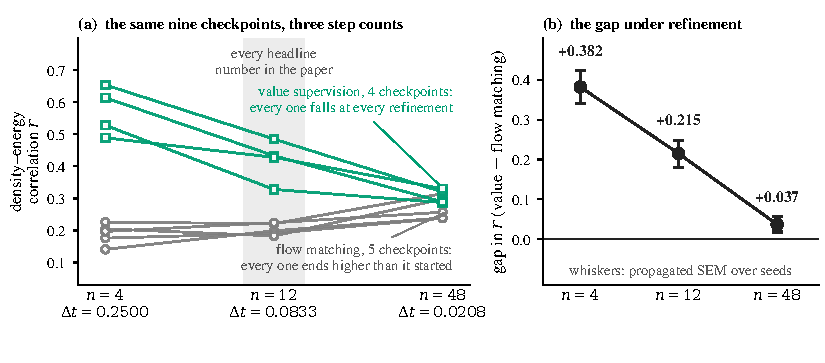
\includegraphics[width=\linewidth]{figures/out/figA_resolution.pdf}
\end{center}
\caption{\textbf{The paired resolution sweep.} The same nine checkpoints ---
five flow-matching controls (seeds $1$--$5$) and four value runs (seeds
$1$, $2$, $3$, $5$) --- re-scored at $n = 4$, $n = 12$ and $n = 48$ ODE steps on
identical parents, identical displacements and a pinned evaluation seed.
\textbf{(a)} Per checkpoint: all four value checkpoints fall at every
refinement, and all five flow-matching checkpoints end higher at $n = 48$ than
at $n = 4$, three of them monotonically. \textbf{(b)} The arm gap decays
$+0.382 \rightarrow +0.215 \rightarrow +0.037$. Each point is the difference of
the two arm means over independently trained seeds, five control and four
value, and each whisker is the propagated standard error over those seeds, a
descriptive SEM rather than a confidence interval. Every number reported
elsewhere in the paper is computed at $n = 12$. The value loss was itself
computed at $n = 4$, so one reading of the decay is that the ordering the term
teaches is expressed most strongly in the object the coarse estimator reports;
that is offered as a reading and not as a demonstrated mechanism. What the
analysis establishes is that the estimator is sensitive to solver resolution.
It does not distinguish model-dependent numerical error from an effect learned
under the four-step training estimator.}
\label{fig:resolution}
\end{figure}

% It must NOT go in the main text: the nine-page main text has no vertical slack
% and this figure is a diagnostic, not a result.
%
% Image produced by figures/figA_resolution.py, which also writes
% figures/out/figA_resolution_data.json recording every number drawn.
%
% PROVENANCE.  The per-checkpoint values are the authoritative re-scoring of the
% records under runs/eval_res/{a1_fm_only,a3_energy_only}[_s<N>]__ode{4,12,48};
% they are transcribed, not recomputed, per the standing instruction.  The
% generator recomputes every AGGREGATE (arm means, gaps, Welch t) from those
% per-checkpoint values and refuses to draw unless each reproduces the
% authoritative aggregate; it also checks the two directional counts the figure
% states before stating them.  The Welch t values stay inside that gate and
% inside figA_resolution_data.json: NO t value and NO significance label is
% rendered in the image or in the caption.  Panel (b) is descriptive -- the
% difference of arm means with the propagated SEM over seeds.
%
% Drawn at final size (5.5 x 2.42 in) with an explicit, non-tight bounding box;
% include with width=\linewidth, never \resizebox.
\begin{figure}[t]
\begin{center}
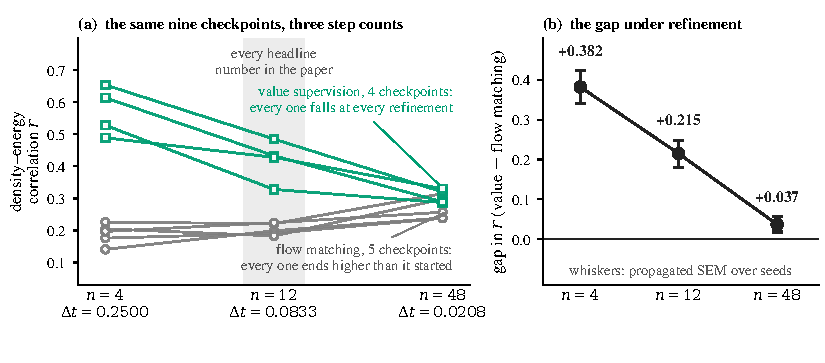
\includegraphics[width=\linewidth]{figures/out/figA_resolution.pdf}
\end{center}
\caption{\textbf{The paired resolution sweep.} The same nine checkpoints ---
five flow-matching controls (seeds $1$--$5$) and four value runs (seeds
$1$, $2$, $3$, $5$) --- re-scored at $n = 4$, $n = 12$ and $n = 48$ ODE steps on
identical parents, identical displacements and a pinned evaluation seed.
\textbf{(a)} Per checkpoint: all four value checkpoints fall at every
refinement, and all five flow-matching checkpoints end higher at $n = 48$ than
at $n = 4$, three of them monotonically. \textbf{(b)} The arm gap decays
$+0.382 \rightarrow +0.215 \rightarrow +0.037$. Each point is the difference of
the two arm means over independently trained seeds, five control and four
value, and each whisker is the propagated standard error over those seeds, a
descriptive SEM rather than a confidence interval. Every number reported
elsewhere in the paper is computed at $n = 12$. The value loss was itself
computed at $n = 4$, so one reading of the decay is that the ordering the term
teaches is expressed most strongly in the object the coarse estimator reports;
that is offered as a reading and not as a demonstrated mechanism. What the
analysis establishes is that the estimator is sensitive to solver resolution.
It does not distinguish model-dependent numerical error from an effect learned
under the four-step training estimator.}
\label{fig:resolution}
\end{figure}


\paragraph{What it settles, and what it does not.} Three observations, stated
descriptively. \emph{(a) The gap is present at the resolution we report.} At $n = 12$
the two arm means are $+0.418 \pm 0.033$ over four value seeds and $+0.204 \pm 0.008$
over five control seeds, for $\Delta r = +0.215$; the four value checkpoints span
$0.328$--$0.485$ and the five control checkpoints span $0.183$--$0.224$, so the two
observed seed ranges do not overlap. The same checkpoints scored under the paper's own
evaluation draw give $+0.182$ on the same 120-parent, geometry-dropped population
(\Cref{tab:scaleperm}, block 2: $0.397$ against $0.215$). The two agree in sign and in
size to within $0.033$, which is a consistency check and not an independent
replication: the checkpoints are one family, and what differs is the pinned evaluation
draw. \emph{(b) The magnitude of the observed gap decreases as the finite-step
estimator is refined.} It is $+0.382$ at $n = 4$, $+0.215$ at $n = 12$ and $+0.037$ at
$n = 48$. At $n = 48$ the two observed seed ranges do overlap: the value checkpoints
span $0.287$--$0.330$ and the control checkpoints $0.238$--$0.315$. Every headline
number in this paper is computed at $n = 12$. \emph{(c) The two arms move in opposite
directions under refinement.} The value arm falls from $+0.571$ to $+0.306$ while the
flow-matching arm rises from $+0.189$ to $+0.269$, and \Cref{tab:reschk} shows the split
holds checkpoint by checkpoint: all four value checkpoints fall at every refinement,
and all five control checkpoints end higher at $n = 48$ than at $n = 4$, three of them
monotonically.

One reading we offer --- as a reading, not as an established mechanism --- is that the
value loss was itself computed at $n = 4$, and so shaped the object the $n = 4$
estimator reports: the model would then have learned to order the density at the
resolution its training objective could see, and that ordering would weaken as the
estimate is refined. What this analysis establishes is estimator-resolution
sensitivity: it does not distinguish model-dependent numerical error from an effect
learned specifically under the four-step training estimator, and the observed
arm-dependent trends are consistent with either. Whichever the source, the effect size
is a property of the pair (model, step count) and not of the model alone, which is why
every number in this paper is quoted with the step count it was computed at, and why
the $n = 48$ row is reported here in full rather than summarised.

\paragraph{The second resolution family, and why it is supporting rather than
primary.} A second complete re-scoring at more than one step count exists in the run
store, on the checkpoints of the matched grid rather than on the earlier arms: cells A
and D of \Cref{app:p0cells} were re-scored at $n = 4$ and $n = 48$ under the same
geometry-dropped, 120-parent convention. It is listed here with its values and its
coverage rather than set aside without one, and \Cref{tab:resother} gives it in full.
Two properties keep it out of the primary comparison and neither is a matter of
preference. First it is \emph{incomplete in the step dimension}: it carries $n = 4$ and
$n = 48$ but no $n = 12$ row, so it cannot be read at the resolution every reported
number in this paper uses, and it supplies two points of a curve rather than three.
Second its value arm is drawn from a \emph{different seed set} from the matched design:
its six D checkpoints are the three matched-block seeds together with three of the
later independently launched seeds, which the reporting rules of \Cref{app:p0cells}
forbid merging into a matched-grid mean. It is also a different evaluation draw from
the family of \Cref{tab:respaired}, being scored on the grid's own parents and
displacements rather than on the earlier round's, so the two families' rows are not
byte-paired with one another even though each is internally paired across step counts.
We therefore classify it as \emph{supporting evidence for the numerical sensitivity of
the estimator}, not as a second matched primary comparison, and no contrast in this
paper is formed from it. What it adds is that the same two directions appear on an
independent set of checkpoints: between $n = 4$ and $n = 48$ the value-carrying cell
falls from $+0.614$ to $+0.314$ while the physics-free cell rises from $+0.161$ to
$+0.261$, and the difference of arm means falls from $+0.453$ to $+0.053$.

\begin{table}[h]
\caption{The second, supporting resolution family: cells A and D of the matched grid
(\Cref{app:p0cells}) re-scored at two step counts, 120 parents, data geometry dropped,
GFN2-xTB, evaluation seed pinned across step counts within this family. Entries are arm
means over checkpoints $\pm$ the standard error over checkpoints, with every
per-checkpoint value printed beside them. This family is \textbf{not} a matched primary
comparison and no contrast in this paper is formed from it: it carries no $n = 12$ row,
so it cannot be read at the resolution the paper reports, and its D arm mixes the three
matched-block seeds ($s2$, $s3$, $s5$) with three later independently launched seeds
($s6$, $s7$, $s9$), which the reporting rules of \Cref{app:p0cells} keep separate. It is
recorded as supporting evidence for the estimator's resolution sensitivity.
Recomputed for this table from the family's own per-record evaluation outputs by the
same per-group routine that produces \Cref{tab:reschk}.}
\label{tab:resother}
\begin{center}
\footnotesize
\setlength{\tabcolsep}{5pt}
\begin{tabular}{llcc}
\toprule
Cell & per-checkpoint $r$ & mean $\pm$ SEM & \\
\midrule
\multicolumn{4}{@{}l}{\emph{$n = 4$ (the training resolution)}} \\
D \texttt{energy} (6 ckpts) & $0.652$, $0.647$, $0.592$, $0.618$, $0.569$, $0.605$ & $+0.614 \pm 0.013$ & \\
A \texttt{fmonly} (5 ckpts) & $0.174$, $0.137$, $0.165$, $0.188$, $0.142$ & $+0.161 \pm 0.010$ & \\
 & & $\Delta r = +0.453$ & \\
\midrule
\multicolumn{4}{@{}l}{\emph{$n = 12$}} \\
\multicolumn{3}{@{}l}{\emph{not scored in this family}} & \\
\midrule
\multicolumn{4}{@{}l}{\emph{$n = 48$}} \\
D \texttt{energy} (6 ckpts) & $0.358$, $0.308$, $0.347$, $0.271$, $0.297$, $0.301$ & $+0.314 \pm 0.013$ & \\
A \texttt{fmonly} (5 ckpts) & $0.229$, $0.269$, $0.273$, $0.290$, $0.243$ & $+0.261 \pm 0.011$ & \\
 & & $\Delta r = +0.053$ & \\
\bottomrule
\end{tabular}
\end{center}
\end{table}

\paragraph{What would actually settle it.} There is no coupling defect to repair here:
the scheme integrates over the whole of $[0,1]$ and targets $\log q_\theta$ at $t = 1$
at every step count. What there is instead is bias --- first order in $\Delta t$ from
the Euler state integration against $O(\Delta t^2)$ from the quadrature --- and no step
count reported in this paper demonstrates a plateau, so we claim convergence for none
of these numbers. The missing measurements are the ordinary numerical ones: a
higher-order or adaptive integrator for the state, and more steps at both training and
evaluation time until the reported value stops moving. To those the opposite-direction
result of \Cref{tab:reschk} adds one more: an arm whose value term is computed at the
resolution the evaluation uses, which is the comparison that would separate the
solver's contribution from what the coarse objective taught. We have not run them, and
no result in this paper reflects them.

\subsection{Calibration diagnostics, per-seed values, and the teacher-evaluator agreement reference}
\label{app:scalediag}

This subsection gives the definitions behind the calibration endpoint, every
per-seed value behind every mean in \Cref{tab:primary} and \Cref{fig:calibration},
the sensitivity of those numbers to the two evaluation corrections, and how the
teacher-evaluator agreement reference is measured.

% ---------------------------------------------------------------------------
%  RELOCATED FROM THE MAIN TEXT BY THE 2026-08-19 COMPRESSION PASS.  This was
%  Table 1 of the pre-compression manuscript; the caption is unchanged apart
%  from cross-references that pointed at main-text floats.  Every number it
%  carries is also stated in the prose of Sec. 5.2 and Sec. 5.3.
% ---------------------------------------------------------------------------
\begin{table}[h]
\caption{\textbf{The primary endpoint}: 93 held-out parents disjoint from the value term's shard
pool, data geometry dropped, $8$ displaced geometries each, every energy a GFN2-xTB single point
from an evaluator independent of the eSEN training teacher. $r$ is the per-parent correlation between $\log q_\theta$, the clamped positional-flow density,
and $-E/kT$, averaged over parents then seeds ($\pm$ SEM over seeds);
$\mathrm{NRV}$ \eqref{eq:rm} is the median over parents per seed, then the mean over seeds, and is
anchored: \textbf{a constant log-density scores exactly $1$}. $kT_{\mathrm{eff}}$ ideally equals
the $1.0$~eV training target, and retrieval is against $12.5\%$ and $37.5\%$ at chance. The last row is
\emph{not a model} but the teacher's own energies through the identical pipeline, reported for $r$
and retrieval only; it is a reference for what exact reproduction of the teacher would score on
this ensemble, not an attainable maximum, and its calibration diagnostics are derived in
\Cref{fig:calibration}. $^{\dagger}$The scrambled row is a defective control, one of its two shards
having been left unscrambled and its third seed not configuration-matched, and is superseded by cell C of
\Cref{fig:grid}; a fourth seed of that arm completed but lost its evaluation to a launcher fault
and is recovered in \Cref{app:cells}, where it lowers the arm further. Launch record for the three
trained arms (\Cref{app:cells}): flow matching $5$ prepared / $5$ completed / $0$ diverged, all five
scored here, the fifth having been a finite completed checkpoint that was scored under this
protocol only later (\Cref{app:cells}); value $5$ / $4$ / $1$, all four scored; scrambled
$7$ / $4$ / $3$, three of them scored. Value entries are therefore conditional on completion
(\Cref{sec:method}).}
\label{tab:primary}
\begin{center}
\small
\setlength{\tabcolsep}{5pt}
\begin{tabular}{lccccc}
\toprule
Arm & seeds & $r$ $\uparrow$ & $\mathrm{NRV}$ $\downarrow$ & $kT_{\mathrm{eff}}$ (eV) & top-1 / top-3 $\uparrow$ \\
\midrule
Flow matching only          & 5 & $0.200 \pm 0.018$ & $1.402$ & $8.02$ & $20.2\%$ / $49.5\%$ \\
\textbf{Value (ours)}       & 4 & $\mathbf{0.369 \pm 0.023}$ & $2.144$ & $2.34$ & $\mathbf{29.6\%}$ / $\mathbf{62.4\%}$ \\
Energies scrambled$^{\dagger}$ & 3 & $0.226 \pm 0.020$ & n/a & n/a & n/a \\
\midrule
\emph{Teacher-evaluator agreement} & n/a & $0.927$ & n/a & n/a & $87.1\%$ / $98.9\%$ \\
\bottomrule
\end{tabular}
\end{center}
\end{table}

\paragraph{Definitions, and the two identities that make them readable.} For a
parent with $K$ geometries, $\mathrm{NRV}$ is \eqref{eq:rm}, the slope is the
ordinary least-squares slope of $\log q_\theta$ on $-E/kT$, the scale ratio is
$\mathrm{sd}_k[\log q_\theta]/\mathrm{sd}_k[E/kT]$, and
$kT_{\mathrm{eff}} = kT/\mathrm{slope} = -\Var_k(E)/\Cov_k(\log q_\theta, E)$,
which is invariant to the $kT$ used to form it and is therefore a statement about
the model and not about our choice of scale. Writing
$a = \Var(\log q_\theta)/\Var(E)$ and $b = \Cov(\log q_\theta,E)/\Var(E)$, rescaling
$\log q_\theta \mapsto s\log q_\theta$ traces the parabola
$\mathrm{NRV}(s) = a\,s^2 + 2b\,s + 1$, minimised at $s^{*} = -b/a$ with value
$1-r^2$, which is the $\mathrm{NRV}_{\min}$ of \eqref{eq:rm}: no rescaling, and
equivalently no single temperature, can bring the normalised residual below that
floor. (We write the free parameter as the dimensionless rescaling $s$ rather than
as a temperature; the temperature reading $kT' = kT/s$ is a corollary.) Finally
$\mathrm{slope} = r \times (\text{scale ratio})$ splits the slope into direction and
magnitude, and by \eqref{eq:app-nrvtau} $\mathrm{NRV}$ is exactly the $\tau^2$ of
\Cref{prop:surrogate}. That identity holds within a single group under a single
potential; $\mathrm{NRV}$ is therefore the normalised evaluation analogue of the same
Boltzmann-residual form the training objective uses, and the two share that residual
structure while being evaluated with different potentials, populations and integrator
step counts.

\paragraph{Aggregation, and why we quote medians.} $\mathrm{NRV}$ is heavy-tailed
across parents: groups whose $\Var_k[E]$ is near zero divide by almost nothing, and
one flow-matching seed has a \emph{mean} $\mathrm{NRV}$ in the thousands driven by a
single group. We therefore report the median over parents for each seed and then the
mean over seeds, while $r$ is a mean over parents and then over seeds; the analysis
script additionally emits a $10\%$ trimmed mean and bootstrap intervals. Paired
per-parent comparisons are reported as the median paired shift in the per-parent,
seed-median values over the same parents, together with the count of parents that move
in each direction; the signed-rank statistics computed alongside them are collected in
\Cref{tab:inferential} and are not used anywhere in the argument.

\begin{table}[h]
\caption{Every seed behind \Cref{tab:primary} and \Cref{fig:calibration}, on the
primary endpoint (93 parents disjoint from the value term's shard pool, data geometry
dropped, GFN2-xTB energies, $n = 12$). $r$ and the scale ratio are means over parents
within a seed; $\mathrm{NRV}$, $\mathrm{NRV}_{\min}$, the slope and
$kT_{\mathrm{eff}}$ are medians over parents within a seed. Arm rows are the mean over
seeds with the standard error over seeds. Recomputed for this table from the per-seed
blocks of the calibration analysis, restricted to the 93 disjoint parents; the $r$ and
$\mathrm{NRV}$ columns reproduce \Cref{tab:primary} exactly. Seed numbers are
within-arm labels listed in run order and do not pair across arms: the arms were
trained independently and nothing here is a paired comparison at the seed level.
$^{\ast}$Seed 5 of the flow-matching arm is the later-scored control seed of
\Cref{app:cells}: a checkpoint that completed the full budget with finite weights but
carried no score under this protocol until it was scored under it, on the identical
parents, displacements and estimator settings.}
\label{tab:scaleseeds}
\begin{center}
\footnotesize
\setlength{\tabcolsep}{4pt}
\begin{tabular}{llcccccc}
\toprule
Arm & seed & $r$ & $\mathrm{NRV}$ & $\mathrm{NRV}_{\min}$ & slope & scale ratio & $kT_{\mathrm{eff}}$ (eV) \\
\midrule
Flow matching only
 & 1 & $0.222$ & $1.393$ & $0.810$ & $0.142$ & $0.906$ & $7.04$ \\
 & 2 & $0.194$ & $1.342$ & $0.848$ & $0.094$ & $0.808$ & $10.63$ \\
 & 3 & $0.249$ & $1.337$ & $0.816$ & $0.162$ & $0.854$ & $6.17$ \\
 & 4 & $0.142$ & $1.548$ & $0.847$ & $0.110$ & $0.768$ & $9.06$ \\
 & 5$^{\ast}$ & $0.192$ & $1.388$ & $0.803$ & $0.139$ & $0.810$ & $7.18$ \\
 & \emph{mean} & $0.200$ & $1.402$ & $0.825$ & $0.130$ & $0.829$ & $8.02$ \\
 & \emph{s.e.m.} & $0.018$ & $0.038$ & $0.009$ & $0.012$ & $0.024$ & $0.81$ \\
\midrule
\textbf{Value (ours)}
 & 1 & $0.316$ & $2.955$ & $0.782$ & $0.427$ & $1.763$ & $2.34$ \\
 & 2 & $0.378$ & $2.738$ & $0.753$ & $0.538$ & $1.609$ & $1.86$ \\
 & 3 & $0.426$ & $1.547$ & $0.714$ & $0.513$ & $1.210$ & $1.95$ \\
 & 4 & $0.358$ & $1.337$ & $0.737$ & $0.313$ & $0.994$ & $3.19$ \\
 & \emph{mean} & $0.369$ & $2.144$ & $0.747$ & $0.448$ & $1.394$ & $2.34$ \\
 & \emph{s.e.m.} & $0.023$ & $0.410$ & $0.014$ & $0.051$ & $0.177$ & $0.30$ \\
\midrule
Energies scrambled
 & 1 & $0.226$ & $1.727$ & $0.791$ & $0.244$ & $1.086$ & $4.09$ \\
 & 2 & $0.192$ & $1.757$ & $0.829$ & $0.176$ & $1.001$ & $5.70$ \\
 & 3 & $0.260$ & $1.754$ & $0.792$ & $0.228$ & $1.076$ & $4.39$ \\
 & \emph{mean} & $0.226$ & $1.746$ & $0.804$ & $0.216$ & $1.054$ & $4.73$ \\
 & \emph{s.e.m.} & $0.020$ & $0.010$ & $0.013$ & $0.021$ & $0.027$ & $0.49$ \\
\bottomrule
\end{tabular}
\end{center}
\end{table}

\paragraph{Sensitivity to the two evaluation corrections.} The primary endpoint
applies two corrections at once --- restrict to the 93 parents outside the shard pool,
and drop the high-leverage data geometry --- and both \emph{reduce} the contrast we
report. \Cref{tab:scaleperm} gives the same diagnostics on the three other
populations that the same records support, so that the sensitivity of every number to
those two choices is visible. All four blocks come from one round, one set of seeds
and one re-scored per-record source, and differ only in which parents and which
geometries enter each group; none of them may be compared with the earlier, smaller
round of \Cref{app:cells}. The ordering endpoint is highest and the calibration
endpoint most flattering on the permissive population, which is why the restrictive
one is primary.

\begin{table}[h]
\caption{Sensitivity of every calibration diagnostic to the two evaluation
corrections. Block 1 is the primary endpoint and is identical to the arm rows of
\Cref{tab:scaleseeds}; the other three blocks relax one or both corrections. Entries
are means over seeds $\pm$ the standard error over seeds, with the same
median-over-parents convention. Recomputed for this table from the per-seed blocks of
the calibration analysis. A \emph{constant} log-density scores $\mathrm{NRV} = 1$
exactly, so no arm in any block is calibrated.}
\label{tab:scaleperm}
\begin{center}
\scriptsize
\setlength{\tabcolsep}{2.5pt}
\begin{tabular}{lccccccc}
\toprule
Arm & seeds & $\mathrm{NRV}$ & $\mathrm{NRV}_{\min}$ & slope & scale ratio & $kT_{\mathrm{eff}}$ (eV) & $r$ \\
\midrule
\multicolumn{8}{l}{\emph{Block 1 --- 93 disjoint parents, data geometry dropped (the primary endpoint)}} \\
Flow matching only  & 5 & $1.402 \pm 0.038$ & $0.825 \pm 0.009$ & $0.130 \pm 0.012$ & $0.829 \pm 0.024$ & $8.02 \pm 0.81$ & $0.200 \pm 0.018$ \\
Energies scrambled  & 3 & $1.746 \pm 0.010$ & $0.804 \pm 0.013$ & $0.216 \pm 0.021$ & $1.054 \pm 0.027$ & $4.73 \pm 0.49$ & $0.226 \pm 0.020$ \\
Value (ours)        & 4 & $2.144 \pm 0.410$ & $0.747 \pm 0.014$ & $0.448 \pm 0.051$ & $1.394 \pm 0.177$ & $2.34 \pm 0.30$ & $0.369 \pm 0.023$ \\
\midrule
\multicolumn{8}{l}{\emph{Block 2 --- all 120 parents, data geometry dropped}} \\
Flow matching only  & 5 & $1.382 \pm 0.029$ & $0.827 \pm 0.009$ & $0.148 \pm 0.010$ & $0.833 \pm 0.019$ & $6.88 \pm 0.46$ & $0.215 \pm 0.015$ \\
Energies scrambled  & 3 & $1.691 \pm 0.015$ & $0.797 \pm 0.012$ & $0.236 \pm 0.027$ & $1.084 \pm 0.034$ & $4.35 \pm 0.51$ & $0.254 \pm 0.022$ \\
Value (ours)        & 4 & $2.024 \pm 0.377$ & $0.736 \pm 0.015$ & $0.548 \pm 0.053$ & $1.420 \pm 0.183$ & $1.88 \pm 0.19$ & $0.397 \pm 0.022$ \\
\midrule
\multicolumn{8}{l}{\emph{Block 3 --- 93 disjoint parents, data geometry retained}} \\
Flow matching only  & 5 & $1.303 \pm 0.029$ & $0.849 \pm 0.004$ & $0.028 \pm 0.008$ & $0.514 \pm 0.005$ & $52.2 \pm 15.9$ & $0.060 \pm 0.016$ \\
Energies scrambled  & 3 & $1.061 \pm 0.051$ & $0.782 \pm 0.020$ & $0.232 \pm 0.023$ & $0.723 \pm 0.023$ & $4.40 \pm 0.41$ & $0.325 \pm 0.037$ \\
Value (ours)        & 4 & $1.189 \pm 0.173$ & $0.711 \pm 0.030$ & $0.451 \pm 0.046$ & $1.049 \pm 0.144$ & $2.30 \pm 0.28$ & $0.420 \pm 0.034$ \\
\midrule
\multicolumn{8}{l}{\emph{Block 4 --- all 120 parents, data geometry retained (the fully permissive metric)}} \\
Flow matching only  & 5 & $1.282 \pm 0.027$ & $0.845 \pm 0.005$ & $0.059 \pm 0.007$ & $0.556 \pm 0.009$ & $17.8 \pm 2.1$ & $0.088 \pm 0.014$ \\
Energies scrambled  & 3 & $1.062 \pm 0.045$ & $0.777 \pm 0.021$ & $0.259 \pm 0.033$ & $0.736 \pm 0.029$ & $3.97 \pm 0.46$ & $0.341 \pm 0.039$ \\
Value (ours)        & 4 & $1.211 \pm 0.181$ & $0.708 \pm 0.030$ & $0.491 \pm 0.045$ & $1.093 \pm 0.159$ & $2.09 \pm 0.21$ & $0.434 \pm 0.032$ \\
\bottomrule
\end{tabular}
\end{center}
\end{table}

\paragraph{The paired per-parent comparisons in full.} The seed-level tests above
have four and five units of replication, which is the unit of replication for a claim
about a training method. The parent-level tests below have 93 units \emph{within} those
same nine models: they show how the shift is distributed across the evaluation set, and
they are not additional training replications. All are paired per-parent differences of
seed-median values over the same 93 parents with the data geometry dropped, value arm
minus flow-matching control, recomputed for this pass from the per-seed calibration
blocks; we quote the median paired shift, and the value term improves on every
ordering-flavoured diagnostic: per-group correlation (median $\Delta = +0.182$),
regression slope ($+0.346$), scale ratio ($+0.500$) and the temperature-optimal bound
$1-r^2$ ($-0.055$). On $\mathrm{NRV}$ it is \emph{worse}, by $+0.476$. The value term
raises the per-parent correlation on $67$ of the $93$ parents. Parent-level paired
analyses therefore show the shift distributed broadly across the
evaluation set, and the two endpoints disagree in sign there as well as at seed level, which is the finding \Cref{sec:scale} reports and limitation (i)
records. The fraction of parents clearing the constant-density bar $\mathrm{NRV} < 1$
is $0.258 \pm 0.044$ under the value term and $0.286 \pm 0.025$ under the control.

\paragraph{The retrieval read-out.} Retrieval is computed from the same per-record
source: for each parent the 8 displaced geometries are ranked by $\log q_\theta$ and
we ask whether the top one, or the top three, contain the geometry GFN2-xTB scores
lowest. Chance is $1/8 = 12.5\%$ and $3/8 = 37.5\%$. The read-out is invariant to
both the per-group additive constant and any positive rescaling of $\log q_\theta$,
so it survives the calibration failure of \Cref{sec:scale} intact; it was added after
the evaluation was designed and is not a pre-registered endpoint.

\begin{table}[h]
\caption{Retrieval, per seed, on the primary endpoint. Each entry is the fraction of
the 93 parents whose lowest-energy displaced geometry is ranked first (top-1) or in
the top three (top-3) by $\log q_\theta$. Chance is $12.5\%$ and $37.5\%$. The
teacher row substitutes $-E_{\mathrm{eSEN}}/kT$ for $\log q_\theta$ on the identical
geometries and is not a model. Seed numbers are within-arm labels and do not pair
across arms; seed 5 of the flow-matching arm is the later-scored control seed of
\Cref{app:cells}, and the value arm has four seeds, so its seed-5 cells are empty.}
\label{tab:retrieval}
\begin{center}
\footnotesize
\begin{tabular}{lcccccc}
\toprule
Arm & seed 1 & seed 2 & seed 3 & seed 4 & seed 5 & mean \\
\midrule
Flow matching only, top-1 & $23.7\%$ & $19.4\%$ & $20.4\%$ & $15.1\%$ & $22.6\%$ & $20.2\%$ \\
\textbf{Value (ours)}, top-1 & $26.9\%$ & $33.3\%$ & $28.0\%$ & $30.1\%$ & --- & $\mathbf{29.6\%}$ \\
\midrule
Flow matching only, top-3 & $49.5\%$ & $49.5\%$ & $50.5\%$ & $47.3\%$ & $50.5\%$ & $49.5\%$ \\
\textbf{Value (ours)}, top-3 & $64.5\%$ & $65.6\%$ & $62.4\%$ & $57.0\%$ & --- & $\mathbf{62.4\%}$ \\
\midrule
\emph{Teacher} (not a model) & --- & --- & --- & --- & --- & $87.1\%$ / $98.9\%$ \\
\bottomrule
\end{tabular}
\end{center}
\end{table}

\paragraph{The teacher-evaluator agreement reference, and why it must be re-measured on any
other ensemble.} The reference is measured, not assumed: the identical geometries are scored
with the eSEN teacher \citep{esen}, $-E_{\mathrm{eSEN}}/kT$ is substituted for
$\log q_\theta$, and the result is pushed through the same per-group code. One
reference run serves every arm of the round, because their geometries are
byte-identical. On the 93 primary parents with the data geometry dropped it gives
$r = 0.927$; the same construction over all 120 parents gives $0.933$, quoted here
for context only and never mixed with a model number computed on a different
population. The value arm's $0.369$ is therefore about $40\%$ of the teacher-evaluator agreement reference
on this ensemble in absolute terms, and closes $23.3\%$ of the gap to it. A model
could in principle align with GFN2-xTB better than the teacher does, so this is a
reference and not an attainable maximum.

The reference is high because the ensemble is wide, which is a property of the ensemble
rather than of the method. On the 93 primary parents with the data geometry dropped the
within-group spread of $E_{\mathrm{GFN2-xTB}}$ is $14.3$~eV on average (median
$10.7$~eV, maximum $50.2$~eV), while the teacher--evaluator disagreement on
\emph{relative} energies inside a group is $4.15$~eV mean absolute (median $2.19$~eV).
Two potentials that disagree by a few eV will still rank a fifteen-eV window
consistently while saying much less about agreement inside a thermally accessible one,
so a narrower perturbation ensemble has a materially lower reference. We therefore state
the rule rather than a projection: every new ensemble needs its teacher-evaluator agreement
reference measured directly, and no correlation computed on one ensemble may be read as
a fraction of a reference measured on another.

\paragraph{The same calibration diagnostics scored with the training teacher.} A
calibration failure measured with an independent potential invites one specific
objection: that what is being measured is disagreement between the evaluator and the
teacher the model was trained against, rather than a property of the learned density.
The records answer it directly. The eSEN teacher's energies for all $1080$ held-out
geometries are on file, so the calibration diagnostics can be recomputed on the
\emph{same} 93 parents, the same displacements and the same model log-densities, with
the scorer as the only thing that changes. To keep the two columns produced by one code
path, each arm's per-record file was copied with its energy column replaced by the
teacher energy for the matching (parent, displacement) pair, and the paper's own
calibration analysis was then run on the copies with the reference geometry dropped and
$kT = 1.0$~eV, exactly as for the reported column; the 93-parent restriction and the
median-over-parents-then-mean-over-seeds aggregation are the same routines that produce
\Cref{tab:scaleseeds}. Run this way the pipeline returns the reported GFN2-xTB column
unchanged to the last printed digit --- $r = 0.200 / 0.369$, $\mathrm{NRV} = 1.402 /
2.144$, $\mathrm{NRV}_{\min} = 0.825 / 0.747$, slope $= 0.130 / 0.448$ and
$kT_{\mathrm{eff}} = 8.02 / 2.34$~eV --- which is what licenses reading the second
column beside it. \textbf{No GFN2-xTB number in this paper changes.}

\begin{table}[h]
\caption{The calibration diagnostics of \Cref{tab:scaleseeds} recomputed with the
training teacher in place of the independent evaluator. Same 93 primary parents, same
displaced geometries, same model log-densities at $n = 12$, same $kT = 1.0$~eV, same
aggregation (median over parents within a seed, then mean over seeds $\pm$ the standard
error over seeds; $r$ and $\mathrm{NRV}_{\min}$ are means over parents). Only the energy
column differs. The GFN2-xTB block is the reported primary endpoint and is reproduced
here by the identical code path. $kT_{\mathrm{eff}}$ ideally equals the $1.0$~eV
training target; a constant log-density scores $\mathrm{NRV} = 1$ exactly, so no arm
under either scorer clears that bar.}
\label{tab:esencalib}
\begin{center}
\footnotesize
\setlength{\tabcolsep}{2.5pt}
\begin{tabular}{lcccccc}
\toprule
Arm & seeds & $r$ $\uparrow$ & $\mathrm{NRV}$ $\downarrow$ & $\mathrm{NRV}_{\min}$ $\downarrow$ & slope & $kT_{\mathrm{eff}}$ (eV) \\
\midrule
\multicolumn{7}{l}{\emph{Scored with GFN2-xTB --- the independent evaluator (the reported primary endpoint)}} \\
Flow matching only & 5 & $0.200 \pm 0.018$ & $1.402 \pm 0.038$ & $0.825 \pm 0.009$ & $0.130 \pm 0.012$ & $8.02 \pm 0.81$ \\
Value (ours)       & 4 & $0.369 \pm 0.023$ & $2.144 \pm 0.410$ & $0.747 \pm 0.014$ & $0.448 \pm 0.051$ & $2.34 \pm 0.30$ \\
\midrule
\multicolumn{7}{l}{\emph{Scored with eSEN --- the potential the value term was trained against}} \\
Flow matching only & 5 & $0.202 \pm 0.018$ & $1.676 \pm 0.025$ & $0.821 \pm 0.009$ & $0.189 \pm 0.017$ & $5.52 \pm 0.67$ \\
Value (ours)       & 4 & $0.399 \pm 0.027$ & $2.821 \pm 0.576$ & $0.716 \pm 0.018$ & $0.718 \pm 0.043$ & $1.41 \pm 0.09$ \\
\bottomrule
\end{tabular}
\end{center}
\end{table}

Three things follow. First, the raw normalised residual variance worsens against the
training teacher as well, and by more than against the independent evaluator: $1.676
\to 2.821$ under eSEN against $1.402 \to 2.144$ under GFN2-xTB. The failure to
calibrate is therefore not an artefact of transferring from the teacher to a different
potential; it is present against the very potential the model was trained against, and
the ordering-without-calibration reading of \Cref{sec:scale} holds under both scorers.
Second, the two endpoints separate more sharply against the teacher, not less: the
slope rises from $0.448$ to $0.718$ and $kT_{\mathrm{eff}}$ moves from $2.34$~eV to
$1.41$~eV against the $1.0$~eV numerical target, while $\mathrm{NRV}$ moves the other
way. That is the mechanism \Cref{sec:scale} states --- the direction of the density's
response and its optimal rescaling improve while the residual that no single rescaling
can remove grows --- and seeing it more clearly under the teacher corroborates it.
Third, the ordering endpoint is close to scorer-independent for the control ($0.200$
against $0.202$) and somewhat higher for the value arm ($0.369$ against $0.399$), so
the independent evaluator is if anything the more conservative choice for the
comparison this paper reports, and it remains the primary one for the reason given in
\Cref{app:eval}: it was not used to train the model.

\subsection{Perturbation families}
\label{app:perturb}

The reported groups are isotropic Gaussian displacements, which carry a confound that
this subsection quantifies and partly removes.

\paragraph{What every reported number uses, and the confound it carries.} All reported
evaluations use $x^{(k)} = x^{*} + \sigma\varepsilon$ with
$\varepsilon \sim \mathcal{N}(0,I)$ per coordinate and $\sigma = 0.15$~\AA{}, plus the
unperturbed data geometry; the training shards have the same character, with $K = 5$
geometries per parent at $\sigma \in \{0.03,0.06,0.10,0.20,0.40\}$~\AA{}. Because
$\lVert\varepsilon\rVert$ concentrates only as $O(1/\sqrt{3N})$, the members of a group
sit at \emph{different} distances from the data geometry: the mean root-mean-square
deviation is $\sigma\sqrt{3} \approx 0.25$~\AA{} and the within-group coefficient of
variation of that RMSD is $8.1\%$. Both $\log q_\theta$ and $E$ fall off with that
distance, so a model that had learned nothing beyond ``further from the data, lower
density'' would score a positive per-group correlation carrying no energy information
at all. That is why the confound has to be broken by construction rather than adjusted
for: the nuisance variable is held exactly constant in the fixed-RMSD family below, so
a residual contrast there cannot be a distance effect.

\paragraph{The generators, and which were evaluated.} Four perturbation generators are
implemented in pure array code --- \texttt{fixed\_rmsd}, \texttt{torsion},
\texttt{bond\_angle} and \texttt{normal\_mode} --- of which only \texttt{fixed\_rmsd}
and \texttt{normal\_mode} were used in any evaluation reported in this paper, and no
result for the other two appears anywhere. \texttt{fixed\_rmsd} draws a random
direction, projects out the six rigid-body modes, Kabsch-aligns the displaced geometry
to the reference and rescales the displacement by scalar bisection until the aligned
RMSD equals the requested value; a unit test over a set of molecules finds the realised
RMSD reproducing its target with standard deviation $1.3\times10^{-16}$~\AA{}, against
the $8.1\%$ coefficient of variation of the Gaussian family it replaces. The test
covers that the shell is exactly a shell; it does not establish, and we do not claim,
that a shell is a physically preferable ensemble. \texttt{normal\_mode} displaces along
a thermal-like combination of low-frequency modes from an anisotropic network model.

\paragraph{Status of the controlled evaluations.} On fixed-RMSD shells, with four seeds
per arm, the value arm reaches $+0.305$ against the flow-matching control's $+0.182$,
a difference of $\Delta r = +0.124$: the effect survives holding the geometry
distance exactly constant, at a reduced magnitude. On normal-mode displacements, with
five seeds per arm, the difference is $\Delta r = +0.185$, with a seed spread wide
enough that the two arms' observed ranges are not separated; it is reported as
supporting context only. The
torsional and bond-angle families, and the partial correlation
$r(\log q_\theta, -E \mid \mathrm{RMSD})$ that would quantify the residual radial
component inside the Gaussian family itself, have not been run, so the confound is
bounded rather than excluded (limitation (v)). One caveat travels with all of these:
by the reference argument of \Cref{app:scalediag}, a narrower perturbation ensemble
lowers the measurable teacher-evaluator agreement reference, so each controlled family would need
its own directly measured reference before its correlations were read as a fraction of
one. The two contrasts above are internally paired comparisons and nothing more.

\subsection{The matched six-cell grid}
\label{app:p0cells}

The grid is the experiment that isolates what the energy term contributes, among the runs
that completed. Six cells at five seeds each
are matched in every respect except the physics block, so that the differences between
columns are attributable to the physics block and to seed noise and to nothing else in
the pipeline.

\paragraph{Configuration.} Thirty training runs share: batch size 8 with two
accumulation steps, $30\,000$ optimiser steps, $\lambda_E = 3\times10^{-5}$ where
active, $\lambda_1 = 0.1$ where active, $\lambda_3 = 0$, parents per value step
$M = 8$, value-loss cap $1500$, the value term every fourth step on parents of at most
50 atoms, $n = 4$ integration steps and 2 Hutchinson probes, \emph{no} on-policy
distillation in any cell, and perturbation shards built from the \emph{training} split
only, so that no cell reads energies for a molecule the evaluation will see. All 30
runs warm-start from one common checkpoint at the end of epoch 0, so seed variation is
variation in the physics-carrying phase of training and not in the flow-matching
pre-phase. \Cref{tab:p0cells} gives what differs, together with the complete launch
record.

\begin{table}[h]
\caption{The matched grid: configuration and launch record. All six cells share every
hyperparameter listed in the text above; the table gives only what differs. ``Shard''
names the perturbation file the value term reads, all three built from the training
split of the same $30\,000$ parents and differing only in the energy column. The three
status columns are the launch record of the \emph{matched five-seed design} --- every seed
launched into it is counted and a diverged seed stays in the denominator --- and are themselves
a result, discussed below and in \Cref{app:stability}. Fourteen further runs of the same design
were launched afterwards and are reported separately below rather than folded into these
counts. Reading a cell by its
completions alone would condition on completion, which is not independent of the cell;
per-cell and per-seed results are \Cref{tab:p0seeds} and the two tables must be read
together.}
\label{tab:p0cells}
\begin{center}
\footnotesize
\setlength{\tabcolsep}{3pt}
\begin{tabular}{@{}l c c >{\raggedright\arraybackslash}p{0.86in} >{\raggedright\arraybackslash}p{1.30in} ccc@{}}
\toprule
Cell & $\lambda_1$ & $\lambda_E$ & Shard energies & What it isolates
  & \multicolumn{3}{c}{seeds} \\
\cmidrule(l){6-8}
 & & & & & launch & compl. & diverged \\
\midrule
A \texttt{fmonly}  & $0$   & $0$
  & \emph{no shard read}
  & baseline: flow matching alone
  & 5 & 5 & 0 \\
B \texttt{flat}    & $0$   & $3\times10^{-5}$
  & \emph{identically zero}
  & loss degenerates to $\Var_k[\log q_\theta]$: density regulariser, no energy label
  & 5 & 4 & 1 \\
C \texttt{scram}   & $0$   & $3\times10^{-5}$
  & permuted \emph{within} parent
  & $y$-randomisation: same multiset and spread, pairing destroyed
  & 5 & 5 & 0 \\
D \texttt{energy}  & $0$   & $3\times10^{-5}$
  & true teacher
  & the main effect
  & 5 & 3 & 2 \\
E \texttt{force}   & $0.1$ & $0$
  & \emph{no shard read}
  & gradient term, no distillation confound
  & 5 & 5 & 0 \\
F \texttt{both}    & $0.1$ & $3\times10^{-5}$
  & true teacher
  & gradient $+$ value
  & 5 & 2 & 3 \\
\midrule
\multicolumn{5}{@{}l}{\emph{total, cells without the value term} (A, E)}
  & \textbf{10} & \textbf{10} & \textbf{0} \\
\multicolumn{5}{@{}l}{\emph{total, cells with the value term} (B, C, D, F)}
  & \textbf{20} & \textbf{14} & \textbf{6} \\
\bottomrule
\end{tabular}
\end{center}
\end{table}

\paragraph{Results, per seed.} \Cref{tab:p0seeds} gives every completed evaluation of
the grid. Each entry is one training run, scored by the protocol of \Cref{app:eval} ---
120 held-out parents, one data geometry plus 8 Gaussian displacements at
$\sigma = 0.15$~\AA{} per parent, the data geometry \emph{dropped} before the per-group
Pearson correlation is formed, GFN2-xTB as the independent scorer, and $n = 12$
integration steps with 2 Hutchinson probes --- and the cell entry is the unweighted
mean over that cell's completed seeds with the standard error over seeds.

\begin{table}[h]
\caption{The matched grid, per seed and per cell. Mean per-group Pearson $r$ between
$\log q_\theta$ and $-E_{\mathrm{GFN2\text{-}xTB}}/kT$, 120 parents, \textbf{data
geometry excluded}, evaluated at $n = 12$. Every cell shares backbone, budget,
optimiser, warm start, evaluation protocol and training-split-only perturbation shards;
only $\lambda_1$, $\lambda_E$ and the shard's energy column differ. The seed counts here
are \emph{completions}: the launched/completed/diverged record is \Cref{tab:p0cells} and
must be read with this table, since completion is not independent of the cell
(limitation (viii)). The means of cells B, D and F are conditional on completion.}
\label{tab:p0seeds}
\begin{center}
\footnotesize
\setlength{\tabcolsep}{3.5pt}
\begin{tabular}{@{}l c c >{\raggedright\arraybackslash}p{1.12in} >{\raggedright\arraybackslash}p{1.74in} c@{}}
\toprule
Cell & $\lambda_1$ & $\lambda_E$ & Energy signal & per-seed $r$ & mean $\pm$ SEM \\
\midrule
A \texttt{fmonly}  & $0$   & $0$      & none (no shard)
  & $0.234$, $0.200$, $0.232$, $0.221$, $0.197$ & $+0.217 \pm 0.008$ \\
B \texttt{flat}    & $0$   & $3\times10^{-5}$ & all energies zero
  & $0.233$, $0.125$, $0.147$, $0.243$          & $+0.187 \pm 0.030$ \\
C \texttt{scram}   & $0$   & $3\times10^{-5}$ & scrambled within parent
  & $0.232$, $0.224$, $0.168$, $0.125$, $0.174$ & $+0.185 \pm 0.020$ \\
D \texttt{energy}  & $0$   & $3\times10^{-5}$ & true teacher
  & $0.452$, $0.398$, $0.412$                   & $\mathbf{+0.421 \pm 0.016}$ \\
E \texttt{force}   & $0.1$ & $0$      & none (no shard)
  & $0.105$, $0.130$, $0.044$, $0.086$, $0.058$ & $+0.085 \pm 0.016$ \\
F \texttt{both}    & $0.1$ & $3\times10^{-5}$ & true teacher
  & $0.179$, $0.210$                            & $+0.194 \pm 0.016$ \\
\bottomrule
\end{tabular}
\end{center}
\end{table}

\paragraph{The six contrasts the grid was built to run.} Each is the difference
$\Delta r$ between the seed means of two cells of \Cref{tab:p0seeds}, quoted with the
completed-seed counts behind it; the question each answers was fixed when the grid was
designed and is the reason that cell exists. Per-seed values for every cell are in
\Cref{tab:p0seeds} and every one of them is drawn in \Cref{fig:grid}.
\emph{(1) Does the value term work at all?} D versus A: $\Delta r = +0.204$
(3 vs 5 seeds) --- yes; every completed D seed ($0.398$--$0.452$) lies above every
completed A seed ($0.197$--$0.234$).
\emph{(2) Does it need the energy \emph{information}, or only the energy \emph{values}?}
D versus C, the $y$-randomisation control that keeps each parent's energy multiset and
within-parent spread and destroys only the geometry-to-energy pairing:
$\Delta r = +0.236$ (3 vs 5) --- it needs the pairing, and again the two observed seed
ranges do not overlap ($0.125$--$0.232$ for C).
\emph{(3) Is it more than a density regulariser?} D versus B, where the shard's energy
column is identically zero so the loss is exactly $\Var_k[\log q_\theta]$:
$\Delta r = +0.234$ (3 vs 4) --- yes, with B spanning $0.125$--$0.243$, again below
every D seed.
\emph{(4) What does the regulariser contribute on its own?} B versus A:
$\Delta r = -0.030$ (4 vs 5) --- \textbf{nothing measurable}: the point estimate is
negative and the two arms' seed ranges overlap almost completely.
\emph{(5) Does the gradient term work with the distillation confound removed?} E versus
A: $\Delta r = -0.132$ (5 vs 5) --- it is below the physics-free baseline, with every
E seed ($0.044$--$0.130$) below every A seed.
\emph{(6) Does the gradient term help on top of the value term?} F versus D:
$\Delta r = -0.227$ (2 vs 3) --- it does not; both F seeds lie below both the D range
and the A range.
Two cautions travel with all six. Every one of them rests on two to five completed
seeds per cell, so the separations above are statements about the observed seed
ranges of small samples and not asymptotic inferences; the arm means and their
standard errors are in \Cref{tab:p0seeds}. And contrasts (1)--(3) and (6) involve
cells D or F, whose means are over survivors. The three cells that completed at $5/5$,
$5/5$ and $4/5$ --- A, E and the zero-energy B --- are the ones entering contrasts (4)
and (5), the two negative or null results, which are therefore the least exposed to
selection.

\paragraph{What the grid says, and what it does not.} Only the true
geometry-to-energy correspondence improves local ordering: the true-energy cell clears
all three of its controls by $0.20$--$0.24$ in mean per-group $r$, while the three
controls --- no physics at all, a pure density penalty with no energy label in it, and
real energies attached to the wrong geometries --- sit within $0.032$ of one another.
The grid does \emph{not} say that the value term puts the density on the Boltzmann
scale (it does not; \Cref{sec:scale}), that the ordering it buys is close to what the
teacher itself would score (in absolute terms it is about $40\%$ of the
teacher-evaluator agreement reference; \Cref{app:scalediag}), or that the gain is independent of
the resolution at which $\log q_\theta$ is computed (it is not; \Cref{app:estimator}).

\paragraph{The selection risk the launch record creates.} Completion is not independent
of the cell, and it is lowest exactly where the energy content is highest ($3/5$ for D,
$2/5$ for F). If the propensity to diverge is correlated with the quantity the grid
measures --- plausible in either direction, since a run that drives
$\Var_k[\log q_\theta]$ hardest is both the one most likely to break and, on our own
account of the mechanism, the one most likely to move the metric --- then any cell mean
computed over survivors is biased by an unknown amount and in an unknown direction, and
we have no correction for that we trust at five launched runs per cell. What we do
instead is procedural, and the three rules were fixed before the grid finished
launching. \emph{(i)} Every launched seed is reported, a diverged seed as a diverged
seed rather than as an absence. \emph{(ii)} No diverged seed is replaced within a
cell's reported five, and no cell mean in \Cref{tab:p0seeds} is computed over a
re-rolled sample; seeds launched later are reported as a separate block with their own
counts, never merged into the matched design. \emph{(iii)} No cell mean is presented
over its completed seeds alone as though it were the cell's value; every quoted cell
mean carries all three counts and is labelled as conditional on completion. The rules
cost us: the honest form of the headline contrast is ``three surviving seeds of five
against five of five'' rather than a bare $\Delta$.

Two observations bear on how much to discount, and they do not point the same way. In
D's favour: its three survivors are $0.452$, $0.398$ and $0.412$, and the lowest of
them clears the highest value reached by \emph{any} of the fourteen completed control
seeds in cells A, B and C ($0.243$) by $0.155$, so for selection alone to manufacture
contrast (1) the two lost seeds would have to have landed below every control seed ---
a strong assumption about runs that failed on a numerical guard rather than on the
metric. Against D: the mechanism that makes a run diverge is, on our own account
(\Cref{app:stability}), pressure on $\Var_k[\log q_\theta]$, which is exactly the
pressure the effect is attributed to, so ``diverged'' and ``would have scored high''
are plausibly positively correlated and the survivors could be the tail rather than the
body. We cannot decide between these at three seeds and we do not: the number stands as
a completion-conditional mean, and contrasts (4) and (5), which involve no cell that
lost more than one seed, are the ones a sceptical reader can take at face value.

\paragraph{The later relaunch block, and what it bounds.} After the matched grid was
scored, a further nine seeds of cells D and F were launched under byte-identical
configurations (D seeds 6--9, F seeds 6--10), together with five seeds of a seventh
cell E2, identical to E except that the gradient weight is $\lambda_1 = 0.01$ rather
than $0.1$. They are excluded from \Cref{tab:p0cells,tab:p0seeds} and from
\Cref{fig:grid}, which report the matched five-seed design, and are reported here
instead so that the complete launch record is visible. All four D seeds completed and
all four have been scored under the identical protocol, giving $0.353$, $0.374$,
$0.452$ and $0.471$, a later-block mean of $+0.412 \pm 0.029$; across all seven scored
D runs the mean is $+0.416 \pm 0.017$ and every seed remains above every seed of A, B
and C. Four of the five F seeds diverged; the fifth completed and scores $0.201$, so
all three scored F runs give $+0.197 \pm 0.009$. All five E2 seeds completed and give
$0.118$, $0.076$, $0.089$, $0.078$ and $0.038$, a mean of $+0.080 \pm 0.013$.

Three things follow. Over the whole campaign
cell D is $9$ launched, $7$ completed, $2$ diverged and cell F is $10$ launched, $3$
completed, $7$ diverged, so the completion rates reported above understate how badly the
combined cell fails to train. Every scored D seed, relaunched or not, lies above
\emph{every} one of the fourteen completed control seeds in cells A, B and C, whose
maximum is $0.243$, so the worry that D's survivors are a lucky subset is bounded by
data rather than by argument. And the E2 cell shows that the gradient term's negative
result is not an artefact of one weight --- a tenfold smaller $\lambda_1$ still lands at
$+0.080$, below cell A's $+0.217$ --- while adding five more value-free runs with no
divergences to the stability record.

\subsection{Provenance and audit of the earlier checkpoint family}
\label{app:cells}

The checkpoints that produce \Cref{tab:primary}, \Cref{tab:scaleseeds} and
\Cref{tab:respaired} come from an earlier round whose \emph{contrasts} carry four
defects: an on-policy distillation term present only in the gradient-supervision arms,
a perturbation shard drawn from the split the evaluation parents come from (item (a) of
\Cref{app:data}), a negative control whose validation shard was never scrambled
(item (b)), and cells that differ in batch size, parents per value step or loss cap as
well as in the physics block. Which comparisons survive must be stated separately
rather than in one verdict. The value-versus-flow-matching direction and approximate
size survive as a \emph{corrected held-out evaluation of this checkpoint family}, which
is what \Cref{tab:primary,tab:scaleseeds,tab:respaired} report: the shard overlap is
removed by restricting to the 93 disjoint parents and the high-leverage geometry by
dropping it, and both corrections reduce the contrast. The round's four-cell contrasts
in \Cref{tab:cells} do not survive and are superseded by the matched grid; its force
comparisons are confounded by the distillation term and are superseded by cell E, its
scrambled control by cell C. We keep the record because the provenance of the reported
checkpoints matters and because a defect record that disappears once the defect is
repaired is not a record.

\begin{table}[h]
\caption{The earlier checkpoint family, and the flags that bound which of its contrasts
remain usable.
Metric is the mean per-parent Pearson correlation between $\log q_\theta$ and $-E/kT$
from GFN2-xTB, with the data geometry \emph{included} and 30 parents per cell --- a
different population and a different protocol from every other table in this paper.
\textbf{No number in this table may be compared with any number outside it}: the only
admissible comparator for each cell is the same round's own control, named in the last
column. Per-seed values recomputed for this table from the round's own per-record
evaluation outputs. The four-cell \emph{contrasts} of this table are superseded by
\Cref{tab:p0seeds}; the round's checkpoints are not, and are re-evaluated on the primary
endpoint in \Cref{tab:primary,tab:scaleseeds,tab:respaired}.}
\label{tab:cells}
\begin{center}
\footnotesize
\setlength{\tabcolsep}{4pt}
\begin{tabular}{llrrll}
\toprule
Cell & Physics & parents & seeds & per-seed $r$ & admissible comparator \\
\midrule
a1 & none (flow matching only) & 30 & 2 & $0.223$, $0.126$ & --- \\
a2 & gradient supervision only & 30 & 1 & $0.109$ & a1, this round only \\
a3 & value supervision only    & 30 & 2 & $0.420$, $0.424$ & a1, this round only \\
a4 & gradient $+$ value        & 30 & 1 & $0.294$ & a3, this round only \\
\bottomrule
\end{tabular}

\vspace{0.6em}
\footnotesize
\begin{tabular}{ll}
\toprule
\multicolumn{2}{l}{\emph{Confound flags}}\\
\midrule
a2, a4 & carry an on-policy distillation term (weight $0.1$, forces queried at model \\
       & samples every eighth step) in addition to the off-policy endpoint term, so \\
       & ``gradient supervision'' there is force matching \emph{plus} distillation. \\
a4     & uses a single parent per value step and no value-loss cap --- the \\
       & configuration diagnosed as pathological in \Cref{app:stability}. \\
a3     & trains on a perturbation shard built from the validation split the evaluation \\
       & parents are drawn from; a1 reads no shard (item (a) of \Cref{app:data}). \\
\bottomrule
\end{tabular}
\end{center}
\end{table}

The arms that supply the reported checkpoints are the same round's value and
flow-matching cells re-evaluated on the primary endpoint, with per-seed values in
\Cref{tab:scaleseeds}. Their estimator configuration is not uniform: all four value
seeds and two of the three scrambled seeds run $M = 4$ with cap $3000$, and the third
scrambled seed runs $M = 8$ with cap $1500$ and batch 4, which is the one reported cell
that is not configuration-matched to its comparator. That seed is additionally a
\emph{replacement}: two seeds of the scrambled arm diverged before their first
checkpoint and were relaunched under the higher-$M$ configuration ($M = 8$, cap
$1500$), which is a change of estimator settings and not a demonstrated stabilisation
(\Cref{app:stability}), so the assurance that no diverged seed is replaced holds of the
matched grid and not of this arm.

\paragraph{Two recovered evaluations, and what each does to the reported numbers.} Two
completed checkpoints of this round carried no primary-endpoint score when the tables
were first assembled --- one because its evaluation job was submitted against the wrong
output directory and died, one because it was simply never submitted --- and neither
absence had been recorded. Both have since been scored, and both absences had flattered
the reported contrast, so the correction runs against us in one case and in our favour
in the other.

\emph{A fourth scrambled seed.} The recovery uses no new computation: the same
checkpoint had been scored under a wider 240-parent protocol whose parents and
displacements are byte-identical to the primary round's for the first 120 group
identifiers (agreement in $\log q_\theta$ to $1.2\times10^{-4}$), so restricting those
records to the 93 disjoint parents and pushing them through the same calibration
analysis recovers the missing value; the route reproduces the two already-published
seeds of this arm to six decimal places, which is what licenses it. The recovered seed
scores $r = 0.161$ with slope $0.104$ and $kT_{\mathrm{eff}} = 9.59$~eV --- the lowest of
the four --- so the arm at four seeds sits at $0.210$ rather than the $0.226$ over three
seeds printed in \Cref{tab:primary,tab:scaleseeds}. We leave the three-seed value in the
tables, since that is the set scored end-to-end under the primary protocol, and record
the fourth here with its provenance; either way the arm is the defective control of
\Cref{app:data} and is superseded by cell C.

\emph{A fifth flow-matching seed.} All five control-arm seeds reached the full
$30\,000$-step budget with finite weights; only four had been submitted to the primary
round's evaluation. The fifth has since been scored under the identical protocol --- the
same 120 parents and displacements, the same evaluation seed, the same $n = 12$
integrator with two Hutchinson probes --- so what changed is an evaluation of a
checkpoint that already existed, not a new training run. The earlier absence was a
defect rather than a wash: it was the control arm's only unreported run, whereas the
value arm's shortfall was a divergence, and under the superseded 30-parent round of
\Cref{tab:cells} this same checkpoint had scored the higher of that round's two
flow-matching values, so its absence could only have flattered the contrast. On the
primary endpoint it scores $r = 0.192$ with $\mathrm{NRV} = 1.388$, slope $0.139$ and
$kT_{\mathrm{eff}} = 7.18$~eV, in the middle of its arm. Including it moves the control
mean from $0.202$ to $0.200$ and tightens the standard error over seeds from $0.023$ to
$0.018$; the difference between the arms therefore grows from $\Delta r = +0.167$ to
$\Delta r = +0.169$, and with the fifth seed included all four value seeds lie above
all five control seeds.
Every flow-matching entry in \Cref{tab:primary,tab:scaleseeds,tab:scaleperm,tab:retrieval}
and in \Cref{fig:ordering,fig:calibration} is computed over all five seeds. The
recomputation was validated by first reproducing every stored four-seed value to three
decimals --- the per-seed correlations, $\mathrm{NRV}$, $\mathrm{NRV}_{\min}$, the slope,
the scale ratio, $kT_{\mathrm{eff}}$, the 69-of-93 per-parent count and both retrieval
rates --- and only then adding the fifth seed, which moves that per-parent count to 67
of 93.

\subsection{A larger-population replication, and the contamination it carries}
\label{app:n240}

The same round's checkpoints were also scored on a wider $240$-parent draw from the
same held-out split, whose parents and displacements agree with the primary round's on
the first $120$ group identifiers to $1.2\times10^{-4}$ in $\log q_\theta$. Mean
per-group $r$, data geometry dropped: the flow-matching control reaches
$+0.2220 \pm 0.0082$ over four seeds and the value arm $+0.4172 \pm 0.0088$ over three,
a difference of $\Delta r = +0.1952$; the arm trained on scrambled energies
reaches $+0.2284 \pm 0.0102$ over two seeds and its two relaunched seeds
$+0.2446 \pm 0.0500$, in both cases essentially where the control already sits.
Direction and mechanism reproduce on the larger population.

This family is nonetheless recorded here \textbf{together with, and inseparable from,
the reason it cannot be the headline}. The $93$-parent restriction is not a convenience
that a larger population improves upon; it is a contamination control. One of the two
perturbation shards read by every value-supervised arm of this round was built from the
split the evaluation parents are drawn from, while the control reads no shard at all
(item (a) of \Cref{app:data}), so the overlap is arm-specific and favours the value arm,
and a $240$-parent population contains \emph{more} of it. A larger sample of a
contaminated population is a more precise estimate of a contaminated quantity, not a
more trustworthy one, and that the contrast here ($+0.1952$) exceeds the primary
endpoint's ($+0.169$) is what the confound predicts. The headline remains the
$93$-parent primary endpoint, $\Delta r = +0.169$ over four value and five control
seeds (\Cref{tab:primary}).
Nothing in this subsection is quoted in the abstract or the main text, and no claim the
paper makes rests on it.

\subsection{Complete record of evaluations run}
\label{app:allevals}

This subsection exists so that a reader can check that nothing that completed is hidden. Every
completed Boltzmann evaluation held in the run store falls into exactly one of the families
listed below, each with what it is, how many completed evaluations it holds, the parent
population it was scored on, its value, and its disposition: reported in this paper, superseded
by a named later family, or deliberately set aside for a stated reason.

\providecommand{\evfam}[1]{{\scriptsize\ttfamily #1}}

\paragraph{Two conventions, and why the two halves of the record cannot be compared.} Families
scored under the current protocol report the per-group Pearson $r$ with the high-leverage data
geometry \emph{dropped} (the paper's convention, \Cref{app:eval}). The older $30$-parent rounds
have only the statistic with the data geometry \emph{included}, on a different and much smaller
parent population. Numbers marked $\dagger$ below are of that second kind: they are recorded
for completeness and \textbf{may not be compared with any other number in this paper}, in
either direction.

\begin{table}[h]
\caption{Families whose evaluations are used somewhere in this paper. ``Evals'' counts
completed evaluations present in the run store, not launched runs; the launched/completed/
diverged records are \Cref{tab:p0cells} and \Cref{sec:mainresult}. The value column aggregates
over \emph{all} completed evaluations of the family, which is a different aggregation from the
matched-design means the paper reports: for cells D and F the design means over the matched
five-seed block are $+0.421$ and $+0.194$ (\Cref{tab:p0seeds}), and those, not this column, are
what the paper's contrasts use. No contrast is formed from this column. $\dagger$ marks the
data-geometry-included convention on $30$ parents (see text).}
\label{tab:allevals_used}
\begin{center}
\footnotesize
\setlength{\tabcolsep}{3pt}
\begin{tabular}{@{}>{\raggedright\arraybackslash}p{1.05in}
                   >{\raggedright\arraybackslash}p{1.28in}
                   >{\centering\arraybackslash}p{0.30in}
                   >{\centering\arraybackslash}p{0.42in}
                   >{\raggedright\arraybackslash}p{1.05in}
                   >{\raggedright\arraybackslash}p{0.95in}@{}}
\toprule
Family & What it is & Evals & Par\-ents & Value ($r$) & Disposition \\
\midrule
\evfam{clean\_p0\_\allowbreak A\_fmonly} & matched grid, cell A: flow matching only & 5 & 120
  & $+0.2167$ $\pm\,0.0078$ & reported, \Cref{tab:p0seeds} \\[1pt]
\evfam{clean\_p0\_\allowbreak B\_flat} & cell B: shard energies identically zero & 4 & 120
  & $+0.1871$ $\pm\,0.0298$ & reported, \Cref{tab:p0seeds} \\[1pt]
\evfam{clean\_p0\_\allowbreak C\_scram} & cell C: energies scrambled within parent & 5 & 120
  & $+0.1847$ $\pm\,0.0196$ & reported, \Cref{tab:p0seeds} \\[1pt]
\evfam{clean\_p0\_\allowbreak D\_energy} & cell D: true teacher energies & 7 & 120
  & $+0.4160$ $\pm\,0.0166$ & reported, \Cref{tab:p0seeds} and the later block \\[1pt]
\evfam{clean\_p0\_\allowbreak E\_force} & cell E: gradient term, $\lambda_1 = 0.1$ & 5 & 120
  & $+0.0845$ $\pm\,0.0156$ & reported, \Cref{tab:p0seeds} \\[1pt]
\evfam{clean\_p0\_\allowbreak F\_both} & cell F: gradient $+$ value & 3 & 120
  & $+0.1967$ $\pm\,0.0094$ & reported, \Cref{tab:p0seeds} and the later block \\[1pt]
\evfam{clean\_p0\_\allowbreak E2\_force} & cell E2: gradient term, $\lambda_1 = 0.01$ & 5 & 120
  & $+0.0799$ $\pm\,0.0127$ & reported, \Cref{sec:ablation} \\[1pt]
\evfam{wide\_a1\_\allowbreak fm\_only} & primary-endpoint control arm & 5 & 120 (93)
  & $+0.200 \pm 0.018$ on 93; $+0.2154$ on 120 & reported, \Cref{tab:primary} \\[1pt]
\evfam{wide\_a3\_\allowbreak energy\_only} & primary-endpoint value arm & 4 & 120 (93)
  & $+0.369 \pm 0.023$ on 93; $+0.3968$ on 120 & reported, \Cref{tab:primary} \\[1pt]
\evfam{wide\_a6\_\allowbreak energy\_only\_\allowbreak shuffled(\_stab)}
  & scrambled control of that round & 3 & 120
  & $+0.2331$ (2), $+0.2957$ (1) & reported, \Cref{sec:mainresult}; defective, superseded by
    cell C \\[1pt]
\evfam{abl\_a1..a6} & the earlier $30$-parent round & 9 & 30
  & $\dagger$ $+0.109$ to $+0.422$ & \Cref{tab:cells}; contrasts superseded by the matched
    grid \\[1pt]
\evfam{n240\_a1/a3/\allowbreak a6(\_stab)} & $240$-parent replication & 4/3/ 2/2 & 240
  & $+0.2220$ / $+0.4172$ / $+0.2284$ / $+0.2446$ & \Cref{app:n240}: supporting only,
    confounded \\
\evfam{eval\_res/\allowbreak a1\_fm\_only},\ \evfam{eval\_res/\allowbreak a3\_energy\_only}
  & resolution re-scoring of those same two arms at $n = 4/12/48$ & $15 + 12$ & 120
  & per checkpoint in \Cref{tab:reschk} & reported, \Cref{tab:respaired,tab:reschk} \\
\evfam{eval\_res/\allowbreak p0\_A\_fmonly},\ \evfam{eval\_res/\allowbreak p0\_D\_energy}
  & resolution re-scoring of matched-grid cells A and D at $n = 4/48$ & $10 + 12$ & 120
  & per checkpoint in \Cref{tab:resother} & reported, \Cref{tab:resother}: supporting
    only --- no $n = 12$ row, and its D arm mixes matched-block with later seeds \\
\bottomrule
\end{tabular}
\end{center}
\end{table}

Cells D and F contain later-block evaluations that lie outside the matched five-seed design.
\Cref{fig:grid} and \Cref{tab:p0seeds} retain only the prespecified matched-block means,
$+0.421 \pm 0.016$ for D ($5$ launched / $3$ completed / $2$ diverged) and $+0.194 \pm 0.016$ for
F ($5$ / $2$ / $3$). The later-block and campaign-wide aggregates are reported separately in
\Cref{app:p0cells}: $+0.416 \pm 0.017$ over all seven scored D runs ($9$ launched / $7$ completed
/ $2$ diverged over the whole campaign) and $+0.197 \pm 0.009$ over all three scored F runs
($10$ / $3$ / $7$). No matched contrast is formed from the campaign-wide value column of
\Cref{tab:allevals_used}.

\begin{table}[h]
\caption{Families that completed and are deliberately not used for any claim. Each is named,
counted and given its reason, so that no completed evaluation is silently absent. $\dagger$
marks the data-geometry-included convention on $30$ parents, which is not comparable with any
other number in this paper.}
\label{tab:allevals_setaside}
\begin{center}
\footnotesize
\setlength{\tabcolsep}{3pt}
\begin{tabular}{@{}>{\raggedright\arraybackslash}p{1.15in}
                   >{\raggedright\arraybackslash}p{1.18in}
                   >{\centering\arraybackslash}p{0.36in}
                   >{\centering\arraybackslash}p{0.34in}
                   >{\raggedright\arraybackslash}p{2.03in}@{}}
\toprule
Family & What it is & Evals & Par\-ents & Why it is not used \\
\midrule
\evfam{OOD\_tmqm\_*} & transition-metal out-of-distribution probes & 3 & 30
  & spin multiplicity is not passed to the teacher (\Cref{ass:charge}); consistently with
    \Cref{sec:method}, \textbf{no transition-metal result is reported} \\[2pt]
\evfam{v2\_forceonly}, \evfam{v3\_energy}, \evfam{v3b\_energy\_hi\allowbreak(\_epoch0)},
  \evfam{v4}, \evfam{v4\_stable\allowbreak(\_tmqm)}, \evfam{onpolicy\_4m\_\allowbreak epoch0}
  & configuration generations preceding the matched grid & 8 & 30
  & superseded by the matched grid: different training configurations, not comparable to it or
    to one another \\[2pt]
\evfam{eval\_sweep/*} & the first capped-step sweep & 5 & 30
  & run before the step-based $\lambda$ schedule was fixed, so every arm was effectively flow
    matching only --- which is why all five are negative \\
\bottomrule
\end{tabular}
\end{center}
\end{table}

\paragraph{The set-aside families' numbers, recorded so that they are not absent.} All are on
$30$ parents in the data-geometry-included convention ($\dagger$) and none may be compared with
any other number in this paper. Transition metals: $+0.365$ and $+0.329$ for the value arm and
$-0.158$ for the force-only arm. Configuration generations preceding the matched grid, where a
value is on record: $+0.413$ (v3), $+0.400$ and $+0.322$ (v3b), $+0.091$ (v4), $+0.172$
(v4-stable) and $-0.082$ (on-policy at epoch $0$). The capped-step sweep: $-0.396$, $-0.326$,
$-0.221$, $-0.051$ and $-0.104$, all five negative, for the reason given in
\Cref{tab:allevals_setaside}. No resolution family remains set aside. Both are re-scorings of checkpoints already listed in
\Cref{tab:allevals_used}: the family scored on the primary-endpoint arms is printed in full in
\Cref{tab:respaired,tab:reschk}, where \Cref{app:estimator} states what its three rows do and do
not settle, and the family scored on the matched-grid cells is printed in full in
\Cref{tab:resother}, where the same subsection states why its two rows are supporting evidence
for the estimator's resolution sensitivity rather than a matched primary comparison.

\subsection{De novo generation quality}
\label{app:generation}

An ordering result is only useful if the samples are still molecules.
\Cref{tab:generation} reports bond-free de novo generation quality on OMol25 for the
value-supervised arm and for our own bond-free flow-matching control trained under an
identical budget: the fraction of samples for which \texttt{xyz2mol} returns a
sanitisable molecule, the fraction that are a single connected component, the fraction
passing the PoseBusters geometry checks \citep{posebusters}, and uniqueness. Both rows
are recomputed for this table from the per-run evaluation records; samples on which the
bond-perception step times out are counted as failures.

The comparison is deliberately narrow, and we state its scope rather than leaving it to
be inferred: one method and one control, trained on the same corpus under the same
budget and scored by one script. We tabulate no published generator's numbers, because
they are produced on different corpora, with bond supervision, and under different
sampling and scoring protocols, and placing them in the same table would invite exactly
the comparison this paper does not make. Three caveats attach to the table and no entry
in it is bolded. First, at $n = 100$ samples per model the binomial standard error on
each percentage is about 5 points, so differences of a few points are not resolved:
the value arm's $43.0$ against the control's better seed at $41.0$ is noise, and the
control's own two seeds are $41.0$ and $30.0$. Second, the value row is a single run
while the control row is a two-seed mean, so this comparison is not seed-controlled.
Third, generation quality is not the axis on which the arms differ: their local
density--energy ordering differs by $\Delta = +0.169$ on the primary endpoint, while
their validity rates differ by less than the control's seed-to-seed spread. What the
table supports is the absence of evidence that value supervision degrades generation
quality, and nothing more.

\begin{table}[h]
\caption{Bond-free de novo generation quality on OMol25, in per cent, $n = 100$ samples
per model scored with one script. Validity is bond perception plus sanitisation;
connectivity is the single-component fraction; PoseBusters is the geometry-check pass
rate. At $n = 100$ the binomial standard error is about 5 points per cell, so nothing
here is bolded and differences of a few points should not be read as differences. The
value row is the arm whose ordering is reported in \Cref{tab:primary}; the control row
is the mean of its two evaluated seeds, whose individual values are given beneath it.}
\label{tab:generation}
\begin{center}
\small
\begin{tabular}{lcccc}
\toprule
Model & valid & connected & PoseBusters & unique \\
\midrule
Value supervision (ours)                & 43.0 & 31.0 & 20.0 & 100.0 \\
Bond-free flow-matching control (ours, 2 seeds) & 35.5 & 23.0 & 16.0 & 100.0 \\
\quad \emph{seed 1} & 41.0 & 27.0 & 17.0 & 100.0 \\
\quad \emph{seed 2} & 30.0 & 19.0 & 15.0 & 100.0 \\
\bottomrule
\end{tabular}
\end{center}
\end{table}

\subsection{The capability matrix}
\label{app:capability}

\Cref{tab:capability} places the configuration studied here among the model classes it
borrows from. The point is not that it scores higher, but that most entries are
quantities the other classes do not define, which is why the measurement of
\Cref{sec:mainresult} has no direct precedent to be compared against. The likelihood
column classifies the \emph{kind} of density each class defines rather than asserting
exactness for any of them, ours included: what we compute is a 12-step discretisation
of a continuous-flow likelihood with a stochastic trace, whose accuracy --- not whose
identity --- is fixed by that step count (\Cref{app:density}). 3D molecular generators
\citep{edm,geoldm,flowmol3,zatom1,symphony} assemble composition and geometry de novo
but are not trained against a transferable energy and report no density--energy check,
while conformer models and Boltzmann samplers
\citep{torsionaldiff,tbg,sbg,arbg,adjointsampling} have tractable densities --- and, for
Adjoint Sampling, a universal-potential energy target --- but receive the molecular
graph and therefore do not generate composition.

\begin{table}[h]
\caption{Capability matrix. Entries record what each model class \emph{can be asked},
not how well it scores; ``n/a'' marks a question that is undefined for that class,
``n.r.'' a capability the authors do not report, ``graph'' a model that is given the
molecular graph, and ``FF'' a classical force field as the energy target. The likelihood
column records the kind of density a class defines: ``bound'' a variational bound,
``CNF'' a continuous-flow likelihood (exact in continuous time; what any implementation
reports is a discretisation, ours included). Methods without a tractable likelihood
cannot be given a density--energy measurement at all, so the last column states which
question each class can be asked rather than which model is better. The Elements column records
the element coverage of each model's training corpus, not a demonstrated evaluation scope: every
result in this paper is evaluated on main-group organic parents at the singlet default
(\Cref{ass:charge}).}
\label{tab:capability}
\begin{center}
\small
\setlength{\tabcolsep}{4pt}
\begin{tabular}{lccccccc}
\toprule
 & Ele- & Bond & De-novo & Likeli- & Energy- & Amor- & $\log p$ vs.\ $E$ \\
 & ments & labels & comp. & hood & trained & tised & reported \\
\midrule
EDM / GeoLDM              & $\sim$5   & implicit & yes & bound & no  & yes & no \\
FlowMol3 (+ our control)  & $\sim$10  & yes (no) & yes & CNF   & no  & yes & no \\
Zatom-1                   & OMol25    & no    & yes & n.r.    & no  & yes & no \\
Torsional diffusion       & organic   & graph & no  & CNF     & no  & yes & yes \\
Transferable BG           & peptides  & n/a   & no  & CNF     & FF  & partly & yes \\
SBG / ArBG                & peptides  & n/a   & no  & CNF     & FF  & partly & yes \\
Adjoint Sampling          & organic   & graph & no  & CNF     & yes & yes & yes \\
\textbf{This paper}       & \textbf{83 (corpus)} & \textbf{no} & \textbf{yes} & CNF & \textbf{yes} & \textbf{yes} & \textbf{yes} \\
\bottomrule
\end{tabular}
\end{center}
\end{table}

\subsection{Numerical stability of the value objective}
\label{app:stability}

The value objective is numerically fragile. This subsection is the failure record:
what failed, what the evidence says about why, and what the configuration changes did
and did not buy.

\paragraph{Diagnosis.} The within-parent variance estimator averages over $M$ parents
per step and its variance falls like $1/M$. With $M = 1$ the loss was observed to jump
from $48$ to $974$ between consecutive steps, producing gradient spikes that drove
weights to non-finite values in 3 of 9 seeds. The guard in place at the time tested the
\emph{loss} for finiteness, substituted zero and continued training, so a run whose
weights had already been destroyed kept stepping the optimiser, kept logging plausible
losses and kept writing checkpoints that a later evaluation script would take for
healthy; one evaluation was run against a corrupted checkpoint before the pattern was
recognised. A guard that masks a non-finite loss and trains on converts a loud failure
into a silent one. No arm reported in this paper was trained at $M = 1$; that
configuration is the diagnosis, not a reported result.

\paragraph{The three changes, and what they bought.} \emph{(i)} Parents per value step
were raised from 1 to 8, lowering the estimator variance by the same factor; the
earlier round's arms sit at the intermediate value 4. \emph{(ii)} The value-loss cap
rejects a step's value loss outright when it exceeds the cap ($1500$ in the grid,
$3000$ in the earlier round) rather than clipping it, since such values are finite and
therefore invisible to a non-finiteness test. \emph{(iii)} A callback sweeps the
parameters every 200 optimiser steps and raises immediately if any weight is
non-finite, naming the first offending tensors.

The rates are these. In the diagnosis configuration ($M = 1$, no cap), 3 of 9 seeds
diverged. In the configuration all thirty grid runs use ($M = 8$, cap $1500$), 6 of the
20 launched runs that carry the value term diverged, and none of the 10 that do not.
\emph{We therefore claim no mitigation}: an order-of-magnitude reduction in estimator
variance plus an outlier rejector leave the failure rate where it was, and we have no
configuration of this objective that we can claim is safe. What is demonstrably fixed
is the failure's \emph{visibility}: the callback aborts at the first non-finite
parameter and leaves the last good checkpoint intact, which is why the
resolution-ablation launcher refuses any checkpoint containing a non-finite parameter.

\paragraph{Where the instability lives.} The grid discriminates in both directions, and
the attribution it supports is the reverse-time log-density objective and its gradient,
rather than the teacher's energy labels.
Divergence \emph{requires} $\lambda_E > 0$: none of the ten runs with $\lambda_E = 0$
diverged, and five of those ten carry the gradient term at $\lambda_1 = 0.1$, so
neither a physics term \emph{per se} nor the score read-out of \eqref{eq:score}
produces the instability. Divergence does \emph{not} require energy labels: cell B
reads a shard whose energy column is identically zero, so its loss is exactly
$\frac{1}{M}\sum_m \Var_k[\log q_\theta]$, and its lost seed nevertheless drove weights
to non-finite values at optimiser step $\approx 25\,800$, late in a $30\,000$-step run.
What survives both cuts is the reverse-time log-density of \eqref{eq:ffjord}, the second
derivatives its divergence term back-propagates, and the within-group variance formed
from them; the coarse resolution at which the training estimator runs ($n = 4$) is a
suspect in the stability problem as well as in the measurement one
(\Cref{app:estimator}). The grid does not separate the estimator from its gradient, and
we do not claim it does. The per-cell dose--response is suggestive rather than
conclusive at these counts: $1/5$, $0/5$, $2/5$ and $3/5$ for B, C, D and F.

\paragraph{Consequence for every reported mean.} Because only cells carrying the value
term have ever diverged, and their completion rates fall as their energy content rises
($5/5$ scrambled, $4/5$ zero-energy, $3/5$ true energies, $2/5$ both terms), an arm mean
over completed seeds is a mean conditional on completion, and the conditioning is most
likely to be informative --- the resulting bias largest, in an unknown direction ---
precisely for the cells this paper's thesis leans on. That is what the reporting rules
of \Cref{app:p0cells} exist to keep visible. The objective also costs memory, because
the density term differentiates a reverse-time solve.

\subsection{Inferential statistics, collected for completeness}
\label{app:inferential}

The paper reports effect sizes, arm means with standard errors over independently
trained seeds, and every seed-level result, for the reason given in \Cref{app:eval}:
several cells contain only two to five completed seeds and completion is not
independent of the objective (\Cref{app:stability}), so asymptotic null-hypothesis
tests are not the primary evidence for anything claimed here. Inferential statistics
were nonetheless computed during the analysis, and \Cref{tab:inferential} records
\emph{all} of them in one place so that none is selectively present or selectively
absent. It is a completeness record: no statement in this paper is made in terms of
these quantities, and they are not repeated anywhere else in the manuscript.

\paragraph{Test conventions.} Rows marked \emph{Welch} are two-sided Welch
unequal-variance $t$ statistics computed on per-seed arm means, so the unit of
replication is one training run and the sample size of a cell is its number of
\emph{completed} seeds; the Welch--Satterthwaite degrees of freedom lie between $2$ and
$8$ throughout, which is why these statistics are large mostly when the within-cell
seed spread is small. Rows marked \emph{permutation} are exact two-sided permutation
tests that enumerate every relabelling of the pooled seeds between the two arms, so
their $p$-values are distribution-free but are bounded below by the reciprocal of the
number of relabellings ($1/126$ for four against five seeds). Rows marked
\emph{Wilcoxon} are two-sided Wilcoxon signed-rank tests on paired per-parent,
seed-median values over the $93$ primary parents; their unit is a parent within a fixed
set of nine trained models, so they describe how a shift is distributed over the
evaluation set and are \emph{not} additional training replications. No $p$-value here
is corrected for multiplicity, and every row involving cell D, cell F or the value arm
of the earlier round is conditional on completion.

\begin{table}[h]
\caption{Every inferential statistic computed for this paper, in one place, including
the resolution analysis. Conventions are defined in the text immediately above:
\emph{Welch} is a two-sided unequal-variance $t$ on per-seed arm means, \emph{perm.} an
exact permutation test over seed relabellings, \emph{Wilcoxon} a two-sided signed-rank
test on paired per-parent values ($93$ parents). $\Delta$ is the difference of arm means
(or, for the Wilcoxon rows, the median paired shift). Seed counts are completed seeds.
This table is a completeness record and nothing in the paper is stated in terms of it;
the corresponding descriptive results are in
\Cref{tab:primary,tab:scaleseeds,tab:p0seeds,tab:respaired,tab:resother}. No $p$-value
is corrected for multiplicity, degrees of freedom are small throughout, and every row
involving a value-carrying cell is conditional on completion (\Cref{app:stability}).}
\label{tab:inferential}
\begin{center}
\footnotesize
\setlength{\tabcolsep}{4pt}
\begin{tabular}{@{}>{\raggedright\arraybackslash}p{2.35in} c c c c@{}}
\toprule
Comparison & $n$ vs $n$ & $\Delta$ & test & statistic \\
\midrule
\multicolumn{5}{@{}l}{\emph{Primary endpoint, $93$ disjoint parents, data geometry dropped (\Cref{tab:primary})}}\\
value vs flow matching                        & 4 vs 5 & $+0.169$ & Welch & $t = 5.82$ \\
value vs flow matching                        & 4 vs 5 & $+0.169$ & perm. & $p = 1/126 = 0.008$ \\
adverse imputation (i), at the control mean   & 5 vs 5 & $+0.135$ & Welch & $t = 3.21$ \\
adverse imputation (i), at the control mean   & 5 vs 5 & $+0.135$ & perm. & $p = 0.024$ \\
adverse imputation (ii), at the worst value in any arm & 5 vs 5 & $+0.124$ & Welch & $t = 2.38$ \\
adverse imputation (ii), at the worst value in any arm & 5 vs 5 & $+0.124$ & perm. & $p = 0.056$ \\
\midrule
\multicolumn{5}{@{}l}{\emph{Matched six-cell grid, $120$ parents (\Cref{tab:p0seeds})}}\\
(1) D true energies $-$ A flow matching       & 3 vs 5 & $+0.204$ & Welch & $t = +11.36$ \\
(2) D true energies $-$ C scrambled           & 3 vs 5 & $+0.236$ & Welch & $t = +9.28$ \\
(3) D true energies $-$ B zero energies       & 3 vs 4 & $+0.234$ & Welch & $t = +6.89$ \\
(4) B zero energies $-$ A flow matching       & 4 vs 5 & $-0.030$ & Welch & $t = -0.96$ \\
(5) E gradient only $-$ A flow matching       & 5 vs 5 & $-0.132$ & Welch & $t = -7.60$ \\
(6) F gradient $+$ value $-$ D true energies  & 2 vs 3 & $-0.227$ & Welch & $t = -10.05$ \\
\midrule
\multicolumn{5}{@{}l}{\emph{Resolution analysis, same checkpoints at every step count (\Cref{tab:respaired})}}\\
value vs flow matching, $n = 4$               & 4 vs 5 & $+0.382$ & Welch & $t = 9.41$ \\
value vs flow matching, $n = 12$              & 4 vs 5 & $+0.215$ & Welch & $t = 6.36$ \\
value vs flow matching, $n = 48$              & 4 vs 5 & $+0.037$ & Welch & $t = 1.94$ \\
\midrule
\multicolumn{5}{@{}l}{\emph{Perturbation families (\Cref{app:perturb})}}\\
fixed-RMSD shells, value vs flow matching     & 4 vs 4 & $+0.124$ & Welch & $t = 4.94$ \\
normal-mode family, value vs flow matching    & 5 vs 5 & $+0.185$ & Welch & $t = 1.58$ \\
\midrule
\multicolumn{5}{@{}l}{\emph{Larger-population replication, $240$ contaminated parents (\Cref{app:n240})}}\\
value vs flow matching                        & 3 vs 4 & $+0.1952$ & Welch & $t = 16.18$ \\
\midrule
\multicolumn{5}{@{}l}{\emph{Per-parent paired diagnostics, $93$ parents, value minus control (\Cref{app:scalediag})}}\\
per-group correlation $r$                     & 93 & $+0.182$ & Wilcoxon & $p = 1.1\times10^{-8}$ \\
regression slope                              & 93 & $+0.346$ & Wilcoxon & $p = 2.9\times10^{-13}$ \\
scale ratio                                   & 93 & $+0.500$ & Wilcoxon & $p = 3.2\times10^{-16}$ \\
temperature-optimal bound $1 - r^2$           & 93 & $-0.055$ & Wilcoxon & $p = 1.6\times10^{-4}$ \\
$\mathrm{NRV}$ (higher is worse)              & 93 & $+0.476$ & Wilcoxon & $p = 5.0\times10^{-7}$ \\
\bottomrule
\end{tabular}
\end{center}
\end{table}

\subsection{Limitations, in full}
\label{app:limitations}

\emph{(i) The density is not calibrated, and on the primary endpoint it is worse than
the control's.} Every arm, including the value arm, has median $\mathrm{NRV} \ge 1$ ---
$2.144$ against the control's $1.402$ --- where a constant log-density scores exactly
$1$, at an implied temperature above $2$~eV against the $1.0$~eV target. Nor is this
merely the wrong evaluation temperature: by \eqref{eq:rm} the best any single
rescaling could reach is $1 - r^2$, close to $1$ at these correlations, so the
calibration cannot be repaired without first raising the correlation substantially.
The learned density has the right direction of response and a dynamic range that
overshoots. Scoring the identical geometries with the training teacher instead of the
independent evaluator makes raw $\mathrm{NRV}$ worse rather than better
($1.676 \to 2.821$; \Cref{tab:esencalib}), so the failure is not an artefact of the
change of potential. Two diagnostics move the other way and belong beside the headline: the
optimally rescaled bound $\mathrm{NRV}_{\min}$ falls from $0.825$ to $0.747$ and the
implied temperature from $8.02$~eV to $2.34$~eV. An anchor term would constrain the
additive group offset, but $\mathrm{NRV}$ is invariant to that offset, so no
offset-based term can move this limitation; the scale-sensitive objective it would
need is not implemented.

\emph{(ii) The value arm reaches about $40\%$ of the teacher-evaluator agreement reference in
absolute terms, and closes $23.3\%$ of the gap to it.} The teacher's own energies
score $0.927$ on the primary endpoint. Read that as headroom rather than as a score:
a model could in principle align with GFN2-xTB better than the teacher does, so it is
a reference and not an attainable maximum. What the residual is we cannot say;
under-training (item vii), the objective's own limits and the estimator's resolution
(item vi) are all live, and the one thing it is \emph{not} is teacher--evaluator
disagreement. The reference is ensemble-dependent and must be re-measured, not
inherited, on any narrower ensemble (\Cref{app:scalediag}).

\emph{(iii) Local only: cross-basin relative probability is not reported.} Objective
and metric both operate on one perturbation cloud per composition
($\sigma \le 0.40$~\AA{} in training, $0.15$~\AA{} at evaluation). By
\Cref{thm:l2g,cor:basins} that design has an overlap graph with no edges, so a model
can reach zero loss and a per-group correlation of $1$ while assigning arbitrary
relative mass to distinct conformational basins. We therefore claim local
density--energy ordering and not a conditional Boltzmann density. The discriminating
experiment --- a multi-basin reference ensemble per composition, compared on mode
occupancies rather than within-cloud ordering --- is not in this paper, and
\Cref{thm:l2g} says what design would make it decisive; the mass-covering correction
of \citet{fab} is the machinery it would need. No claim in this paper rests on
cross-basin behaviour in either direction.

\emph{(iv) The correlation certifies shape, not temperature.} Pearson $r$ is
invariant under positive affine maps of either variable (\Cref{rem:affine}), and
$kT = 1.0$~eV is a numerical scale and not a physical temperature. The calibration
endpoint is computed on the same 93 parents as the ordering endpoint, so the two
describe one population; neither speaks to a physical temperature, and the retrieval
read-out is a secondary within-cloud ranking statistic, not a conformer-search
benchmark.

\emph{(v) The radial-distance confound is bounded, not excluded.} Energy correlates
with distance from the data geometry, which varies within a group ($8.1\%$
coefficient of variation on an RMSD of $\approx 0.25$~\AA{}), so a model that had
learned only ``further from the data, lower density'' would score a positive $r_m$
carrying no energy information. Two of the four implemented confound-breaking
families are measured: the effect survives at reduced magnitude on fixed-RMSD shells
($\Delta r = +0.124$, four seeds per arm), and the normal-mode family gives
$\Delta r = +0.185$ over five seeds per arm, with overlapping seed ranges, and is
supporting context only. The
torsional and bond-angle families, the partial correlation given RMSD, and a
noise-scale sweep have not been run (\Cref{app:perturb}).

\emph{(vi) The likelihood estimator has not been validated, and its discretisation
error is not controlled.}
\emph{(vi-a) What is reported is a discretised estimate of $\log q_\theta$ at
$t = 1$, and it is not converged.} Every step count targets that one quantity and
fixes only how accurately it is reached (\Cref{app:density}); the accuracy is the
problem. On ten molecules the reported value moves $-65.5 \to -114.3 \to -199.9$ nats
at $n = 4, 12, 48$ with no plateau, and since all three estimate the same quantity
that spread is discretisation error, dominated by the $O(\Delta t)$ Euler state
integration. No step count we can afford demonstrates convergence, and we do not
assert that the reported value is converged. \emph{(vi-b) Training and evaluation run
at different discretisation accuracies.} The value term is evaluated at $n = 4$ for
affordability while every reported evaluation runs at $n = 12$; the objective works
from the less accurate estimate --- $1.5\times10^{-1}$ against $4.7\times10^{-2}$
error on the analytic linear-flow check --- and we cannot say whether that mismatch
attenuates the reported effect, inflates it, or is immaterial. \emph{(vi-c) The
size of the measured effect depends on the step count, and this is measured rather than
suspected.}
The strictly paired ablation of \Cref{tab:respaired} gives $\Delta r = +0.382$ at
$n = 4$, $+0.215$ at $n = 12$ and $+0.037$ at $n = 48$, on identical molecules and
identical checkpoints, with five control seeds and four value seeds at every step
count; at $n = 48$ the two arms' observed seed ranges overlap. Every number in this
paper is computed at $n = 12$, where $\Delta r = +0.215$ and the ranges do not overlap.
The magnitude of the observed gap therefore decreases as the finite-step estimator is
refined; this analysis establishes estimator-resolution sensitivity but does not
distinguish model-dependent numerical error from an effect learned specifically under
the four-step training estimator. The two arms do not move together under that
refinement: the value arm falls from $+0.571$ to $+0.306$ while the flow-matching arm
rises from $+0.189$ to $+0.269$, checkpoint by checkpoint in \Cref{tab:reschk}. A second
family, on the matched-grid checkpoints at $n = 4$ and $n = 48$ only, shows the same two
directions and is reported as supporting evidence in \Cref{tab:resother}.
\Cref{app:estimator} states the reading we attach to the asymmetry and the comparison
that would test it. What we
claim is accordingly an improvement in the ordering of $\log q_\theta$ \emph{as
estimated at $n = 12$}, conditional on that step count. A repeat-to-repeat variance
study on the reported population, and agreement with an exact divergence, are not
reported here; under classical attenuation the reported $r$ would be a lower bound
(\Cref{rem:attenuation}), but that is an argument, not a measurement. The missing
measurements are a higher-order or adaptive integrator for the state, more steps at both
training and evaluation time until the reported value stops moving, and an arm whose
value term is computed at the resolution the evaluation uses.
\emph{(vi-d) The reported density is a position-only flow density.} \Cref{eq:ffjord}
is integrated with the discrete channels clamped at their data labels for the whole
reverse trajectory (\Cref{ass:A2}). That object is normalised and is what every
theorem and every number in this paper refers to, but it coincides with the
generator's own joint conditional density $p_\theta(x \mid c)$ only if the discrete
trajectory is determined by its endpoint; the generator evolves types and charges
through a continuous-time Markov chain, so in general the two differ, and we have not
quantified the difference.

\emph{(vii) Training budget.} Every arm trains $30\,000$ optimiser steps at an
effective batch of 16, approximately $0.12$ data epochs; we do not establish
convergence, and under-training is a live alternative explanation for the distance to
the teacher-evaluator agreement reference rather than an excuse for it. The value term saw only
parents of at most 50 atoms while evaluation parents run to 200; that extrapolation is
untested.

\emph{(viii) Confounds, defects and fragility.} The gradient-supervision result is
unconfounded --- cell E of the matched grid carries no distillation term, five
completed seeds of five launched, and 120 evaluation parents --- but it remains scoped:
what is measured to fail is naive off-policy endpoint force matching read through the
flow-matching score identity \eqref{eq:score} on a corpus that is not a
single-temperature equilibrium sample, and no claim is made about force supervision in
general \citep{psm,driftingboltzmann}. The literature in which gradient information
does work differs from our configuration in exactly the two ways
\Cref{prop:trap,prop:conflict} name, which is why those propositions are candidate
mechanisms rather than isolated causes. The earlier round's four-cell contrasts remain
confounded and are superseded by the matched grid; its checkpoints supply
\Cref{tab:primary} under the corrected primary endpoint, which is a different claim
(\Cref{app:cells}). Four further defects are recorded rather than repaired, and the
first two are repaired only in the matched grid. (a) One of the two shards read by
that round's value arms came from the validation split the evaluation parents are
drawn from; the primary endpoint excludes the affected parents, but the shards should
be rebuilt and both arms re-run. (b) That round's scrambled arm's validation shard was
never scrambled and its third seed is not configuration-matched, so that control is
partly a positive control; cells B and C of the matched grid replace it. (c) Spin
multiplicity is not passed to the teacher (\Cref{ass:charge}), so open-shell species
would be scored in the wrong electronic state; no open-shell result is reported, and
any extension to radicals or transition-metal complexes requires a spin-aware pipeline
first. (d) External baseline coverage is narrow by construction: conformer metrics of
the COV/AMR family score a strictly conditional problem this model does not solve, so
we rank against none of them, and the generation comparison of \Cref{app:generation} is
scored at $n = 100$ samples per arm, where the binomial standard error is of the same
order as the differences, so it supports only the absence of evidence that the value
term \emph{degrades} generation quality. Finally the objective is numerically fragile:
6 of the 20 launched runs carrying it diverged against 0 of the 10 without it, the
configuration changes do not measurably lower that rate, and the zero-energy cell
diverged too, which implicates the reverse-time log-density objective and its gradient,
rather than the teacher's energy labels (\Cref{app:stability}). Because divergence is not
independent of the physics block, every mean for a value-carrying cell is conditional
on completion, and we report launched, completed and diverged counts for every such
cell. The implemented objectives are moreover clipped and Huberised variants of the
stated ones, the $\Ls_{\mathrm{value}}$ gradient is the truncated-adjoint surrogate of
\Cref{rem:idealresidual}, and rotations are not quotiented (\Cref{ass:A3}), which the
within-parent design mitigates but does not remove.

% ---------------------------------------------------------------------------
%  Item (ix) was RELOCATED here on 2026-08-30 from the main-text limitations
%  paragraph, which was compressed to three sentences inside the conclusion.
%  It is the prose that no longer fits there; nothing in it is new, and every
%  number it carries already appears above or in app:p0cells / app:stability.
%  Do not delete it to save appendix space -- the main text now depends on it.
% ---------------------------------------------------------------------------
\emph{(ix) What the compressed main-text statement leaves here.} The conclusion states
four bounds --- the finite-step clamped positional-flow object, the step-count
dependence of the ordering gap, the conditioning of every value-cell mean on
completion, and locality together with the absence of raw calibration --- and this
subsection is where each is developed. Four further qualifications travelled with them
and are recorded here rather than in the main text. \emph{(ix-a) The reported gradient
is a surrogate.} The gradient of $\Ls_{\mathrm{value}}$ is the truncated-adjoint
surrogate of \Cref{rem:idealresidual} and not an exact likelihood gradient
(\Cref{sec:method:impl}), so the optimiser follows a related but distinct descent
direction from the one the stated objective defines. \emph{(ix-b) The divergence tally
behind ``conditional on completion''.} In the matched grid, $6$ of the $20$ runs
carrying the value term reached non-finite weights against $0$ of the $10$ without it,
the zero-energy cell included; that pattern implicates the reverse-time log-density
objective and its gradient rather than the teacher's energies, and the per-cell
launched, completed and diverged records are in
\Cref{app:p0cells,app:stability}. \emph{(ix-c) Under-training is a live alternative
explanation of every absolute level.} At $30\,000$ optimiser steps, approximately
$0.12$ data epochs, no arm is trained to convergence, so the distance of any arm from
the teacher-evaluator agreement reference is not attributable to the objective (item
vii). \emph{(ix-d) The three extensions the bounds imply.} A scale-sensitive term
constraining the magnitude of the response would address item (i); groups tiled along a
path, so that the overlap graph acquires edges, would address item (iii) through
\Cref{thm:l2g}; and a global mass-covering objective of the kind developed for fixed
systems \citep{fab} would address the allocation target directly. None is run here.

% ---------------------------------------------------------------------------
%  Panel construction for the four main-text figures.  Numbers stated in the
%  captions or in Sec. 5 are NOT repeated here; only what a reader needs to
%  know about how each panel was built.
% ---------------------------------------------------------------------------
\subsection{Main-text figures: panel construction}
\label{app:figdetail}

\paragraph{\Cref{fig:objective} (schematic).} No measured quantity appears in the
figure. \emph{(a)} A bond-free de novo flow samples a composition $c$ and a geometry
$x$ jointly; with the endpoint discrete labels clamped, reversing the positional ODE
defines the normalised clamped positional-flow density $\log q_\theta(x \mid c)$.
\emph{(b)} A universal neural potential assigns an energy value $E_k = E(c,x_k)$ to
each of $K$ displaced geometries of a single parent; only the values enter the
objective. \emph{(c)} $\Ls_{\mathrm{value}}$ vanishes exactly when $\log q_\theta$ is
affine in $-E_k/kT$ with unit slope and an arbitrary offset $b$, so the partition
function cancels and is never estimated. \emph{(d)} Groups $A$ and $B$ are two
disconnected regions of the \emph{same} $q_\theta(\cdot \mid c)$: each carries its own
free offset, and the mass they receive relative to each other is unidentified
(\Cref{app:l2g}).

\paragraph{\Cref{fig:grid} (matched six-cell grid).} Bars are means over
independently trained seeds, whiskers the standard error over seeds, and every
completed seed is drawn as an open symbol, because at two to five seeds the raw
points are more informative than the interval; the grey band spans the observed seed
range of the three no-physics cells A, B and C. Panel (b) reads the same seed means as differences $\Delta r$, with
the propagated standard error over seeds
$\sqrt{\mathrm{sem}_a^2 + \mathrm{sem}_b^2}$, which is a descriptive interval and not a
confidence interval; at two to five seeds per arm these are effect sizes with a scale
attached. The six differences are tabulated in \Cref{app:p0cells}, and the D and F
means remain conditional on completion, so their unconditional magnitudes are not
identified.

\paragraph{\Cref{fig:ordering} (ordering and retrieval).} Panel (a) plots the
per-parent Pearson correlation averaged over parents, with open markers for seeds,
the rule at the arm mean and the whisker the standard error over seeds; the bracket
is the primary contrast. Panel (b) is the distribution of that correlation over the
93 parents, each averaged over its arm's seeds. Panel (c) is retrieval: how often
ranking a parent's geometries by $\log q_\theta$ places the lowest-energy one first,
or in the top three, with the chance rates for the $K = 8$ displaced geometries drawn
as reference lines and the teacher-evaluator agreement reference, which is ensemble-specific and
not a ceiling, shown for context. Panel (d) sets the primary Gaussian-displacement
contrast beside the fixed-RMSD family, in which the within-group displacement
magnitude is held constant; because the two families are different perturbation
populations, the comparable quantities are the two gaps and not the two levels, which
the panel says on its axis. The fixed-RMSD side is drawn from arm means at four seeds
per arm and carries no seed markers; the Gaussian side carries its raw seed points.

\paragraph{\Cref{fig:calibration} (ordering against calibration).} Open markers are
seeds; the filled marker or rule is the arm mean over seeds and the bar its standard
error. Panel (a) puts ordering against raw calibration, where a constant log-density
scores $\mathrm{NRV} = 1$ exactly and the Boltzmann-consistent ideal is
$(r = 1,\ \mathrm{NRV} = 0)$. Panel (b) shows the same seeds before and after
rescaling each parent's log-density by its own optimal factor; plotting
$\mathrm{NRV}_{\min}$, the mean over parents of the per-parent $1 - r_m^2$, as its
own per-seed aggregate rather than as a $1 - r^2$ curve through the aggregate point
of panel~(a) is required because $\E_m[1 - r_m^2] \neq 1 - (\E_m r_m)^2$; the
generator asserts the per-parent identity at build time. Panel (c) reads the same
miss as a temperature. The orange marker in panels (a) and (b) is the teacher-evaluator agreement
reference; its $\mathrm{NRV}$, $\mathrm{NRV}_{\min}$ and $kT_{\mathrm{eff}}$ were
derived from the reference run's per-parent table under the same aggregation
conventions as the model arms.

\subsection{Reproduction}
\label{app:repro}

\paragraph{Environments.} The pipeline runs in two Python environments, kept separate
because the interatomic-potential stack and the graph-neural-network stack require
incompatible versions of the deep-learning framework. The generator, its training loop and
all density evaluations live in the first; dataset preprocessing and every teacher-energy
evaluation live in the second. No step requires both simultaneously: all teacher labels used
for training are pre-computed, and the two-stage evaluation communicates through a JSON
file. Unit tests cover the score read-out against a finite-difference reference, the exact
atom-wise divergence against the Hutchinson estimator, and the within-group variance loss.

\paragraph{Order of operations.} The commands below reproduce the matched six-cell grid of
\Cref{app:p0cells} from the public corpus, together with every number computed from it; each
is a script in the accompanying archive, and the configuration file named on each training
line is the only thing that differs between arms. They do \emph{not} reproduce every training
run in the paper: the earlier checkpoint family behind the primary endpoint was trained under
a different shard list and different value-term settings, and its route is stated separately
below.

\begin{enumerate}\itemsep1pt
\item \emph{Preprocess} (second environment): \texttt{preprocess\_omol25.py --split 4M
--max\_atoms 200}, then \texttt{write\_omol25\_valencies.py}, which emits the permissive
element-valency file the sample analyser requires at construction time.
\item \emph{Build the perturbation shards} (second environment; needed only when
$\lambda_E > 0$): \texttt{precompute\_energy\_perturbations.py --split train --n\_parents
30000 --k 5 --sigmas 0.03,0.06,0.10,0.20,0.40}. The $y$-randomisation shard is derived from
that file by permuting the geometry-to-energy assignment within each parent
(\texttt{--scramble\_within\_parent}); the zero-energy shard by
\texttt{--zero\_energies}. On the matched-grid route every shard an arm reads is built from
the training split (\Cref{app:data}); the additional validation-split shard, built with
\texttt{--split val --n\_parents 10000}, is read only by the historical route below.
\item \emph{Train} (first environment): \texttt{run\_train.py --config <cell>\_s<seed>.yaml},
one job per cell and seed, differing only in the physics block and the seed. Matched-grid
configurations read the training-split shard only, take $M = 8$ parents per value step and cap
the value loss at $1500$. Diverged runs are recorded, not re-rolled.
\item \emph{Evaluate, stage one} (first environment): \texttt{eval\_boltzmann\_stage1.py
--checkpoint <ckpt> --n\_molecules 120 --n\_perturb 8 --sigma 0.15 --n\_ode\_steps 12
--n\_hutchinson 2 --eval\_seed 12345}, which emits the perturbed geometries and their
$\log q_\theta$.
\item \emph{Evaluate, stage two} (second environment): \texttt{eval\_boltzmann\_stage2.py
--samples\_json <stage1.json>}, which scores the identical geometries with GFN2-xTB and
writes one per-record CSV per arm.
\item \emph{Aggregate}: \texttt{recompute\_disjoint\_noreference.py} restricts to the 93
disjoint parents and drops the data geometry; \texttt{analyze\_calibration.py --kT\_eV 1.0
--drop\_reference} produces \Cref{tab:scaleseeds,tab:scaleperm};
\texttt{retrieval\_utility.py} produces \Cref{tab:retrieval};
\texttt{measure\_oracle\_ceiling.py} produces the teacher-evaluator agreement reference;
\texttt{analyze\_resolution\_ablation.py} produces \Cref{tab:respaired,tab:reschk};
re-running \texttt{analyze\_calibration.py} on copies of the same per-record files whose
energy column has been replaced by the teacher energy for the matching (parent,
displacement) pair produces the second block of \Cref{tab:esencalib}; and
\texttt{evaluate\_validity.py --n 100} produces \Cref{tab:generation}.
\end{enumerate}

\paragraph{The two routes, and which numbers each one produces.} \emph{Matched-grid route.}
The sequence above --- training-split shards only, $M = 8$, value-loss cap $1500$ --- reproduces
the matched six-cell grid, and hence \Cref{fig:grid} and \Cref{app:p0cells}.
\emph{Primary-endpoint historical route.} The earlier checkpoint family behind
\Cref{tab:primary} was trained under the archived historical configurations, whose shard list
carries the $10\,000$-parent validation-split shard alongside the $30\,000$-parent
training-split shard, with $M = 4$ parents per value step and a value-loss cap of $3000$
(\Cref{app:data,app:cells}). Reproducing that endpoint therefore means training from those
archived configurations rather than from the matched-grid ones, evaluating $120$ parents at
step four, and applying the disjoint-parent filter of step six to obtain the $93$-parent
endpoint. The shard difference is not incidental: it is the defect audited in
\Cref{app:data}, and it is why the endpoint is defined on the disjoint subset at all.

% ACTION REQUIRED BEFORE SUBMISSION.  The sentence below describes an archive that has
% not been built yet.  The materials all exist -- the configuration files under configs/,
% the launcher and evaluation scripts under scripts/, the training and evaluation records
% under runs/ -- but no tarball, zip or supplementary directory has been assembled.  Build
% and upload it, or rewrite this sentence to describe only what is actually released.
We will release a single anonymised archive containing both sets of configuration files, the
launcher scripts, the evaluation scripts, the historical checkpoints and the per-record
evaluation outputs, so that a reader who does not retrain can verify either route's reported
numbers from the records directly.

% ============================================================================
%  A3_related.tex --- Appendix C, extended setting and related work.
%
%  2026-08-30 RELATED-WORK PASS.  The compact positioning now lives in the
%  MAIN TEXT, as Sec. 2.1 (\label{sec:related}): the three groups (de novo
%  generation / conditional conformer models / energy-targeted samplers) and
%  the intersection sentence were PROMOTED there, together with the single
%  attribution of the log-variance divergence.  This appendix was trimmed so
%  it COMPLEMENTS rather than repeats: what survives here is (a) the formal
%  practitioner's setting, which the main text has no room for, and (b) the
%  discussion the main text could not carry -- the conditioning contrast with
%  fixed-target samplers, and the universal-potential value-versus-gradient
%  paragraph that motivates the comparator of Sec. 2.5.
%
%  DO NOT re-expand the three group paragraphs here.  If something needs
%  saying about a group, say it in Sec. 2.1 or add it below as an extension,
%  not as a second copy.
% ============================================================================

\section{Extended Setting and Related Work}
\label{app:related}

\Cref{sec:related} carries the compact positioning: the three groups of prior work, what each
supplies, and the intersection this paper studies. This appendix adds what did not fit --- the
formal setting in practitioner's terms, and three points of discussion that the main text states
only in passing.

\paragraph{Setting.} The formal version of what follows, with the standing
assumptions, is \Cref{app:setup}; this paragraph gives the practitioner's reading. A
molecular state is the pair $(c,x)$: a composition $c$ --- operationally the element
multiset with the total charge, which is what the pipeline threads to the teacher ---
and a centre-of-mass-free conformation $x \in \R^{3N}$. Spin multiplicity is a standing
restriction rather than a component of $c$: our teacher queries pass charge only and
default to a singlet (\Cref{ass:charge}), every evaluation reported here is on
main-group organic parents at that default, and no radical, open-shell or
transition-metal result is claimed. A teacher potential supplies
$E(c,x)$ in eV and $F = -\nabla_x E$, hence $\pi(x \mid c) = e^{-E(c,x)/kT}/Z(c)$;
neither $Z(c)$ nor $\sum_c Z(c)$ is ever formed. The teacher is the universal neural
potential trained on OMol25 \citep{omol25,esen}: 83 elements, DFT energies and forces,
\emph{no bond labels}. That is why the generator is bond-free rather than by
preference --- supervising bond orders would mean synthesising labels by rules least
reliable exactly where broad element coverage is most valuable --- and why bonds, where
evaluation needs them, come post hoc \citep{xyz2mol}. The backbone is FlowMol3
\citep{flowmol3}, an SE(3)-equivariant conditional flow-matching model
\citep{lipman2023flowmatching,liu2023rectifiedflow,albergo2023interpolants}:
$x_t = (1-t)x_0 + t x_1$ with $x_0 \sim \mathcal{N}(0,\sigma^2 I)$ on the COM-free
subspace, $\sigma = 1$, and
$\Ls_{\mathrm{FM}} = \E\lVert v_\theta(x_t,t) - (x_1 - x_0)\rVert^2$; types and charges
ride its continuous-time Markov chain and are held at data values whenever an energy is
queried.

\paragraph{What each group is judged on.} The de novo generators of \Cref{sec:related}
\citep{edm,geoldm,midi,symphony,semlaflow,flowmol3,zatom1} report validity, stability, novelty and
distributional agreement with a reference corpus, and EBMol \citep{ebmol} additionally learns a
scalar energy, but that energy is fitted to data rather than supplied by a physical potential, so it
is not an external target the density can be tested against. The conditional models
\citep{torsionaldiff,geom,decaf} are judged by geometric agreement with a reference conformer
ensemble for a \emph{given} molecule. Neither family reports a density--energy check, which is the
correct outcome for the questions they pose and not a defect; the metric of \eqref{eq:rm} is
meaningful only once a tractable density and an external, transferable energy are both in hand.

\paragraph{The conditioning contrast, in full.} \Cref{sec:related} credits the log-variance
divergence \citep{vargrad,nusken2021pathspace,berner2024optimalcontrol,richter2024improvedsampling}
and its off-policy estimation \citep{sendera2024offpolicy} to the sampler literature. What differs
here is the conditioning, not the divergence. Those methods train a sampler for one fixed target on
one fixed state space; here the state space is itself generated, the target changes with every
composition, and the divergence is summed over tens of thousands of parent groups whose normalisers
are all distinct and all unknown. That summation is exactly what \Cref{thm:l2g} analyses, and the
price it charges --- one free constant per connected component of the overlap graph --- is the
subject of \Cref{sec:theory}. Mass-covering correction by annealed importance sampling \citep{fab}
is the closest existing remedy for the cross-group failure \Cref{cor:basins} formalises, on a state
space where the components are known in advance. A different sense of ``energy-based flow matching''
also exists: \citet{idflow} treat the reconstruction error of an idempotent flow map as an
\emph{internal, learned} energy, driving a predictor--refiner that iteratively improves conditional
protein structures. Unlike IDFlow, we use values from an external universal potential to supervise
and diagnose the likelihood of a bond-free de novo molecular flow.

\paragraph{Universal neural potentials, values and gradients.} Potentials trained on large DFT
corpora \citep{omol25,esen} are used in generative pipelines mostly downstream, to relax, rank or
filter samples. The closest use of one as a training signal is Adjoint Sampling
\citep{adjointsampling}, which trains against an eSEN energy but samples conformers of a
\emph{given} molecular graph, whereas our generator receives nothing and never sees a bond label.
Where a potential does supervise training the natural choice is its gradient, and force supervision
works elsewhere \citep{psm,driftingboltzmann}; we therefore measure a gradient-supervision baseline
alongside the value objective under a matched backbone and budget (\Cref{sec:ablation}), scoping
its negative result to the construction we tested.

\section{Development experiments after the implementation audit}
\label{app:newdevelopment}

This section reports new implementation checks and mechanism experiments separately from the
archived main-text study. They do not validate the historical likelihood interpretation or
establish a molecular benefit from the corrected energy loss. The runs use committed source
snapshots, fixed initial checkpoints, dedicated trace random-number streams and recorded failures.
The development evidence and per-seed values are generated from the raw run records by
\texttt{scripts/research/render\_evidence.py}. The code currently passes 88 tests, including an
actual FlowMol endpoint head, full trajectory gradients, independent replicas and conditional FM.

\subsection{A conditional sampler that matches the density definition}

Let $m$ denote the atom count, ordered atom types and charge inputs. We separate a frozen
composition prior $\pi(m)$ from a position flow $q_{\theta,T}(x\mid m)$:
\[
 m\sim\pi,\qquad X_0\sim\mathcal N_{\mathrm{COM}}(0,I),\qquad
 \dot X_t=P v_\theta(PX_t,t;m),\quad 0\le t\le T.
\]
Here $P$ removes the unweighted centroid. There is no history-dependent self-conditioning,
prior alignment or steric retraction. A frozen original generator can supply $m$, discarding
its coordinates; the position checkpoint must not replace that composition checkpoint, since
its shared backbone updates also change the discrete logits. The conditional geometry density
is specified, while the implicit composition prior is not claimed to have a tractable density.

The initial position experiment uses $T=0.8$. To train the data to this time, rather than merely
stopping a time-one flow early, define $\tau(t)=\alpha(t)/\alpha(T)$ and
\[
 X_t=X_0+\tau(t)(X_1-X_0),\qquad
 D^*=X_0+\frac{X_1-X_0}{\alpha(T)}.
\]
The existing endpoint-to-velocity conversion then gives
\[
 \frac{\alpha'(t)}{1-\alpha(t)}(D^*-X_t)
   =\frac{\alpha'(t)}{\alpha(T)}(X_1-X_0).
\]
Endpoint regression therefore defines a positive time-weighting of the appropriate conditional
FM loss. This position objective replaces the joint CTMC objective during geometry fine-tuning.
The initial experiment sets the force and energy weights to zero; OMol25, 83 element types,
bond-free training and the 200-atom model limit remain unchanged.

Calling \texttt{eval()} alone is insufficient to disable the original network's special
self-conditioning branch exactly at $t=0$. The corrected context also disables and restores
that flag. Interior midpoint calculations are unchanged; adaptive solvers that evaluate the
boundary require this explicit change. It fixes the field definition but does not establish
numerical convergence of the trained field.

\subsection{Bias from squaring a stochastic density}

For $K$ geometries within a parent, let $C=I-\mathbf1\mathbf1^\top/K$ and
$r=\ell_h+\beta E$, where $\ell_h$ is the exact-trace value along a specified deterministic
numerical trajectory. If $\widehat r=r+\epsilon$ has conditionally zero-mean trace noise and
covariance $\Sigma$, then the standard quadratic-form identity gives
\[
 \mathbb E\,\frac{\|C\widehat r\|^2}{K}
 =\frac{\|Cr\|^2}{K}+\frac{\operatorname{tr}(C\Sigma)}{K}.
\]
The extra term generally depends on model parameters. For two conditionally independent trace
replicas along the same trajectory,
\[
 L_\times=\frac{(C\widehat r_1)^\top(C\widehat r_2)}{K},\qquad
 \mathbb E L_\times=\frac{\|Cr\|^2}{K}.
\]
Against the equal-budget squared replica mean $L_{\mathrm{mean}}$,
\[
 L_{\mathrm{mean}}-L_\times
 =\frac{\|C(\widehat r_1-\widehat r_2)\|^2}{4K}\ge0.
\]
These are standard independent-product identities, not claimed new theorems. Their gradient
interpretation additionally requires full trajectory and prior differentiation and an exchange
of differentiation and expectation. Positivity clipping or outcome-dependent skipping changes
the objective. The product can be negative and has substantial optimization variance.
Neither replica products nor common probes correct ODE integration error.

We include common probes across sibling geometries as a control, while keeping the two replicas
independent. Common probes can cancel noise for an affine field, but do not generally cancel
state-dependent Jacobian contributions. Gaussian probes control Rademacher probes' orientation
dependence; they do not remove squared-loss bias. Off-policy log-dispersion regularisation itself
is already covered by LDR \citep{ldr2026}. Molecular usefulness and computational advantages
remain necessary beyond the estimator identities.

\subsection{Two exactly solvable mechanism experiments}

The first experiment uses a two-dimensional Gaussian CNF with
$A=a\left[\begin{smallmatrix}0&1\\1&0\end{smallmatrix}\right]$ and target $a=0.6$.
It isolates trace-noise bias from numerical integration. Over five optimization seeds, the
squared two-probe residual attains mean exact KL $0.74756$, while the independent product
attains $0.00138$. Exact traces, common probes and the rotated diagonal squared-loss control
all attain zero to numerical precision. Thus this example does not demonstrate superiority
over common probes.

The second experiment uses the nonlinear shear
\[
 v_a(x)=(a\sin(3x_2),0),\quad
 \Phi_a^{-1}(y)=(y_1-a\sin(3y_2),y_2).
\]
Its exact divergence is zero, but its stochastic trace is
$3a\cos(3x_2)\xi_1\xi_2$. Common probes therefore leave state-dependent differences between
geometries. Independent off-policy examples have standard deviation $0.35$ in each coordinate;
all arms use groups of 64, two probes, 3,000 Adam steps and the same five data seeds. The target
is $a=0.6$. Ground-truth KL is
$\tfrac14(a-0.6)^2(1-e^{-18})$. We report every arm in \Cref{tab:sheartoy}; the noisier product
variants are not omitted.

\begin{table}[ht]
\centering
\caption{Nonlinear shear mechanism test. Mean exact KL over five optimization seeds; no molecular
claim. All numerical values are from completed runs.}
\label{tab:sheartoy}
\begin{tabular}{lr}
\toprule
Estimator and probe policy & Mean exact KL $\downarrow$\\
\midrule
Exact trace & $<10^{-30}$\\
Squared, independent Rademacher & 0.08547\\
Product, independent Rademacher & 0.00259\\
Squared, common Rademacher & 0.08141\\
Product, common Rademacher & 0.03745\\
Squared, independent Gaussian & 0.08732\\
Product, independent Gaussian & 0.01582\\
Squared, common Gaussian & 0.08211\\
\bottomrule
\end{tabular}
\end{table}

These constructed examples establish a mechanism and illustrate variance tradeoffs. They do
not predict the magnitude or sign of an effect in molecular training.

\subsection{Molecular runtime, split audit and preliminary sampling}

Four equal trace-budget controls---squared versus product, crossed with independent versus
common probes---each complete 20 real optimizer steps with finite weights. The two
independent-probe arms each skip one energy outlier, and the common-probe arms skip none.
Their raw objective means are not compared as performance endpoints. A separate eight-parent
numerical panel at $T=0.95$ keeps geometries and probes fixed across 16, 32, 64 and 128 steps.
Two parents still have maximum centred mean log-density changes of 90.36 and 66.18 nats between
64 and 128 steps. Those density values are not certified as converged. These evaluation probes
are fixed over time, whereas training resamples probes over integration steps; their noise
magnitudes are not interchangeable.

A full scan of 3,902,107 archived training structures finds 6,527 validation structures whose
elemental composition is absent from the training set. Of these, 59 contain at most 12 atoms.
This excludes an exact chemical-identity match with the training set, but it is still an old
validation development pool, not a new blind test set. The historical test file duplicates
validation. Original source identities and spin metadata remain unavailable.

One conditional position FM run completes 1,000 optimizer steps, processing distinct random
OMol25 training structures, in 104.2 seconds of its training loop with peak allocated memory
5.06 GiB. We select eight development parents with a fixed seed, excluding charge values at
legacy clipping boundaries. For each parent, four independent Gaussian coordinate priors are
shared between the warm checkpoint and the fine-tuned checkpoint. Both use the same
128-step clamped sampler at $T=0.8$. The warm checkpoint has not been trained for this new
conditional path, so this is a warm-start diagnostic, not a fair comparison with its original
joint generator.

Independent GFN2-xTB optimization converges for 29/32 warm samples and 30/32 fine-tuned samples.
Successful samples have median strain 13.09 and 5.01 eV, respectively; these medians condition on
different success sets. Pairing the same priors and ranking a nonconverged result below a
converged one gives 28 improvements, three deteriorations and one pair in which both fail.
The eight reference structures all converge and have median strain 1.07 eV. This is one
training seed, not a replicated energy-training result. Original spin is unknown; both
single-point and relaxation calculations explicitly use minimum electron-parity spin and the
stored charge. The result is under that declared computational convention.

Sampling also remains solver-sensitive: the median/max coordinate RMS change from 64 to 128
steps is 0.0093/0.0902 \AA{} for the warm checkpoint and 0.0089/0.1585 \AA{} after fine-tuning.
Further training, tighter numerical checks, multiple seeds, fair conditional baselines and
independent data are required before an energy-regularisation or Boltzmann-sampling claim.
Strain alone does not establish valid connectivity, diversity or equilibrium populations.

\section{Non-equilibrium Work: A Corrective Framework}
\label{app:nonequilibrium}

This development branch supplies a mathematically specified correction, not a
reinterpretation of the archived molecular results or a claim of a new work
identity. Jarzynski's relation and its single-molecule pulling applications
\citep{jarzynski1997master,hummerszabo2001}, escorted transport
\citep{escorted2008}, stochastic normalizing flows \citep{snf2020}, and FEAT
\citep{feat2025} are direct prior work. Microsoft's enhanced diffusion sampling
\citep{enhanceddiffusion2026} uses steering and unbiasing relative to a pretrained
model distribution; taking that distribution as the equilibrium reference does
not establish that our FM model matches an independently specified eSEN target.

\paragraph{Generalized work and the BGFM residual.}
Fix composition, charge and spin, an orthonormal coordinate system on $H$, and
a potential $U$ including any declared confinement, with
$0<Z=\int_H e^{-\beta U(x)}\,dx<\infty$. Translation removal alone does not
ensure this condition. For a normalized prior $q_0$ and an invertible map
$x_1=\Phi_\theta(x_0)$, change of variables gives the dimensionless work
\begin{equation}
w=\beta U(x_1)+\log q_0(x_0)-\log|\det D\Phi_\theta(x_0)|
 =\beta U(x_1)+\log q_\theta(x_1).
\end{equation}
Consequently $\E_{q_0}[e^{-w}]=Z$ and
$\E_{q_\theta}[w]+\log Z=\KL(q_\theta\Vert\pi)$, where
$\pi=e^{-\beta U}/Z$. This identifies the \emph{ideal} residual as generalized
work. The archived readout is not a validated $\log q_\theta$, and variance
within disconnected off-policy clouds is neither this ensemble average nor a
constraint on global basin masses. The time parameter of an artificial
transport need not be physical molecular-dynamics time.

\paragraph{A finite-step path identity.}
Let the implemented forward path have density
$Q(x_{0:K})=q_0(x_0)\prod_{k=1}^K K_k(x_k\mid x_{k-1})$.
Choose normalized auxiliary backward kernels $L_k(x_{k-1}\mid x_k)$ and assume
the resulting target path measure is absolutely continuous with respect to $Q$.
The weight
\begin{equation}
 a(x_{0:K})=
 \frac{e^{-\beta U(x_K)}}{q_0(x_0)}
 \prod_{k=1}^K\frac{L_k(x_{k-1}\mid x_k)}
                         {K_k(x_k\mid x_{k-1})}
 \label{eq:finitework}
\end{equation}
satisfies $\E_Q[a f(x_K)]=\int_H e^{-\beta U(x)}f(x)\,dx$ for integrable $f$.
Indeed, multiplying by $Q$ cancels every forward factor; integrating the
normalized backward kernels successively leaves the stated endpoint integral.
This is ordinary path importance sampling, as used in
\citet{snf2020,feat2025}, rather than a new theorem.

Gaussian forward and backward kernels give evaluable finite-step factors
without a CNF trace. Their means may use learned flow velocities; neither
kernel needs to be the exact physical dynamics. They must describe the
actual sampled state, including the coordinate measure. The implementation
therefore uses explicit Euclidean coordinates and an orthonormal basis for
the molecular COM-free subspace. It also implements the value-only AIS
reference \citep{neal2001ais}, with work updates before Metropolis moves
invariant to each annealed density.

\paragraph{Noise and sampling efficiency are separate issues.}
An unbiased log estimate is not an unbiased exponential weight:
if $\widehat{\log q}=\log q+\epsilon$ and
$\epsilon\mid x\sim\mathcal N(0,s(x)^2)$, then
$\E[e^{-\epsilon}\mid x]=e^{s(x)^2/2}$.
For two states with true masses $(0.2,0.8)$ and variances $(0,2)$, naive noisy
reweighting gives limiting second-state mass
$0.8e/(0.2+0.8e)\simeq0.9158$. Independent replica products correct a quadratic
objective; they do not remove this exponential bias. We therefore do not use
the stochastic CNF readout as an exact work weight.

Exact weight formulas also do not imply useful effective sample size.
We report $(\sum_i a_i)^2/\sum_i a_i^2$ and the maximum normalized weight.
The raw mean weight estimates $Z$ without bias under the assumptions; its
logarithm and self-normalized observables have finite-sample bias. Weighted
endpoint clouds may supervise conditional flow matching by pairing endpoints
with independent Gaussian starts and interpolation times. The distilled
student is approximate and requires its own evaluation.

\paragraph{Evidence scope.}
New tests enumerate every path of a finite-state non-reversible example,
recover constant work for an exactly reversible Gaussian step, and check AIS
Gaussian moments and normalization, energy-offset invariance, intrinsic
coordinate measure and weighted-CFM gradients. A five-seed, known-target
mixture experiment compares unweighted paths, terminal-energy-only weighting,
AIS correction and matched FM distillation. This is an implementation and
mechanism experiment; it supplies no molecular improvement or novelty claim.
Promotion to the main empirical contribution requires matched molecular
oracle budgets, adequate ESS, independent evaluation and verified source
metadata, all beyond the mathematical identity.

\paragraph{Completed development results.}
With $8{,}192$ particles and $16$ AIS stages in each of five seeds, the target
right-basin mass is $0.8$. Mean occupancies are $0.5089$ for unweighted paths,
$0.8039$ for terminal-energy-only weighting and $0.7982$ for AIS weights.
Mean squared distance to the nearest mode is respectively $1.9616$, $0.3011$
and $0.4854$, against target $0.5$: energy-only weighting happens to get the
occupancy close while overconcentrating the within-basin distribution.
Mean AIS ESS is $10.99\%$ of the particle count.
Matched 1,000-update FM students trained on unweighted/weighted teachers attain
occupancies $0.4996/0.7630$ and spreads $1.8380/0.7113$.
Thus the weighted teacher helps this toy student, but distillation does not
preserve exact target statistics.
\begin{figure}[ht]
\centering
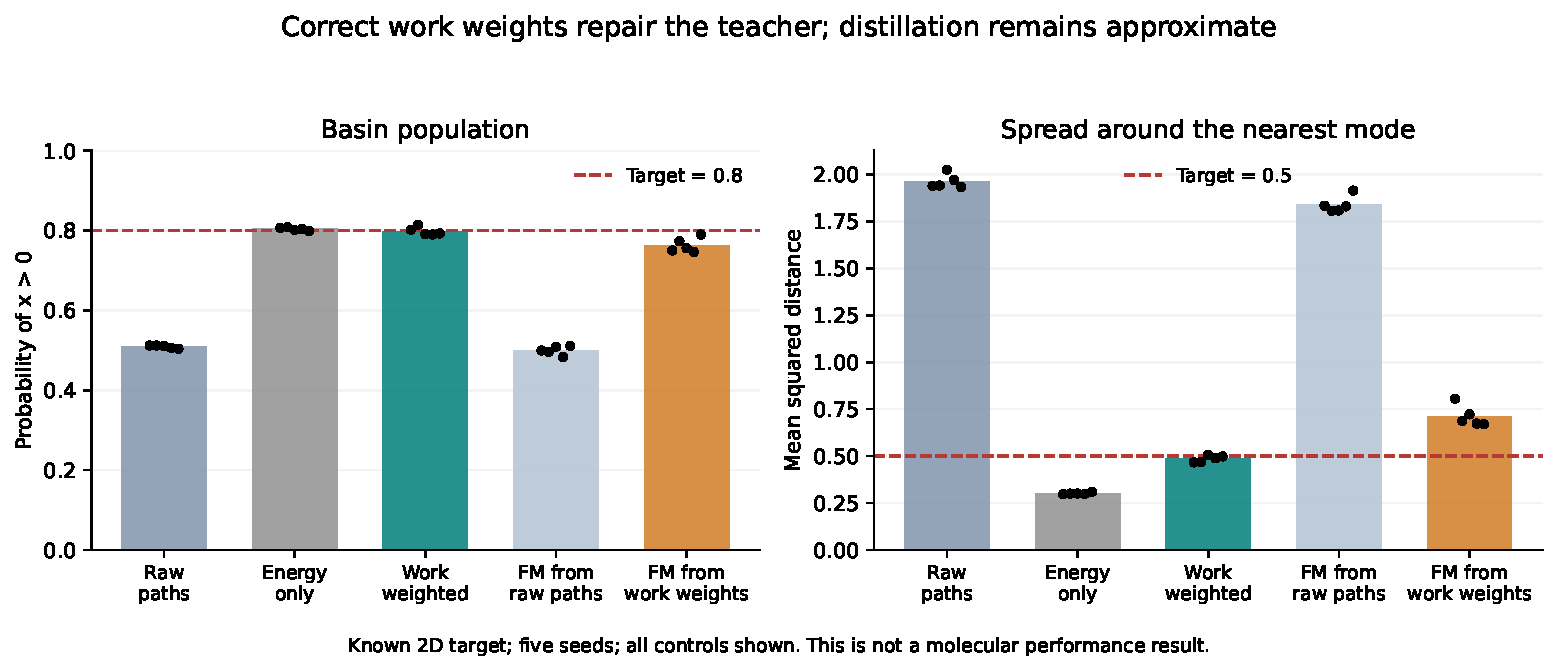
\includegraphics[width=\linewidth]{figures/nonequilibrium_toy.pdf}
\caption{Known-target development control. Bars are means and points show all
five seeds. Red lines are the target statistics. Neither this established
AIS mechanism nor the toy improvement establishes a new molecular method.}
\label{fig:nonequilibriumtoy}
\end{figure}

A first real-model pilot freezes the smoothed displacement FM checkpoint and
uses 32 Gaussian paths with 32 steps, noise scale $0.1$, and auxiliary backward
drift $-v$. The fixed eight-atom validation condition (processed row 5846) has
recorded charge $+1$ and declared singlet multiplicity; original spin metadata
is unavailable. All 32 eSEN evaluations are finite. The declared target is
restrained, $U=E_{\rm eSEN}+0.05\sum_i\|x_i\|^2$ in eV, with $kT=1$ eV.
The resulting ESS is only $1.655/32$ and one endpoint carries $72.87\%$ of the
weight. This establishes executable two-environment inference, while exposing
poor weight efficiency. It is insufficient for a molecular sampling or
generation-advantage claim and does not justify promoting this branch to the
main empirical result.

\paragraph{Raw-source recovery and corrected electronic states.}
Subsequent recovery of the public 4M archive provides 3,986,754 original records.
Replaying preprocessing matches all 3,941,522 accepted records bitwise in the
legacy coordinates, atom types, charge features, forces and rounded energies.
Original charge, spin and float64 energies are retained in separate sidecars.
There are 72,423 charges outside the old feature range and 678,514 non-singlets;
403,895 records have multiplicity above the minimum allowed by electron parity.
An explicit global-state adapter therefore supplies total charge and multiplicity
to the geometry model, replacing the atom-zero total-charge marker.
Matched 10,000-update data-FM continuations, with and without that adapter,
both give 32/32 successful xTB evaluations at the original electronic states.
Median strain is 3.9438 versus 3.8931 eV, respectively.
This is an electronic-state correction, not demonstrated quality improvement.

\paragraph{Independent thermodynamic reference.}
For the neutral AgBr2 doublet (validation row 1137, verified raw row 118392),
rotation-reduced randomized-Sobol integration using analytic Gaussian proposals
gives $\log\widehat Z=144093.1276$ at 3,072 points per scramble and four
independent scrambles. The estimated relative standard error is $1.67\%$,
larger than the final resolution change of 0.00146 nat. It is a statistical
reference rather than exact truth. In three-seed direct importance sampling
with 1,024 potential queries per seed, the confinement Gaussian attains mean
weight ESS 233.85 and mean absolute log-normalizer error 0.05897 nat.
The defensive ordinary and symmetry-averaged template mixtures attain ESS
44.52 and 90.35, with errors 0.15055 and 0.09840 nat. Thus symmetry averaging
helps the template proposal in this experiment but does not surpass the simple
Gaussian reference proposal. The harder eight-atom system remains strongly
weight-degenerate. Neither corrected theory nor these implementation checks
establish improved molecular generation or converged sampling on the broader
system panel.


\end{document}
